% Options for packages loaded elsewhere
\PassOptionsToPackage{unicode}{hyperref}
\PassOptionsToPackage{hyphens}{url}
\PassOptionsToPackage{dvipsnames,svgnames,x11names}{xcolor}
%
\documentclass[
  letterpaper,
  twoside,
  twocolumn,
  9pt]{article}

\usepackage{amsmath,amssymb}
\usepackage{iftex}
\ifPDFTeX
  \usepackage[T1]{fontenc}
  \usepackage[utf8]{inputenc}
  \usepackage{textcomp} % provide euro and other symbols
\else % if luatex or xetex
  \usepackage{unicode-math}
  \defaultfontfeatures{Scale=MatchLowercase}
  \defaultfontfeatures[\rmfamily]{Ligatures=TeX,Scale=1}
\fi
\usepackage{lmodern}
\ifPDFTeX\else  
    % xetex/luatex font selection
\fi
% Use upquote if available, for straight quotes in verbatim environments
\IfFileExists{upquote.sty}{\usepackage{upquote}}{}
\IfFileExists{microtype.sty}{% use microtype if available
  \usepackage[]{microtype}
  \UseMicrotypeSet[protrusion]{basicmath} % disable protrusion for tt fonts
}{}
\usepackage{xcolor}
\usepackage[left=1.5cm,right=1.5cm,top=1.785cm,bottom=2.0cm]{geometry}
\setlength{\emergencystretch}{3em} % prevent overfull lines
\setcounter{secnumdepth}{5}
% Make \paragraph and \subparagraph free-standing
\makeatletter
\ifx\paragraph\undefined\else
  \let\oldparagraph\paragraph
  \renewcommand{\paragraph}{
    \@ifstar
      \xxxParagraphStar
      \xxxParagraphNoStar
  }
  \newcommand{\xxxParagraphStar}[1]{\oldparagraph*{#1}\mbox{}}
  \newcommand{\xxxParagraphNoStar}[1]{\oldparagraph{#1}\mbox{}}
\fi
\ifx\subparagraph\undefined\else
  \let\oldsubparagraph\subparagraph
  \renewcommand{\subparagraph}{
    \@ifstar
      \xxxSubParagraphStar
      \xxxSubParagraphNoStar
  }
  \newcommand{\xxxSubParagraphStar}[1]{\oldsubparagraph*{#1}\mbox{}}
  \newcommand{\xxxSubParagraphNoStar}[1]{\oldsubparagraph{#1}\mbox{}}
\fi
\makeatother


\providecommand{\tightlist}{%
  \setlength{\itemsep}{0pt}\setlength{\parskip}{0pt}}\usepackage{longtable,booktabs,array}
\usepackage{calc} % for calculating minipage widths
% Correct order of tables after \paragraph or \subparagraph
\usepackage{etoolbox}
\makeatletter
\patchcmd\longtable{\par}{\if@noskipsec\mbox{}\fi\par}{}{}
\makeatother
% Allow footnotes in longtable head/foot
\IfFileExists{footnotehyper.sty}{\usepackage{footnotehyper}}{\usepackage{footnote}}
\makesavenoteenv{longtable}
\usepackage{graphicx}
\makeatletter
\newsavebox\pandoc@box
\newcommand*\pandocbounded[1]{% scales image to fit in text height/width
  \sbox\pandoc@box{#1}%
  \Gscale@div\@tempa{\textheight}{\dimexpr\ht\pandoc@box+\dp\pandoc@box\relax}%
  \Gscale@div\@tempb{\linewidth}{\wd\pandoc@box}%
  \ifdim\@tempb\p@<\@tempa\p@\let\@tempa\@tempb\fi% select the smaller of both
  \ifdim\@tempa\p@<\p@\scalebox{\@tempa}{\usebox\pandoc@box}%
  \else\usebox{\pandoc@box}%
  \fi%
}
% Set default figure placement to htbp
\def\fps@figure{htbp}
\makeatother

%%% Preamble of the RSC article template (2016), adapted for Quarto/Pandoc.
%%% Packages Quarto already loads (graphicx, hyperref, natbib, geometry) are omitted; epstopdf is not needed.
\usepackage{extsizes}
% extsizes resets the page layout; Quarto loads geometry first, so the RSC margins are applied again here
\geometry{left=1.5cm,right=1.5cm,top=1.785cm,bottom=2.0cm}
\usepackage[version=3]{mhchem}
\usepackage{balance}
\usepackage{mathptmx}
\usepackage{sectsty}
\usepackage{lastpage}
\usepackage[format=plain,justification=justified,singlelinecheck=false,font={stretch=1.125,small,sf},labelfont=bf,labelsep=space]{caption}
\usepackage{float}
\usepackage{fancyhdr}
\usepackage{fnpos}
\usepackage[english]{babel}
\addto{\captionsenglish}{%
  \renewcommand{\refname}{Notes and references}
}
\usepackage{array}
\usepackage{droidsans}
\usepackage{charter}
\usepackage[T1]{fontenc}
\usepackage[usenames,dvipsnames]{xcolor}
\usepackage{setspace}
\usepackage[compact]{titlesec}
\usepackage{placeins}
\definecolor{cream}{RGB}{222,217,201}

%%% Unicode characters in the text that pdfLaTeX does not map by default
\DeclareUnicodeCharacter{2212}{\ensuremath{-}}
\DeclareUnicodeCharacter{2265}{\ensuremath{\geq}}
\DeclareUnicodeCharacter{03C1}{\ensuremath{\rho}}

%%% Journal artwork for the header and footer, shipped with this extension
\usepackage{booktabs}
\usepackage{longtable}
\usepackage{array}
\usepackage{multirow}
\usepackage{wrapfig}
\usepackage{float}
\usepackage{colortbl}
\usepackage{pdflscape}
\usepackage{tabu}
\usepackage{threeparttable}
\usepackage{threeparttablex}
\usepackage[normalem]{ulem}
\usepackage{makecell}
\usepackage{xcolor}
\usepackage{caption}
\usepackage{anyfontsize}
\makeatletter
\@ifpackageloaded{caption}{}{\usepackage{caption}}
\AtBeginDocument{%
\ifdefined\contentsname
  \renewcommand*\contentsname{Table of contents}
\else
  \newcommand\contentsname{Table of contents}
\fi
\ifdefined\listfigurename
  \renewcommand*\listfigurename{List of Figures}
\else
  \newcommand\listfigurename{List of Figures}
\fi
\ifdefined\listtablename
  \renewcommand*\listtablename{List of Tables}
\else
  \newcommand\listtablename{List of Tables}
\fi
\ifdefined\figurename
  \renewcommand*\figurename{Figure}
\else
  \newcommand\figurename{Figure}
\fi
\ifdefined\tablename
  \renewcommand*\tablename{Table}
\else
  \newcommand\tablename{Table}
\fi
}
\@ifpackageloaded{float}{}{\usepackage{float}}
\floatstyle{ruled}
\@ifundefined{c@chapter}{\newfloat{codelisting}{h}{lop}}{\newfloat{codelisting}{h}{lop}[chapter]}
\floatname{codelisting}{Listing}
\newcommand*\listoflistings{\listof{codelisting}{List of Listings}}
\makeatother
\makeatletter
\makeatother
\makeatletter
\@ifpackageloaded{caption}{}{\usepackage{caption}}
\@ifpackageloaded{subcaption}{}{\usepackage{subcaption}}
\makeatother

\usepackage[super,sort,compress,comma]{natbib}
\bibliographystyle{rsc}
\usepackage{bookmark}

\IfFileExists{xurl.sty}{\usepackage{xurl}}{} % add URL line breaks if available
\urlstyle{same} % disable monospaced font for URLs
\hypersetup{
  pdftitle={Coordinating bioenergy, biochar, and geological storage for biomass-based carbon dioxide removal},
  colorlinks=true,
  linkcolor={blue},
  filecolor={Maroon},
  citecolor={Blue},
  urlcolor={Blue},
  pdfcreator={LaTeX via pandoc}}


\title{Coordinating bioenergy, biochar, and geological storage for
biomass-based carbon dioxide removal}
\author{}
\date{}

\begin{document}
%%% Front matter of the RSC article template (2016), replacing Quarto's \maketitle and abstract.
%%% Title and abstract come from the document metadata; authors, affiliation footnotes and the ESI note
%%% from rsc-authors, rsc-affiliations and rsc-esi.

\pagestyle{fancy}
\thispagestyle{plain}
\fancypagestyle{plain}{
\renewcommand{\headrulewidth}{0pt}
}

%%%PAGE SETUP%%%
\makeFNbottom
\makeatletter
\renewcommand\LARGE{\@setfontsize\LARGE{15pt}{17}}
\renewcommand\Large{\@setfontsize\Large{12pt}{14}}
\renewcommand\large{\@setfontsize\large{10pt}{12}}
\renewcommand\footnotesize{\@setfontsize\footnotesize{7pt}{10}}
\makeatother

\renewcommand{\thefootnote}{\fnsymbol{footnote}}
\renewcommand\footnoterule{\vspace*{1pt}%
\color{cream}\hrule width 3.5in height 0.4pt \color{black}\vspace*{5pt}}
\setcounter{secnumdepth}{5}

\makeatletter
\renewcommand\@biblabel[1]{#1}
\renewcommand\@makefntext[1]%
{\noindent\makebox[0pt][r]{\@thefnmark\,}#1}
\makeatother
\renewcommand{\figurename}{\small{Fig.}~}
\sectionfont{\sffamily\Large}
\subsectionfont{\normalsize}
\subsubsectionfont{\bf}
\setstretch{1.125}
\setlength{\skip\footins}{0.8cm}
\setlength{\footnotesep}{0.25cm}
\setlength{\jot}{10pt}
\titlespacing*{\section}{0pt}{4pt}{4pt}
\titlespacing*{\subsection}{0pt}{15pt}{1pt}

%%%FOOTER%%%
% Page range in the footer: the article ends at the label ArticleLastPage, set before the ESI; the ESI block
% redefines \rscpagerange as S1--\pageref{LastPage}
\providecommand{\rscpagerange}{1--\pageref*{ArticleLastPage}}
\fancyfoot{}
% The template's footer artwork (LF: journal copyright line; RF: "Journal Name, [year], [vol.]") is omitted
% at submission; only the page range and page number are shown
\fancyfoot[RO]{\footnotesize{\sffamily{\rscpagerange ~\textbar  \hspace{2pt}\thepage}}}
\fancyfoot[LE]{\footnotesize{\sffamily{\thepage~\textbar\hspace{2pt} \rscpagerange}}}
\fancyhead{}
\renewcommand{\headrulewidth}{0pt}
\renewcommand{\footrulewidth}{0pt}
\setlength{\arrayrulewidth}{1pt}
\setlength{\columnsep}{6.5mm}
\setlength\bibsep{1pt}

%%%FIGURE SETUP%%%
\makeatletter
\newlength{\figrulesep}
\setlength{\figrulesep}{0.5\textfloatsep}
\newcommand{\topfigrule}{\vspace*{-1pt}%
\noindent{\color{cream}\rule[-\figrulesep]{\columnwidth}{1.5pt}} }
\newcommand{\botfigrule}{\vspace*{-2pt}%
\noindent{\color{cream}\rule[\figrulesep]{\columnwidth}{1.5pt}} }
\newcommand{\dblfigrule}{\vspace*{-1pt}%
\noindent{\color{cream}\rule[-\figrulesep]{\textwidth}{1.5pt}} }
\makeatother

%%%TITLE, AUTHORS AND ABSTRACT%%%
\twocolumn[
  \begin{@twocolumnfalse}
\noindent{
\includegraphics[height=30pt]{journal_name}\hfill\raisebox{0pt}[0pt][0pt]{
\includegraphics[height=55pt]{RSC_LOGO_CMYK}}\\[1ex]

\includegraphics[width=18.5cm]{header_bar}}\par
\vspace{1em}
\sffamily
\begin{tabular}{m{4.5cm} p{13.3cm} } % 13.5cm in the template, which overruns the text block by 7 pt


\includegraphics{DOI} & \noindent\LARGE{\textbf{Coordinating bioenergy,
biochar, and geological storage for biomass-based carbon dioxide
removal\textsuperscript{\dag}}} \\
\vspace{0.3cm} & \vspace{0.3cm} \\

 & \noindent\large{Dominic Woolf,\(^{\ast}\)\textit{$^{a}$} Jocelyn M.
Lavallee,\textit{$^{b}$} Anna M. Raffeld,\textit{$^{b}$} and Doria R.
Gordon\textit{$^{b,c}$}} \\

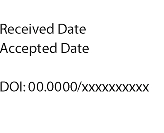
\includegraphics{dates} & \noindent\normalsize{} \\

\end{tabular}

 \end{@twocolumnfalse} \vspace{0.6cm}

  ]

%%%FONT SETUP%%%
\renewcommand*\rmdefault{bch}\normalfont\upshape
\rmfamily
\section*{}
\vspace{-1cm}

%%%FOOTNOTES%%%
\footnotetext{\textit{$^{a}$~College of Agriculture and Life Sciences, Cornell University, Ithaca, NY 14853, USA. E-mail: d.woolf@cornell.edu}}
\footnotetext{\textit{$^{b}$~Environmental Defense Fund, Washington, DC 20090, USA.}}
\footnotetext{\textit{$^{c}$~Department of Biology, University of Florida, Gainesville, FL 32611, USA.}}
\footnotetext{\dag~Electronic supplementary information (ESI)
available.}


\section*{Abstract}\label{abstract}
\addcontentsline{toc}{section}{Abstract}

Crop residues are an abundant biomass source for carbon dioxide removal
(CDR) that requires no additional land. However, the best allocation of
this finite resource among removal technologies is unresolved. We
compared the net costs and benefits of allocating residues to bioenergy,
bioenergy with carbon capture and storage (BECCS), and pyrogenic carbon
capture and storage (PyCCS; biochar applied to soil) at 0.1° spatial
resolution across the United States, Europe, China, and India. PyCCS is
the least-cost removal at moderate carbon prices, mainly through its
agronomic value. In China and India PyCCS abates 110 Tg
CO\textsubscript{2}e yr\textsuperscript{-1}, without requiring a price
on carbon. Across the four regions it abates 650 Tg CO\textsubscript{2}e
yr\textsuperscript{-1} at 100 US\$ Mg\textsuperscript{-1}
CO\textsubscript{2}e. BECCS stores 2.2--2.5 times more carbon per
megagram of residue, and is preferred to PyCCS above regional median
crossover prices of 130--210 US\$ Mg\textsuperscript{-1}
CO\textsubscript{2}e, raising total abatement to 2,030 Tg
CO\textsubscript{2}e yr\textsuperscript{-1} at 250 US\$
Mg\textsuperscript{-1} CO\textsubscript{2}e. These crossover prices
differ between locations, so a universal supply curve would misrepresent
both the carbon price and where each technology is preferred. Bioenergy
without CCS is rarely the best use of residues, once carbon prices are
high enough to make it profitable. Along carbon-price trajectories for
limiting warming to below 2 °C, BECCS can outcompete PyCCS within the
operating life of the PyCCS plant, in which case building BECCS directly
would provide more abatement. Climate strategies should plan for
sequential deployment of PyCCS and BECCS to maximize abatement, while
avoiding lock-in to transitional technologies.

\section*{Broader context}\label{broader-context}
\addcontentsline{toc}{section}{Broader context}

Limiting global warming to below 2 °C requires gigatonne-scale carbon
dioxide removal (CDR), yet expanding dedicated bioenergy crops risks
competing for land with food production and natural ecosystems.
Sustainably harvestable crop residues avoid this land competition, but
the supply of residue is finite. Climate policy therefore faces an
unresolved allocation challenge: should agricultural residues be left in
field, burned to displace fossil power (BE), combusted with geological
carbon capture and storage (BECCS), or pyrolyzed into biochar for soil
application (PyCCS)? Global integrated assessment models rely heavily on
BECCS and rarely represent biochar, whereas facility-level life-cycle
assessments evaluate individual technologies without forcing them to
compete for the same feedstock. By resolving this competition at 0.1°
resolution across the United States, Europe, China, and India, we show
that PyCCS and BECCS are complements ordered by carbon price rather than
mutually exclusive alternatives. PyCCS provides the most cost-effective
early removal, paid for in part by higher crop yields on less fertile
soils, whereas BECCS maximizes total carbon removal from finite biomass
once carbon prices rise and shared CO\textsubscript{2} pipeline networks
are built. Coordinating where and when each technology is deployed can
accelerate near-term CDR while avoiding multi-gigatonne lock-in to
lower-abatement pathways.

\section{Introduction}\label{introduction}

Limiting global warming to below 2 °C requires carbon dioxide removal
(CDR) to counterbalance residual greenhouse gas (GHG) emissions and
reach net-negative emissions later in the
century.\citep{unfccc2015paris, ipcc2022wg3} Biomass can supply CDR, but
dedicated bioenergy crops compete directly with food production and
natural ecosystems for arable land.\citep{fuss2018} Crop residues avoid
this competition: sustainably harvestable residues, after retaining
sufficient biomass to prevent soil erosion and accounting for use as
livestock feed, offer an abundant, spatially dispersed carbon
feedstock.\citep{karan2023, della2026productivity} Because this residue
resource is finite, allocating it across competing climate mitigation
technologies is a critical optimization
challenge.\citep{yue2025managing}

Three thermochemical conversion technologies can compete for available
agricultural residues. Bioenergy (BE) combusts residues to generate
electricity, abating emissions only by displacing fossil power
generation before its biogenic carbon returns to the atmosphere.
Bioenergy with carbon capture and storage (BECCS) captures this
combustion CO\textsubscript{2} and injects it into deep geological
formations, isolating roughly 90\% of feedstock carbon from the
atmosphere.\citep{fuss2018} Pyrogenic carbon capture and storage (PyCCS)
pyrolyzes biomass into biochar for soil (or other) application,
stabilizing 35--42\% of the carbon for centuries while exporting surplus
energy.\citep{schmidt2019pyccs, woolf2010, lehmann2021biochar} Each
approach presents distinct trade-offs. BE requires no
CO\textsubscript{2} disposal infrastructure, but its GHG abatement
diminishes as electricity grids decarbonize. BECCS achieves roughly
double the net CDR per megagram of biomass compared to
PyCCS,\citep{woolf2016optimal} yet it is more capital-intensive and
requires CO\textsubscript{2} pipeline networks and geological sinks.
PyCCS avoids CO\textsubscript{2} transport networks and can raise crop
yields, neutralize soil acidity, and improve nutrient use
efficiency,\citep{jeffery2017, xu2021, yang2025biochar} but it
sequesters less carbon per unit of feedstock. Which technology delivers
the greatest net benefit depends on local soil properties, crop values,
power prices, grid emission intensities, and proximity to geological
storage.\citep{woolf2016optimal}

Current climate policy scenarios do not resolve this geographic and
economic competition. Integrated assessment models (IAMs) rely
predominantly on BECCS for engineered CDR and rarely represent biochar
systems.\citep{ipcc2022wg3, edwards2026state} Operating across coarse
geopolitical regions, IAMs cannot represent the fine-scale heterogeneity
in soils, energy grids, and transport logistics that governs technology
performance. Conversely, bottom-up life-cycle assessments typically
evaluate single technologies in isolation \citep{roe2021} or examine
localized facility case studies.\citep{peters2015, lefebvre2021} By
assessing technologies independently without forcing them to compete for
the same feedstock base, existing studies cannot determine where or at
what carbon price one technology outcompetes
another.\citep{saldarriaga2025biochar} Here, we reconcile
single-facility assessments and global economic models through a
bottom-up, spatially explicit comparison of BE, BECCS, and PyCCS. We
compared the three technologies using MERIDIAN version 1.0, a spatially
explicit model of the costs, revenues, and GHG abatement of biomass use
for energy and CDR (see Methods).

\section{Modeling approach}\label{modeling-approach}

We analyze sustainably available crop residues across the coterminous
United States, Europe, Mainland China, and India at 0.1° resolution.
These four regions capture diverse agricultural soils, energy market
structures, and geological storage capacity, facilitating a granular
modeling approach based on more detailed geographic and economic
analysis than is generally possible at global scales, while illustrating
how diverse local and regional conditions combine to determine optimal
biomass use. At each grid cell, we evaluate the costs, revenues, and GHG
abatement of each technology across a broad range of carbon prices,
allocating residue to the technology with the highest discounted net
value, in which GHG abatement is valued at the carbon price. The
optimization incorporates capital, operating, and maintenance costs;
localized residue collection logistics; crop yield and soil
N\textsubscript{2}O responses to biochar; cost-minimized
CO\textsubscript{2} pipeline routes to characterized geological basins;
price-dependent electricity grid decarbonization; and GHG abatement.
Non-CO\textsubscript{2} GHGs are converted to CO\textsubscript{2}
equivalents using IPCC AR6 100-year global warming
potentials.\citep{forster2021} This analysis establishes the least-cost
spatial allocation of crop residues, identifies the environmental and
infrastructural conditions that set the crossover prices between
technologies, and quantifies the parametric uncertainties that determine
deployment strategy.

The available residue at each grid cell is the sustainably harvestable
residue minus the share fed to livestock (Methods: Crop residue supply).
This residue supplies a conversion facility of specified size, which
draws its feedstock from a circular catchment around the cell. The
catchment is larger where residue is sparse, and haulage cost and
emissions grow with the travel time and road distance from field to
conversion facility (Methods: Biomass transport costs and emissions).

The technologies differ in what they do with the residue carbon
(Methods: Conversion technologies and thermodynamics). BE combusts the
residue and exports electricity. BECCS adds post-combustion
CO\textsubscript{2} capture and sends the CO\textsubscript{2} to
geological storage. For each cell, the CO\textsubscript{2} is assumed to
go to the storage basin with the lowest combined cost of transport and
storage, by pipeline, ship, or sub-sea pipeline (Methods: Carbon
transport and geological storage). Over long distances, plants share
trunklines. PyCCS pyrolyzes the residue to biochar, which is applied to
the cropland of the same cell. Combustion of pyrolysis volatiles and
gases supplies the process heat, and the surplus is either exported as
electricity or heat, or flared. The biochar carbon credited as stored is
the fraction expected to remain after 100 years, which depends on soil
temperature and the biochar's hydrogen-to-carbon ratio (Methods: Biochar
carbon storage). The bottom ash of BE and BECCS is assumed to be
returned to cropland for its plant-nutrient content.

Net GHG abatement is calculated per unit mass of residue, relative to
leaving the residue in the field (Methods: Net GHG abatement). It is the
sum of the CDR and avoided emissions, minus any new emissions. CDR and
avoided emissions include the carbon stored, the grid emissions
displaced by exported electricity, the soil N\textsubscript{2}O
emissions avoided by biochar, and the open-burning emissions avoided
where residue would otherwise be burned in the field. New emissions
include those from haulage, field operations, and CO\textsubscript{2}
transport. Soil GHG emissions resulting from residue removal are not
included, because the net effect of residue removal is approximately
GHG-neutral: the loss of soil organic carbon is offset by lower
N\textsubscript{2}O emissions \citep{mcclelland2025} (Methods: Residue
removal counterfactual). The emission intensity of the displaced
electricity declines as the carbon price rises, following a curve
calibrated to integrated assessment scenarios (see Grid displacement). A
high carbon price is therefore never combined with a fossil-dominated
grid, and the abatement credited to exported electricity falls as the
carbon price rises.

The net value of a technology in a grid cell is its revenue minus its
costs (Methods: Economic evaluation and technology selection). Revenue
comes from electricity sales, net GHG abatement valued at the carbon
price, and the agronomic value of biochar or ash. Costs are capital;
operation and maintenance; feedstock; haulage; and, for BECCS,
CO\textsubscript{2} transport and storage. All three technologies also
pay for the nutrients and alkalinity removed from the field with the
residue. The agronomic value of biochar is the cost of the agricultural
lime (pH amendment) and fertilizer it displaces, plus the value of any
crop yield increase from raising the cation exchange capacity (CEC) of
the soil. The yield response was estimated by meta-regression of field
trials (Methods: Biochar agronomic valuation). All values are levelized
annual values per unit mass of residue, discounted at regional market
costs of capital (discount rates). Results at a social discount rate of
2\% are also reported in the SI.

In each grid cell and at each carbon price, residue is allocated to the
technology with the highest discounted net value, provided that value is
non-negative. Three quantities summarize the results. The
\emph{break-even carbon price} of a technology is the lowest carbon
price at which its net value is non-negative. The \emph{upper-range
technology} of a grid cell is the technology to which it is allocated at
the highest carbon price evaluated, and the \emph{crossover price} is
the lowest carbon price above which the cell remains allocated to that
technology. The abatement supply curve of a region is the net GHG
abatement of all allocated cells, summed over the region, as a function
of the carbon price.

Two analyses identify the drivers of these quantities. A Monte Carlo
analysis propagates parameter uncertainty to the regional break-even and
crossover prices (Methods: Monte Carlo analysis). Regression models of
the grid-cell results attribute the spatial variation of these prices to
spatial inputs, such as soil properties, crop value, electricity price,
and distance to CO\textsubscript{2} storage (Methods: Spatial drivers of
cost). Both use SHAP (SHapley Additive exPlanations) values to attribute
each result to its inputs. Plant size, the sharing of
CO\textsubscript{2} pipelines, and the use of
CO\textsubscript{2}-enhanced oil recovery sites as sinks are design
choices rather than uncertain or spatially-varying parameters , and
their effects are reported as variants (Methods: Structural variants).

\section{Results}\label{results}

Each technology was evaluated at carbon prices from 0 to 500 US\$
Mg\textsuperscript{-1} CO\textsubscript{2}e. Where a single price is
quoted, we use 100 US\$ Mg\textsuperscript{-1} CO\textsubscript{2}e,
close to the marginal abatement cost of CO\textsubscript{2} in 2030 (119
US\$ Mg\textsuperscript{-1}) in mitigation pathways likely to limit
warming to below 2 °C;\citep{riahi2022} results across the full range
are shown in Figure~\ref{fig-macc} and Figure~\ref{fig-break-even}.

\begin{figure}

\centering{

\includegraphics[width=1\linewidth,height=\textheight,keepaspectratio]{MACC.png}

}

\caption{\label{fig-macc}Abatement supply curves: annual abatement of
the technology with the highest non-negative net value in each grid
cell, summed over each region, as a function of the carbon price, at the
regional market discount rates.}

\end{figure}%

\begin{figure*}[t]

\centering{

\includegraphics[width=1\linewidth,height=\textheight,keepaspectratio]{Breakeven_CPrice.png}

}

\caption{\label{fig-break-even}Break-even carbon price of each
technology (rows 1--3), the technology with the lowest break-even price
(row 4) and that price (row 5), by region (columns), at the regional
market discount rates. The break-even price is the carbon price at which
the net value of a technology becomes non-negative; it is negative where
a technology is profitable without a carbon price. The technology with
the lowest break-even price is the first to become profitable as the
carbon price rises, but not necessarily the one with the highest net
value at higher prices (Figure~\ref{fig-evap}). Colors are capped at −50
and 200 US\$ Mg\textsuperscript{-1} CO\textsubscript{2}e.}

\end{figure*}%

\subsection{Abatement potential rises in two steps as the carbon price
increases}\label{abatement-potential-rises-in-two-steps-as-the-carbon-price-increases}

Summing the abatement of the technology with the highest non-negative
net value in each grid cell gives an abatement supply curve for each
region (Figure~\ref{fig-macc}). Across the four regions, residues abate
119 Tg CO\textsubscript{2}e yr\textsuperscript{-1} without a carbon
price, almost all of it through PyCCS in China and India. Abatement
rises to 543 Tg CO\textsubscript{2}e yr\textsuperscript{-1} at 50 US\$
Mg\textsuperscript{-1} CO\textsubscript{2}e and 709 Tg
CO\textsubscript{2}e yr\textsuperscript{-1} at 100 US\$
Mg\textsuperscript{-1} CO\textsubscript{2}e, 92\% of it from PyCCS. It
then rises more steeply as BECCS becomes viable, to 1,386 Tg
CO\textsubscript{2}e yr\textsuperscript{-1} at 150 US\$
Mg\textsuperscript{-1} CO\textsubscript{2}e and 1,888 Tg
CO\textsubscript{2}e yr\textsuperscript{-1} at 200 US\$
Mg\textsuperscript{-1} CO\textsubscript{2}e, and reaches 2,034 Tg
CO\textsubscript{2}e yr\textsuperscript{-1} at 250 US\$
Mg\textsuperscript{-1} CO\textsubscript{2}e, 99\% of it from BECCS. In
the first step, abatement grows as PyCCS becomes profitable on more
residue. In the second, the same residue is reallocated to the
technology that stores more carbon per megagram. In China and India, all
residue is already in use at 100 US\$ Mg\textsuperscript{-1}
CO\textsubscript{2}e (Figure~\ref{fig-si-macc-biomass}), so all further
abatement comes from reallocation: abatement in China nearly doubles,
from 418 Tg CO\textsubscript{2}e yr\textsuperscript{-1} at 100 US\$
Mg\textsuperscript{-1} CO\textsubscript{2}e to 798 Tg
CO\textsubscript{2}e yr\textsuperscript{-1} at 200 US\$
Mg\textsuperscript{-1} CO\textsubscript{2}e. In the United States, both
steps occur at higher prices: PyCCS between 100 and 150 US\$
Mg\textsuperscript{-1} CO\textsubscript{2}e, and BECCS between 150 and
250 US\$ Mg\textsuperscript{-1} CO\textsubscript{2}e.

\subsection{Carbon storage outcompetes conventional
bioenergy}\label{carbon-storage-outcompetes-conventional-bioenergy}

Bioenergy without carbon capture (BE) is rarely the optimal use of crop
residues. Without a carbon price, BE loses money across the four
regions: its biomass-weighted mean net value is negative in all Monte
Carlo draws for the United States and China, and positive in at most
1.4\% of draws for Europe and India. However, lowering the discount rate
to a 2\% social discount rate (a rate reflecting society's valuation of
future costs and benefits) makes BE cost-effective without a carbon
price on 43\% of the residue in Europe (Figure S2). Even with a carbon
price, its climate benefit remains small. Because the electricity
displaced by BE becomes cleaner as power grids decarbonize, its
mitigation value drops as carbon prices rise. At 100 US\$
Mg\textsuperscript{-1} CO\textsubscript{2}e, BE abates only 0.14--0.24
Mg CO\textsubscript{2}e per megagram of residue. This specific abatement
is only 17--30\% of the GHG abatement achieved by pyrogenic carbon
capture and storage (PyCCS), and less than 14\% of that achieved by
bioenergy with carbon capture and storage (BECCS). Consequently, BE is
the leading use of residues only where displaced electricity remains
carbon-intensive, mainly in Europe at low carbon prices where BE
captures 26\% of the European residue at 50 US\$ Mg\textsuperscript{-1}
CO\textsubscript{2}e, primarily in Ukraine, Moldova, and southeastern
Europe (Figure~\ref{fig-evap}). Any increase in carbon price favors
technologies that physically store carbon over those that merely
displace fossil electricity, because electricity grids decarbonize at
higher carbon prices, which reduces the emissions that BE can displace.
Because of this covariance between carbon prices and grid intensity, the
GHG abatement of BE per megagram of residue falls by 68--83\% between
carbon prices of 0 and 200 US\$ Mg\textsuperscript{-1}
CO\textsubscript{2}e, compared with 7--23\% for BECCS and at most 36\%
for PyCCS, which also export electricity but derive most of their
abatement from stored carbon.

\begin{figure*}[t]

\centering{

\includegraphics[width=1\linewidth,height=\textheight,keepaspectratio]{Evaporation_Grid_market.png}

}

\caption{\label{fig-evap}Technology with the highest net value in each
grid cell, by carbon price (rows) and region (columns), at the regional
market discount rates. Saturated colors indicate that net value is
positive; pale colors indicate that no technology is profitable, and the
color shows the one with the smallest loss.}

\end{figure*}%

\subsection{Biochar delivers the most cost-effective early CDR driven by
agronomic
co-benefits}\label{biochar-delivers-the-most-cost-effective-early-cdr-driven-by-agronomic-co-benefits}

The four regions provide 1,252 Tg yr\textsuperscript{-1} of available
crop residue on a dry, ash-free basis (Methods: Crop residue supply). At
a carbon price of 100 US\$ Mg\textsuperscript{-1} CO\textsubscript{2}e,
PyCCS is the technology with the highest non-negative net value for 99\%
of this residue in China, 85\% in India, and 48\% in Europe
(Figure~\ref{fig-evap}). At this price, PyCCS abates 650 Tg
CO\textsubscript{2}e yr\textsuperscript{-1} across the four regions,
92\% of the total economically viable GHG abatement
(Figure~\ref{fig-macc}). PyCCS breaks even (its net value becomes
positive) at a lower carbon price than BECCS on 79--100\% of the residue
in each region (Figure~\ref{fig-break-even}).

Despite providing half the CDR as BECCS, PyCCS outcompetes geological
storage at moderate prices because biochar generates a direct agronomic
return. At 100 US\$ Mg\textsuperscript{-1} CO\textsubscript{2}e, biochar
applied to cropland provides value equivalent to 64 and 68 US\$
Mg\textsuperscript{-1} of feedstock in China and India. Crop yield
increases contribute 44 and 42 US\$ Mg\textsuperscript{-1} to this
total, respectively, with the replacement of agricultural lime,
phosphorus, and potassium accounting for the remainder. This agronomic
value is lower in the United States and Europe, at 38 and 24 US\$
Mg\textsuperscript{-1} respectively, where yield increases contribute
only 25 and 12 US\$ Mg\textsuperscript{-1} (Methods: Biochar agronomic
valuation and Meta-analysis of biochar field trials). Biochar carbon
sequestration accounts for 78--98\% of the GHG abatement of PyCCS across
the four regions. The grid credit for exported electricity adds 2--18\%.
It is smallest in the United States, where plants processing 93\% of the
residue are predicted to flare their surplus gas rather than generate
electricity (see Results: High feedstock costs and low power prices
delay CDR in the United States). In an exploratory variant where PyCCS
sells all surplus heat rather than electricity to a year-round user
(Methods: Pyrogenic carbon capture and storage), the net value of PyCCS
at 100 US\$ Mg\textsuperscript{-1} CO\textsubscript{2} rises by 21--38
US\$ Mg\textsuperscript{-1} of residue in China, the United States, and
Europe, and by less than 1 US\$ Mg\textsuperscript{-1} in India, while
altering GHG abatement by less than 0.06 Mg CO\textsubscript{2}e
Mg\textsuperscript{-1}. Avoided soil N\textsubscript{2}O emissions add
1--3\% to the PyCCS net abatement.

Because PyCCS economics rely heavily on agricultural returns rather than
energy export, lowering the cost of capital extends its viability to
even lower carbon prices. At a 2\% social discount
rate,\citep{drupp2018} PyCCS is profitable without any carbon price for
50\% of the crop residue in China and 46\% in India
(Figure~\ref{fig-si-evap-social}).

\subsection{High feedstock costs and low power prices delay CDR in the
United
States}\label{high-feedstock-costs-and-low-power-prices-delay-cdr-in-the-united-states}

The United States is an exception among the four regions. Neither CDR
technology (PyCCS or BECCS) is viable at or below 100 US\$
Mg\textsuperscript{-1} CO\textsubscript{2}e on more than 7\% of its
agricultural residue, or 13\% of the land area from which that residue
can be sourced. The share of land area is larger than the share of
residue because the cells where PyCCS is viable have sparser crop
residues. PyCCS becomes the leading use only between 100 and 150 US\$
Mg\textsuperscript{-1} CO\textsubscript{2}e, expanding to cover 93\% of
the residue at the higher price. This delayed viability stems mainly
from feedstock and electricity prices, and partly from a smaller
agronomic return. US feedstock costs are higher than in China and India,
averaging 55 US\$ Mg\textsuperscript{-1} compared to 31--45 US\$
Mg\textsuperscript{-1} in China and India. Simultaneously, low wholesale
electricity prices in the US (Methods: Spatial input data, and Methods:
Capacity factors and price capture of biomass power) depress the
economic value of energy export. Consequently, the power block is
omitted from PyCCS plants for 93\% of the US residue, to avoid capital
losses.

\subsection{Geological storage is preferred at high carbon prices,
maximizing absolute GHG
abatement}\label{geological-storage-is-preferred-at-high-carbon-prices-maximizing-absolute-ghg-abatement}

Above a regional carbon-price threshold, BECCS has a higher net value
than PyCCS and is the leading use of residues. No grid cell allocated to
BECCS at one carbon price is allocated to another technology at a higher
price, and BECCS is the upper-range technology for at least 99.9\% of
the residue in each region. In the remaining cells, BECCS either has no
viable CO\textsubscript{2} route to a storage basin, or would be
preferred only above 500 US\$ Mg\textsuperscript{-1}
CO\textsubscript{2}e. We therefore report the crossover price as the
carbon price above which BECCS is the technology with the highest
non-negative net value. The median crossover price is 132 US\$
Mg\textsuperscript{-1} CO\textsubscript{2}e in India, 154 in China, 176
in Europe, and 207 in the United States. Within each region, the
crossover price differs by 84--121 US\$ Mg\textsuperscript{-1}
CO\textsubscript{2}e between the 10th and 90th percentiles of grid cells
(Figure~\ref{fig-takeover-price}).

\begin{figure*}[t]

\centering{

\includegraphics[width=1\linewidth,height=\textheight,keepaspectratio]{map_takeover_price.png}

}

\caption{\label{fig-takeover-price}Crossover price of BECCS in each grid
cell: the carbon price above which BECCS is the technology with the
highest non-negative net value, at the regional market discount rates.
Gray: BECCS is not preferred at any carbon price up to 500 US\$
Mg\textsuperscript{-1} CO\textsubscript{2}e.}

\end{figure*}%

Because carbon capture recovers roughly 90\% of the feedstock carbon,
BECCS abates 1.69--1.76 Mg CO\textsubscript{2}e per megagram of residue.
This is roughly twice the per-megagram efficiency of PyCCS, which
permanently stores 35--42\% of the initial carbon as biochar.

Allocating residue to BECCS rather than PyCCS at higher carbon prices
therefore maximizes the total GHG abatement obtained from a limited
biomass supply (Figure~\ref{fig-macc}).

\subsection{\texorpdfstring{Soil chemistry and distance to
CO\textsubscript{2} sinks set the crossover
price}{Soil chemistry and distance to CO2 sinks set the crossover price}}\label{soil-chemistry-and-distance-to-co2-sinks-set-the-crossover-price}

The break-even price of PyCCS is governed predominantly by agronomic
conditions, with lower break-even prices where biochar adds most to the
value of the harvest. We attributed the spatial variation in break-even
prices to the model inputs using SHAP (Shapley additive explanation)
values, which divide each grid cell's prediction from a regression model
fitted to the results among the inputs (Methods: Spatial drivers of
cost). Together, crop value per hectare and soil CEC account for 65\% of
the mean absolute SHAP value in China, 76\% in India, and 60\% in the
United States (Figure~\ref{fig-shap-importance}). In contrast, the most
important driver of the break-even price of BECCS is the routed distance
to geological storage, accounting for 42\% in China and 67\% in India.

\begin{figure*}[t]

\centering{

\includegraphics[width=1\linewidth,height=\textheight,keepaspectratio]{shap_importance.png}

}

\caption{\label{fig-shap-importance}Spatial drivers of the carbon prices
at which each technology breaks even or outcompetes another.
(\textbf{a}--\textbf{d}) Share of the mean absolute SHAP value (\%) of
each group of spatial inputs in regional regression models of
(\textbf{a}) the break-even price of PyCCS, (\textbf{b}) the price at
which BECCS outcompetes BE, (\textbf{c}) the break-even price of BECCS,
and (\textbf{d}) the price at which BECCS outcompetes PyCCS, which is
the crossover price of BECCS. The groups are soil and crop (soil
temperature, CEC, and pH; biochar supply per hectare; and crop value per
hectare); residue supply and management (collection distance; the
terrain and road-network multiplier of haulage cost; feedstock cost; and
the share of residue otherwise burned); the electricity grid
(electricity price and displaced grid carbon intensity); and
CO\textsubscript{2} transport and storage (route length, offshore sink,
and storage cost). Shares of individual inputs are given in
Table~\ref{tbl-si-shap-importance}. The value to the right of each bar
is the residue-weighted regional median of that price (US\$
Mg\textsuperscript{-1} CO\textsubscript{2}e). (\textbf{e}) Net value of
each technology per megagram of residue against the carbon price, as the
residue-weighted median over all grid cells of the four regions at each
price. Points a--d mark where these curves cross zero or each other.
Because each curve is a median at each price, not the curve of a single
grid cell, these points can differ from the medians of the prices in
a--d.}

\end{figure*}%

Consequently, the crossover price of BECCS depends on both soils and
CO\textsubscript{2} infrastructure (Figure~\ref{fig-takeover-driver}).
Crop value per hectare is the most common dominant driver of the
crossover price in China and the United States, and soil CEC is the
second most common in India. On productive, low-CEC cropland, biochar
remains the better use up to higher carbon prices. Distance to storage
dominates in most of Europe and in much of India, where the crossover
price is lowest near sinks and highest far from them.

\begin{figure*}[t]

\centering{

\includegraphics[width=1\linewidth,height=\textheight,keepaspectratio]{map_takeover_driver.png}

}

\caption{\label{fig-takeover-driver}Dominant driver of the crossover
price of BECCS (Figure~\ref{fig-takeover-price}) in each grid cell: the
spatial input with the largest absolute SHAP value in the regional
regression model (Figure~\ref{fig-shap-importance}).}

\end{figure*}%

SHAP dependence plots for each input, quantity, and region
(\ref{fig-si-dep-be-pyccs-us}--\ref{fig-si-dep-takeover-beccs-india})
show the form of these effects. In China, the contribution of crop value
to the break-even price of PyCCS declines steadily as crop value rises,
whereas that of soil CEC rises between about 15 and 30
cmol\textsubscript{c} kg\textsuperscript{-1} and changes little above
that range. Break-even prices are also lower where the biochar supply is
below about 1.5 Mg ha\textsuperscript{-1} yr\textsuperscript{-1},
because the yield response per megagram of biochar is largest at low
doses. In India, the contribution of the CO\textsubscript{2} route
length to the crossover price of BECCS rises gradually up to about 750
km and steeply beyond it. The cells more than 800 km from storage,
mostly in northern India, also have soils with a lower CEC, so this step
partly reflects a correlation between inputs that SHAP values do not
separate.

\subsection{\texorpdfstring{BECCS requires shared CO\textsubscript{2}
infrastructure and large
plants}{BECCS requires shared CO2 infrastructure and large plants}}\label{beccs-requires-shared-co2-infrastructure-and-large-plants}

The viability of each technology relies on different prerequisites.
BECCS requires aggregated infrastructure and large-scale deployment to
succeed (Figure~\ref{fig-si-variants}). At 200 US\$
Mg\textsuperscript{-1} CO\textsubscript{2}e, BECCS abates 361 Tg
CO\textsubscript{2}e yr\textsuperscript{-1} in the United States using
125 MW\textsubscript{th} plants, but this falls to 8 Tg
CO\textsubscript{2}e yr\textsuperscript{-1} if restricted to 50
MW\textsubscript{th} plants. Shared CO\textsubscript{2} trunklines
matter as much as plant size. If each facility builds a dedicated
pipeline to a sink, BECCS GHG abatement at 200 US\$
Mg\textsuperscript{-1} CO\textsubscript{2}e falls to 133 Tg
CO\textsubscript{2}e yr\textsuperscript{-1} in the United States, 191 in
Europe, and 502 in China. Under these infrastructure variants (smaller
plants or dedicated pipelines for each BECCS facility), PyCCS becomes
the optimal choice for much of the residue that would otherwise go to
BECCS, because it operates independently of CO\textsubscript{2}
transport networks and scales efficiently at smaller capacities.
Allowing CO\textsubscript{2}-enhanced oil recovery (EOR) sites as sinks
alters regional GHG abatement by less than 5\% at 200 US\$
Mg\textsuperscript{-1} CO\textsubscript{2}e.

\subsection{Parameter uncertainty shifts the crossover prices more than
their
order}\label{parameter-uncertainty-shifts-the-crossover-prices-more-than-their-order}

Uncertainty in the model parameters (Table~\ref{tbl-si-mc}) was
propagated with 5,000 Monte Carlo draws per region (Methods: Monte Carlo
analysis). The order of the break-even prices holds: the regional median
break-even price of PyCCS is below that of BECCS in 93--99\% of draws,
by a median of 38--62 US\$ Mg\textsuperscript{-1} CO\textsubscript{2}e.
The carbon prices at which each technology becomes viable are less
certain. Across the draws, the 90\% ranges of the median crossover price
of BECCS span 84--279 US\$ Mg\textsuperscript{-1} CO\textsubscript{2}e.
Uncertainty in regional abatement is therefore largest at carbon prices
near these thresholds. At 100 US\$ Mg\textsuperscript{-1}
CO\textsubscript{2}e, the 90\% range of abatement in the United States
is 0--219 Tg CO\textsubscript{2}e yr\textsuperscript{-1}, because this
price lies within the 90\% range of the break-even price of PyCCS there
(74--173 US\$ Mg\textsuperscript{-1} CO\textsubscript{2}e). In China,
where the median break-even price of PyCCS is 35 US\$
Mg\textsuperscript{-1} CO\textsubscript{2}e, the range is 391--630 Tg
CO\textsubscript{2}e yr\textsuperscript{-1}.

The crop yield response to biochar dominates the uncertainty in PyCCS
break-even pricing. The parameters defining the yield response account
for 24--26\% of the mean absolute SHAP value in the United States,
China, and India, with assumptions about how rapidly this response
declines over time adding a further 7--10\%. The crossover price of
BECCS inherits both of these sensitivities. It is driven primarily by
agronomic yield uncertainty in China and India, where yield increases
contribute a larger share of the net value of PyCCS, and by capital
costs and capacity factors in the United States and Europe.

\subsection{Building PyCCS early delays the transition to
BECCS}\label{building-pyccs-early-delays-the-transition-to-beccs}

The comparisons above hold the carbon price fixed. A plant, however,
commits its residue for its operating life, during which period carbon
prices may change. Mitigation scenarios typically have carbon prices
that rise over time, for three reasons. First, in scenarios that meet a
temperature goal at least cost, the remaining carbon budget is used like
an exhaustible resource, and the carbon price rises at about the
discount rate.\citep{hotelling1931, emmerling2019} Discounting gives
future mitigation costs less weight than present ones, which defers
abatement to later, deeper, and more expensive cuts. Second, investment
goes first to the least-cost abatement options, so each further cut
requires more expensive options and a higher carbon price. Third, policy
instruments are typically introduced at low carbon prices and raised
gradually, because early policies build the political support and
institutions that greater stringency requires.\citep{pahle2018}

With rising carbon prices, the optimal conversion technology may change
during the operating life of a facility. The more rapidly carbon prices
rise, the more likely it is that BECCS will become optimal during the
lifetime of a PyCCS facility. To quantify the abatement forgone through
\emph{lock-in} (the commitment of residue to a technology by an earlier
investment), we followed cohorts of conversion facilities along the
median marginal abatement cost of CO\textsubscript{2} in mitigation
pathways likely to limit warming to 2 °C.\citep{riahi2022} We use this
trajectory as an illustration rather than a forecast, because the
pathways from which it is drawn largely omit
PyCCS.\citep{edwards2026state} Along this trajectory, our results
predict that 1,030 Tg yr\textsuperscript{-1} of residue is allocated
first to PyCCS and later to BECCS. The median PyCCS plant is built in
2030--2032, and the carbon price reaches the median crossover price of
BECCS (the crossover year) in 2035--2040, within the 20-year life of the
plant.

Once a PyCCS plant is built, its capital is sunk. If its owner switches
to BECCS when the net value of BECCS exceeds that of PyCCS by the
annualized capital cost of the PyCCS plant, the PyCCS operates for 12
years on average, and abatement over 2030--2069 is 5.0 Gt
CO\textsubscript{2}e lower than with a switch in the crossover year.
Running PyCCS plants to the end of their life forgoes 12.5 Gt
CO\textsubscript{2}e. Leaving the residue unused until the crossover
year forgoes as much as the sunk-capital switch, 5.1 Gt
CO\textsubscript{2}e, and has the lowest net present value of all six
strategies.

Building BECCS from the outset on this residue gives the most abatement:
67 Gt CO\textsubscript{2}e over 2030--2069, 10.9 Gt CO\textsubscript{2}e
(19\%) more than PyCCS followed by a sunk-capital switch. Its net
present value, in which abatement is valued at the carbon price of each
year, is 1\% higher across the four regions, ranging from −7\% in the
United States to +6\% in Europe. A capture-ready BE plant that is later
retrofitted with CO\textsubscript{2} capture performs like BECCS built
from the outset, because BECCS has a higher net value than BE in almost
all of these grid cells from the first year (0.2 years of BE operation
on average). These results assume perfect foresight of the carbon price,
no lead time for building BECCS, and CO\textsubscript{2} transport and
storage available from 2030.

Both the advantage of BECCS and the period of lock-in depend on
CO\textsubscript{2} infrastructure and on the rate at which the carbon
price rises. With a dedicated pipeline from each BECCS plant to its sink
instead of shared trunklines, the carbon price reaches the crossover
price of BECCS later, in 2036--2044, and residue stays in PyCCS for 15
years under a sunk-capital switch. Building BECCS from the outset then
gives 13.3 Gt CO\textsubscript{2}e more abatement than PyCCS followed by
a sunk-capital switch, but its net present value is 10\% lower across
the four regions, and lower in every region (−4\% to −29\%). Along a
slower trajectory, that of the NGFS scenario in which countries meet
their nationally determined contributions (75 US\$
Mg\textsuperscript{-1} CO\textsubscript{2}e in 2030, rising to 98 US\$
Mg\textsuperscript{-1} CO\textsubscript{2}e in 2050),\citep{ngfs2026}
PyCCS is built on 811 Tg yr\textsuperscript{-1} of residue. BECCS
outcompetes it before 2069 on only 27 Tg yr\textsuperscript{-1} of this
residue with shared trunklines, and on 7 Tg yr\textsuperscript{-1} with
dedicated pipelines.

\FloatBarrier

\section{Discussion}\label{discussion}

\subsection{Integrating spatial competition into global mitigation
pathways}\label{integrating-spatial-competition-into-global-mitigation-pathways}

Mitigation pathways that limit warming in line with the Paris Agreement
\citep{unfccc2015paris} rely on CDR to offset residual emissions and
reach net-negative emissions later in the century. In the pathways
assessed by the IPCC that are likely to limit warming to 2 °C, BECCS
supplies most of this removal,\citep{ipcc2022wg3, edwards2026state}
sequestering 170--650 Gt CO\textsubscript{2} between 2020 and
2100,\citep{ipcc2022wg3} with a median of about 2.75 Gt
CO\textsubscript{2} yr\textsuperscript{-1} in 2050.\citep{babiker2022}
Biochar (PyCCS) is largely absent from the integrated assessment models
(IAMs) that generate these pathways.\citep{edwards2026state} In our
analysis, however, when forced to compete for the same crop residues
across the United States, Europe, China, and India, PyCCS is the
least-cost CDR technology over a wide range of moderate carbon prices,
whereas BECCS dominates at high carbon prices because it stores more
than twice as much carbon per megagram of residue. The two technologies
are therefore ordered by carbon price rather than interchangeable. Our
results imply that scenarios that omit PyCCS overstate the carbon price
needed to initiate biomass CDR and understate the abatement available
below 150 US\$ Mg\textsuperscript{-1} CO\textsubscript{2}e. Conversely,
adding a low-cost removal option like PyCCS to IAMs would be expected to
lower the near-term marginal abatement cost required to meet a given
carbon budget, which would in turn delay when the crossover price to
BECCS is reached. Even restricted to sustainably available crop residues
in these four regions, our projected maximum abatement at high carbon
prices () reaches three-quarters of the global 2050 BECCS benchmark in 2
°C IPCC pathways.\citep{babiker2022}

Existing IAMs divide the world into a few dozen geopolitical regions and
represent biomass supply and CO\textsubscript{2} transport by aggregate
supply curves or fixed per-megagram charges rather than by the precise
locations of feedstocks and sinks.\citep{gambhir2019} Resolving
technology competition on a 0.1° grid alters these dynamics in three
ways: technology selection responds to local soil properties, crop
values, and grid emission intensities; CO\textsubscript{2} transport
costs reflect terrain-routed pipelines from each plant to characterized
storage basins; and biochar is valued through its local effects on
agriculture. Because feedstock costs, wholesale electricity prices, and
agronomic returns differ sharply across and within regions, delaying
PyCCS adoption in the United States while driving zero-price deployment
in parts of China and India, a universal global supply curve
misrepresents both the carbon price at which each technology is
preferred and where it should be built. Capturing the sequential
transition from PyCCS to BECCS in IAMs requires representing spatial
heterogeneity in crop production, agricultural markets, power prices,
and CO\textsubscript{2} sink access.

\subsection{Agronomic co-benefits, financing levers, and biophysical
uncertainties}\label{agronomic-co-benefits-financing-levers-and-biophysical-uncertainties}

PyCCS is competitive at moderate carbon prices because returning biochar
to the cropland from which residue was harvested generates a revenue
stream independent of the carbon market. Because crop value per hectare
and soil CEC govern most of the spatial variation in PyCCS break-even
prices, early CDR is tightly coupled to agricultural productivity and
food security: PyCCS is most competitive where soils are nutrient-poor
and biochar adds the most value to the harvest. Because PyCCS economics
rely on these multi-decade agricultural returns and upfront capital
rather than electricity sales, the cost of capital is an effective
policy lever for early deployment. Concessional finance, public
investment, or agricultural credit programs that bring project discount
rates toward a 2\% social discount rate could unlock substantial residue
CDR in China and India before carbon markets mature. However, low-cost
capital must be paired with carbon pricing or technology standards: in
Europe, a 2\% discount rate without a carbon price makes unabated BE
profitable across nearly half of the residue supply
(Figure~\ref{fig-si-evap-social}), directing biomass to its
lowest-abatement use.

Dependence on agronomic revenue is also the primary vulnerability of
PyCCS. The parameters governing the crop yield response to biochar are
the largest source of uncertainty in our PyCCS break-even prices. This
uncertainty stems from a mismatch in timescales: the economics of PyCCS
depend on yield and soil N\textsubscript{2}O responses over decades,
whereas most field trials last only one or two years.\citep{kaur2023}
While syntheses of single biochar applications show that
N\textsubscript{2}O reductions and yield benefits diminish as biochar
ages,\citep{borchard2019, kaur2023, yang2025biochar} multi-year
experiments spanning 4--12 years indicate that repeated applications
sustain or increase both benefits.\citep{yang2025biochar} In our
optimization, biochar is reapplied to rotating field cohorts at
intervals of 3--4 years in the United States, China, and India (and 15
years in Europe) at median doses of 5--11 Mg ha\textsuperscript{-1}.
Further long-term field trials with repeat application cycles would help
to constrain this important uncertainty.

\subsection{Navigating temporal lock-in and infrastructure
dependencies}\label{navigating-temporal-lock-in-and-infrastructure-dependencies}

As carbon prices rise over time, the ordering of technologies by price
becomes a sequence in time, creating a trade-off between near-term
deployment and long-term abatement. In our lock-in analysis along a 2 °C
carbon-price trajectory, PyCCS built in the early 2030s commits
feedstock that would achieve roughly double the CDR per megagram if
allocated to BECCS later in the same decade. Building BECCS from the
outset avoids this 5--12 Gt CO\textsubscript{2}e lock-in penalty and
achieves a comparable net present value, but that advantage rests on two
conditions: that carbon prices rise rapidly and that shared
CO\textsubscript{2} trunklines and storage basins are operational from
2030. In 1.5 °C pathways with no or limited overshoot,\citep{riahi2022}
marginal abatement costs exceed our regional crossover prices before
2030. Although \textless1.5 °C without overshoot is no longer widely
believed to be
achievable,\citep{lenton2025global, matthews2022current, tavoni2026implications}
these scenarios demonstrate that ambitious mitigation can justify direct
BECCS investment from the outset where CO\textsubscript{2} storage is
accessible.

In practice, neither rapid carbon price escalation nor immediate
pipeline access is assured. Early CCS networks are expected to establish
around large or high-purity CO\textsubscript{2} point sources such as
fossil fuel power stations, ethanol fermentation, cement production,
ammonia production, and natural gas
processing.\citep{bains2017, sanchez2018} Because crop-residue BECCS
facilities are smaller and more spatially dispersed, their economic
viability depends on joining shared trunklines built for industrial hubs
rather than financing dedicated long-distance pipelines
(Figure~\ref{fig-si-variants}). Where facilities must build dedicated
pipelines, or where realized carbon prices follow the slower trajectory
\citep{ngfs2026} of current nationally determined contributions,
building BECCS directly reduces net present value in our analysis across
all regions and PyCCS remains the superior economic choice for decades.
Because its agronomic revenue is insulated from carbon-market
volatility, PyCCS is a low-regret first step where carbon prices or
CO\textsubscript{2} infrastructure are uncertain. Regional planners can
minimize lock-in during this transition by siting early pyrolysis plants
where crossover prices are highest on productive, low-CEC croplands far
from geological sinks Figure~\ref{fig-takeover-price} while reserving
areas of more fertile soils near emerging CO\textsubscript{2} trunklines
for BECCS.

\subsection{Alternative pathways and technical
boundaries}\label{alternative-pathways-and-technical-boundaries}

Unabated bioenergy (BE) is rarely an effective use of crop residues. As
power grids decarbonize at higher carbon prices, the emissions displaced
by exported electricity fall sharply. Although co-firing residues in
existing coal plants may lower capital costs and directly displace
coal,\citep{roni2017} its mitigation value is bounded by the remaining
operating life of coal fleets and by boiler limits on high-alkali,
high-chlorine straw ash. Alternative non-energy carbon sinks, including
direct biomass burial \citep{luo2025woody, clayton2026} and durable
bio-based materials were excluded. Burying biomass requires strict dry
conditions to prevent anaerobic methane generation
\citep{yablonovitch2023} and, like durable materials, permanently
removes crop nutrients from agricultural soils. With global phosphate
rock demand projected to double by 2050,\citep{nedelciu2020} potassium
production facing supply peaks,\citep{alrawashdeh2020} and depletion
already threatening food security,\citep{churkina2020} pathways that
strip phosphorus, potassium, and alkalinity from cropland carry high
systemic costs. Unlike burial or materials, PyCCS, BE, and BECCS (with
bottom-ash recycling) return these minerals to the soil.

Finally, several technical boundaries qualify our results. First, our
GHG balance is a partial accounting of emissions and removals that
differ across technologies or scale with transport logistics, rather
than a cradle-to-grave life-cycle assessment. Second, although we apply
capital and efficiency penalties for combusting medium- and high-ash
residues, rice straw and husk (which dominate available residues in
India and southern China) cause severe boiler slagging, fouling, and
corrosion that require specialized combustion systems; our BE and BECCS
potentials therefore represent an upper bound with respect to fuel
quality, and practical combustion constraints may shift deployment
further toward PyCCS or small-scale rice-mill
gasifiers.\citep{field2016} Third, while selling surplus pyrolysis heat
substantially raises PyCCS net value in temperate regions, year-round
industrial or district heat demand is rare in rural agricultural
landscapes, making heat recovery a site-specific co-location opportunity
rather than a driver of regional deployment.

\section{Conclusions}\label{conclusions}

Carbon dioxide removal from biomass residues is not a binary choice
between biochar and geological storage. Because local soil chemistry,
crop values, and CO\textsubscript{2} transport govern project economics,
the optimal use of a finite biomass resource shifts systematically as
carbon prices rise. PyCCS provides an immediate, economically-viable
deployment pathway at low to moderate carbon prices, driven by agronomic
co-benefits that offset removal costs and support food production. As
carbon prices increase and shared CO\textsubscript{2} transport networks
mature, transitioning this feedstock to BECCS maximizes the total carbon
permanently removed from the atmosphere.

Relying on a single target technology or a universal global cost curve
obscures these geographic and temporal dynamics. Climate policies and
mitigation scenarios that plan for the sequential deployment of both
pathways by scaling biochar in the near term while building the
CO\textsubscript{2} infrastructure required for BECCS in the longer
term, can achieve earlier and greater cumulative CDR at lower cost than
those relying on geological storage alone. Conversely, deploying BECCS
before shared trunklines are available, or subsidizing unabated
bioenergy, risks locking valuable biomass into high-cost or
low-abatement pathways. Ultimately, maximizing the climate benefit of
biomass requires matching the right technology to the right location at
the right carbon price.

\section{Methods}\label{methods}

\subsection{Objectives and design}\label{objectives-and-design}

The MERIDIAN model (Model for Evaluating Resource Impacts, Deployment,
Infrastructure, and Allocation Networks, version 1.0) compares three
uses of crop residues: bioenergy (BE), bioenergy with carbon capture and
storage (BECCS), and pyrolysis with soil application of the biochar. The
last is a form of pyrogenic carbon capture and storage (PyCCS), a term
that also covers other uses of pyrolysis
products.\citep{schmidt2019pyccs} PyCCS is evaluated with and without
energy export: pyrolysis vapors and gases supply the process heat, and
the surplus is either exported as electricity or heat, or flared. For
each grid cell and technology, it calculates the levelized annual net
value per megagram of dry, ash-free feedstock (see Economic evaluation
and technology selection). GHG emissions and removals are converted to
100-year CO\textsubscript{2} equivalents and valued at a carbon price.
Parameter values are listed in Table~\ref{tbl-parameters}.

We applied the model to the coterminous United States, Europe, India,
and mainland China. Each region is restricted to its national territory,
taken from the World Bank Official
Boundaries.\citep{worldbank2026boundaries} Mainland China excludes
Taiwan, Hong Kong, and Macau, for which we did not compile regional
price data. Europe comprises the countries of geographic Europe within
11°W--40°E and 35--71°N, including Ukraine, Belarus, and the part of
Türkiye within these bounds, but not Russia.

All spatial inputs were resampled to a geographic (WGS84) grid of 0.1°.
Cell areas are calculated on the ellipsoid. Biomass collection distances
were computed in equal-area projections (EPSG:5070 for the United
States, EPSG:3035 for Europe, and Albers equal-area projections for
China and India) and then transferred to the model grid. Maps omit
islands smaller than 2,500 km\textsuperscript{2}, which are too small to
show at figure scale; all results include them. MERIDIAN is implemented
as an R package in R 4.5,\citep{rcore2025} using the terra package for
spatial analysis.\citep{hijmans2025terra}

\subsection{Biomass feedstock sourcing and
logistics}\label{biomass-feedstock-sourcing-and-logistics}

\subsubsection{Crop residue supply}\label{crop-residue-supply}

Available crop residue is the sustainably harvestable residue of Karan
et al.\citep{karan2023}, which excludes the fraction that must be
retained to avoid soil degradation, minus the fraction used for
livestock. Karan et al.\citep{karan2023} report residue as a mass of
carbon, which we convert to dry, ash-free mass with the carbon content
of the feedstock (Table~\ref{tbl-parameters}). All quantities per
megagram of feedstock in the model, including residue supply, feedstock
demand, and collection distances, are on this dry, ash-free basis;
prices and costs quoted per megagram of dry matter are converted to it
with the regional ash content (see Feedstock prices and storage). The
livestock fraction of each world region is the stover feed use of
Herrero et al.\citep{herrero2013} divided by the region's residue
production. We apportion this regional fraction among residue types by
palatability. Rice straw is poorly digestible and, where rice and wheat
are grown together, is mostly burned rather than fed: in Punjab, 7\% of
rice straw is fed, against 45\% of wheat straw.\citep{kumar2015} Rice
straw therefore carries a weight of 0.2 relative to other residues, and
rice husk, a milling residue, a weight of zero. The weighted fractions
are scaled so that each region's livestock use is unchanged, and no
residue type loses more than its harvestable fraction. In South Asia,
where livestock use 28\% of residue production, all harvestable wheat,
maize, and other cereal residue goes to livestock, so the residue
available in India is almost entirely rice straw and husk. The modeled
supply therefore does not divert residues from livestock feed; bedding
is not represented separately.

\subsubsection{Biomass transport costs and
emissions}\label{biomass-transport-costs-and-emissions}

Each plant draws its feedstock from a circular catchment that holds its
annual feedstock demand,

\begin{equation}\phantomsection\label{eq-feed-demand}{M = \frac{3.6\, P\, h\, \phi}{L},}\end{equation}

where \(M\) is the annual feedstock demand (Mg yr\textsuperscript{-1},
dry, ash-free), \(P\) the thermal input capacity (MW\textsubscript{th}),
\(h\) = 8,760 h yr\textsuperscript{-1}, \(\phi\) the capacity factor,
\(L\) the lower heating value of the feedstock (GJ
Mg\textsuperscript{-1}), and 3.6 converts MWh to GJ. Available biomass
was summed within circles of radius 5, 10, 25, 50, 100, 150, 250, and
500 km around each cell, on a 10 km grid in each region's equal-area
projection (see Objectives and design). The catchment radius \(r\) at
which the summed biomass equals \(M\) was interpolated linearly in
\(r^2\), that is, in catchment area. Because \(M\) depends on plant size
and capacity factor only through their product, collection distances
computed at a reference capacity factor of 0.70 for a series of plant
sizes apply to any capacity factor: a plant of size \(P\) operating at
\(\phi\) uses the distance for size \(P\phi/0.70\), interpolated in the
square root of plant size. For biomass spread evenly over a circle, the
mean straight-line collection distance is \(\bar{d} = 2r/3\). The road
distance is \(\tau \bar{d}\), where \(\tau\) is the biomass-weighted
mean ratio of road-path to straight-line distance from the truck routing
described below: 1.18 in the United States, 1.23 in Europe, 1.50 in
China, and 1.32 in India, for 125 MW\textsubscript{th} plants (within
3\% for 50--250 MW\textsubscript{th}).

Haulage cost per megagram of feedstock is

\begin{equation}\phantomsection\label{eq-haul}{C_{\mathrm{h}} = \frac{1}{1 - f_{\mathrm{ash}}} \left[ \lambda_{\mathrm{f}}\, c_{\mathrm{f}} + \lambda_{\mathrm{h}}\, c_{\mathrm{v}}\, \tau \bar{d} \left( s_{\mathrm{t}} k_{\mathrm{t}} + s_{\mathrm{f}} k_{\mathrm{d}} k_{\mathrm{g}} + s_{\mathrm{o}} k_{\mathrm{d}} \right) \right],}\end{equation}

where \(f_{\mathrm{ash}}\) is the ash fraction of the feedstock dry
matter, which converts costs per megagram of dry matter to costs per
megagram of dry, ash-free feedstock; \(\lambda_{\mathrm{f}}\) and
\(\lambda_{\mathrm{h}}\) the regional cost factors for loading and
handling and for trucking (see Regional cost adjustment);
\(c_{\mathrm{f}}\) the loading and handling cost; \(c_{\mathrm{v}}\) the
variable trucking cost per kilometer of one-way distance;
\(s_{\mathrm{t}}\), \(s_{\mathrm{f}}\), and \(s_{\mathrm{o}}\) the
shares of variable cost that are time-based, fuel, and other
distance-based costs; and \(k_{\mathrm{t}}\), \(k_{\mathrm{d}}\), and
\(k_{\mathrm{g}}\) terrain and road-access factors for travel time, road
distance, and climb. The loading and handling cost is 6.27 US\$
Mg\textsuperscript{-1} of dry matter (4.59 US\$ Mg\textsuperscript{-1}
in 2012).\citep{beach2012} The variable cost, 0.19 US\$
Mg\textsuperscript{-1} km\textsuperscript{-1} (0.12 US\$
Mg\textsuperscript{-1} km\textsuperscript{-1} for straw and stover in
2006), is the truck distance-variable cost of Searcy et
al.\citep{searcy2007} and includes the empty return trip. Following
Leslie and Murray\citep{atri2024}, time-based costs (driver wages and
benefits, truck finance, insurance) are 64\% of the variable cost, fuel
24\%, and other distance-based costs (repairs, tires, tolls) 12\%.

The factors \(k_{\mathrm{t}}\), \(k_{\mathrm{d}}\), and
\(k_{\mathrm{g}}\) represent terrain and road access, which a flat
per-kilometer rate does not capture. For every candidate plant location
and plant size, we routed travel from each field in the catchment to the
plant as the least-time path on the global motorized friction surface of
Weiss et al.\citep{weiss2020}, at 30 arc-seconds. Weighted by biomass
over the catchment, the routes give the travel time and road-path length
per kilometer of straight-line distance, and the cumulative climb on the
loaded and empty legs. Climb fuel is the energy to lift the loaded and
empty truck over the cumulative ascent of each leg. Descents are not
credited, because diesel trucks recover little energy on downhill
grades. Each factor is normalized to a biomass-weighted mean of one
within each region, where the level of road distance is set by \(\tau\)
and the level of cost by \(\lambda_{\mathrm{h}}\). The factors therefore
redistribute haulage cost within a region, from flat, well-connected
areas to rugged or poorly connected ones.

Haulage emissions,
\(E_{\mathrm{h}} = e\, \tau \bar{d}\, k_{\mathrm{d}} k_{\mathrm{g}}\),
scale with fuel use, where \(e\) is the emission factor of a heavy-duty
diesel truck, 1.0 × 10\textsuperscript{-4} Mg CO\textsubscript{2}e
Mg\textsuperscript{-1} km\textsuperscript{-1}.\citep{glec2024} They are
deducted from the net GHG abatement.

Biochar is assumed to return to the cropland that supplied the residue,
as a backhaul in the feedstock trucks, which run year-round from
field-edge storage. Its transport is therefore charged only the loading
and handling cost. Its application to the fields is described under
Biochar field application.

Each grid cell contributes only its own biomass to the regional totals,
so a cell represents a share of a processing facility rather than a
plant site, and the number of plants of each technology follows from the
biomass allocated to that technology. The collection distance of each
cell is calculated as if all the biomass in its catchment were available
to the technology chosen for that cell. This is not so where some cells
within the catchment are allocated to a different technology. A plant
could then be built smaller, or keep its design size and draw on a
larger catchment that overlaps those of plants of the other technology.
Enlarging the catchment is the cheaper response, because haulage costs
are small relative to the economies of scale in capital cost. If a
fraction \(f\) of the biomass in the catchment is available to the plant
(allocated to its own technology or to none), the catchment area must
increase by a factor of \(1/f\), and the radius and collection distance
by \(1/\sqrt{f}\). This correction is not applied in the model, but we
estimated its effect for 125 MW\textsubscript{th} plants. Because the
preferred technology is spatially coherent at the scale of a catchment,
the biomass-weighted mean of \(f\) over adopted cells is 0.89--1.00
across the carbon prices and discount rates of Figure~\ref{fig-evap} and
Figure~\ref{fig-si-evap-social}. The resulting increase in mean
collection distance, at most 11\%, would raise haulage costs by at most
0.4 US\$ Mg\textsuperscript{-1}. The approximation breaks down for
small, isolated patches of one technology surrounded by another, where
too little biomass is available to supply a plant of design size. Cells
with \(f < 0.5\), whose catchment radius would need to grow by more than
40\%, hold 0--7\% of the adopted biomass, split between PyCCS and BECCS;
in practice, this biomass would be used by the surrounding technology.

\subsubsection{Fuel quality}\label{fuel-quality}

Crop residues contain more ash than the wood chips usually burned in
bioenergy plants, and their ash causes fouling and slagging in
boilers.\citep{baxter1998, garcía2017, luan2025a} We represent this as a
fuel-quality penalty on BE and BECCS, relative to a plant fired with
wood chips. Base capital cost is increased by 10\% for medium-ash
feedstocks (2--10\% ash, such as wheat straw and maize stover) and by
25\% for high-ash feedstocks (above 10\%, such as rice straw and husk).
Electrical efficiency is reduced by 5\% and 10\% of its value,
respectively.\citep{dea2026} Because capital cost is scaled on biomass
input at a fixed reference efficiency (Equation~\ref{eq-capex}), the
efficiency penalty reduces revenue but not capital cost; the same
applies to the parasitic load of carbon capture (see Bioenergy with
carbon capture and storage (BECCS)). The medium-ash premium matches the
9\% higher cost, per megawatt of fuel input, of straw-fired than
wood-chip-fired combined heat and power plants in Danish technology
data.\citep{dea2020} With the regional feedstock ash contents (see
Spatial input data), the United States and Europe (5.3\% and 5.8\% ash)
take the medium-ash penalty, and China and India (12.8\% and 18.6\%) the
high-ash penalty. Operation and maintenance (O\&M) costs carry no
separate penalty: they are a fraction of capital cost, which already
includes it, and straw-fired and wood-fired plants have the same ratio
of O\&M to investment cost.\citep{dea2020}

\subsubsection{Feedstock prices and
storage}\label{feedstock-prices-and-storage}

Feedstock is priced at the field side (farm gate or road side); haulage
to the plant is costed separately (see Biomass transport costs and
emissions). For Europe, China, and India, the prices are collection
costs that exclude the margins of farmers and intermediaries. For the
United States, where no comparable national cost estimate exists, the
price is a farm-gate price that includes a grower premium, and is
therefore somewhat higher than a cost-only estimate
(Table~\ref{tbl-feedstock-price}). The nutrients removed with the
residue are charged separately in every region (see Residue minerals and
ash return). Prices are quoted per megagram of dry matter and converted
to the dry, ash-free basis of the model with the regional ash content
(Table~\ref{tbl-parameters}); haulage and storage costs are converted in
the same way.

In the Billion-Ton Update, about 80\% of the primary crop residue supply
in the United States is profitable to collect at a farm-gate price of
US\$45 per dry short ton, and 90\% at US\$50.\citep{perlack2011} The
price is uniform across the country because the underlying POLYSYS model
\citep{delatorreugarte2000} applies a single national price, raised
until a large and reliable supply is offered. It comprises the harvest
cost, a grower premium, and a payment that compensates the grower for
the nutrients removed with the residue, about US\$26 per dry short
ton.\citep{perlack2011} We exclude the nutrient payment, because
nutrient removal is charged explicitly and on the same basis in all four
regions.

The S2Biom atlas maps road-side costs of cereal straw at NUTS-3 level
(the most detailed level of the EU Nomenclature of Territorial Units for
Statistics) by activity-based costing.\citep{dees2017s2biom} Its costs
include fertilizer to replace the nutrients removed with the straw.
Because nutrient removal is charged separately in every region, we
subtract an estimate of this cost: €12.1 Mg\textsuperscript{-1} of dry
matter, the N, P, and K of the European straw
(Table~\ref{tbl-parameters}) at the World Bank's 2012 fertilizer
prices.\citep{worldbank2026pinksheet} The Monte Carlo analysis samples
it down to €7.9 Mg\textsuperscript{-1}, the value of P and K alone,
because the N included by S2Biom is not reported. We aggregated them to
country level in three cost classes: the lowest for eastern Europe,
Poland, and the Baltic states; the middle class for most of central,
northern, and southern Europe, including France and Spain; and the
highest for Germany, Belgium, the Netherlands, and Luxembourg. Countries
without an S2Biom value are assigned by analogy: Kosovo to the lowest
class, like Serbia and Croatia, and Cyprus to the middle class, like
Greece. We assign Türkiye to the middle class, because the market price
of loose straw sold as fodder, 1,500--1,750 TL Mg\textsuperscript{-1} in
2023 in Samsun province (about 65--76 US\$ Mg\textsuperscript{-1}),
rules out the lowest class.\citep{tek2026saman}

The Chinese value is the field-side cost of raking, baling, and loading
corn straw from the StrawFeed supply-chain model, excluding ¥72.5
Mg\textsuperscript{-1} for transport to the
plant.\citep{wang2022strawfeed} Its costs are per megagram of air-dried
straw, which the plant accepts at up to 17\% moisture, and are converted
to dry matter with the feedstock moisture content of the model
(Table~\ref{tbl-parameters}). Like the European and Indian values, it
excludes the margins of farmers and brokers: power plants in Northeast
China pay about ¥300 Mg\textsuperscript{-1} delivered, and ¥200--300
Mg\textsuperscript{-1} at the plant gate in other major producing
provinces.\citep{wang2022strawfeed}

In India, the available residue is almost entirely paddy straw (see Crop
residue supply). Paddy straw has little value as fodder in the
north-western rice--wheat belt because of its high silica content, and
is otherwise burned in the field. Its price is the field-side cost of
baled straw estimated for bioenergy supply chains in
Haryana.\citep{sokhansanj2023} The Monte Carlo range extends from about
12 US\$ Mg\textsuperscript{-1}, the low value of paddy straw where it is
burned,\citep{erenstein2011} to about 50 US\$ Mg\textsuperscript{-1},
the price of straw traded as fodder.\citep{duncan2020, lopes2023}

Year-round operation requires interim storage of residues harvested
within a few weeks. Published storage costs range from about 3 to 42
US\$ Mg\textsuperscript{-1}: 3--11 for farm-scale storage in the United
States;\citep{becerra2022, brechbill2008, beach2012} 18 for on-farm and
31 for purpose-built storage in the United Kingdom;\citep{shackley2011}
34 for storage and handling;\citep{kung2013} and about 42 for six
months' storage of German straw, 36.4\% of its total supply
cost.\citep{karras2024} We add 15 US\$ Mg\textsuperscript{-1} for the
United States and Europe. For China and India, this is scaled by the
regional haulage cost factor (11 and 10 US\$ Mg\textsuperscript{-1}),
consistent with storage accounting for 20--30\% of the delivered cost of
paddy straw in India.\citep{ceew2021exsitu}

\subsection{Conversion technologies and
thermodynamics}\label{conversion-technologies-and-thermodynamics}

Each technology converts a biomass input equivalent to 125
MW\textsubscript{th}, on a lower-heating-value basis for dry, ash-free
feedstock (Table~\ref{tbl-parameters}), into exported electricity and
stored carbon in different proportions.

\subsubsection{Bioenergy (BE)}\label{bioenergy-be}

BE combusts the feedstock in a dedicated steam-cycle power plant and
exports the electricity to the grid. The biomass carbon returns to the
atmosphere as CO\textsubscript{2}. Net electrical efficiency is
30\%,\citep{dea2026} so each megagram of dry, ash-free feedstock
generates \(E = \eta L / 3.6\) MWh, where \(\eta\) is the net efficiency
and \(L\) the lower heating value (18.6 GJ Mg\textsuperscript{-1}
\citep{phyllis2}).

Capital cost scales with plant size from a reference plant of 50
MW\textsubscript{e} net capacity fired with wood chips, the size and
fuel of the reference biomass plant of U.S. Energy Information
Administration\citep{eia2026}:

\begin{equation}\phantomsection\label{eq-capex}{I = 50{,}000\, I_{\mathrm{ref}} \left( \frac{\eta_{\mathrm{ref}} P}{50} \right)^{0.7},}\end{equation}

where \(I\) is the total capital cost (US\$), \(I_{\mathrm{ref}}\) is
the reference capital cost (US\$
kW\textsubscript{e}\textsuperscript{-1}), \(P\) is the biomass input
(MW\textsubscript{th}), and \(\eta_{\mathrm{ref}}\) is the net
electrical efficiency (LHV). The reference capital cost is 4,700 US\$
kW\textsubscript{e}\textsuperscript{-1} in the United
States.\citep{eia2026} In Europe it is 4,300 US\$
kW\textsubscript{e}\textsuperscript{-1}: the cost of a Danish
straw-fired plant of 132 MW\textsubscript{th},\citep{dea2020} scaled to
50 MW\textsubscript{e}, with the straw premium removed using the Danish
ratio of straw-fired to wood-fired plant costs. For China and India,
where many more biomass plants have been built recently, it is the
average installed cost of bioenergy plants commissioned in 2024: 2,200
and 1,900 US\$ kW\textsubscript{e}\textsuperscript{-1},
respectively.\citep{irena2025} India's regulatory benchmark for
rice-straw plants is lower still, about 925 US\$
kW\textsubscript{e}\textsuperscript{-1}.\citep{cerc2024}

O\&M costs, fixed and variable together, are assumed to be 4\% of
capital cost per year for all conversion technologies (BE, BECCS, and
the pyrolysis unit and power block of PyCCS) and in every region (see
Regional cost adjustment). This value lies within the range of reference
biomass plants: about 3.5\% for the EIA 50 MW plant at a capacity factor
of 0.70 (fixed O\&M of 141.5 US\$ kW\textsuperscript{-1}
yr\textsuperscript{-1} plus 5.44 US\$
MWh\textsuperscript{-1});\citep{eia2023} 3.2--4.2\% plus 3.8--4.7 US\$
MWh\textsuperscript{-1} for stoker and fluidized-bed
boilers;\citep{irena2012} and 4.4--4.6\% for Danish 80
MW\textsubscript{th} straw- and pellet-fired combined heat and power
plants.\citep{dea2020}

The capacity factor depends both on plant availability, which is 0.91
for biomass plants after planned and unplanned outages,\citep{dea2026}
and on how close to full output each technology operates on average.
Historical capacity factors of biomass power plants, 0.50--0.64 in the
United States and at Drax,\citep{eia2026epm, drax2025} reflect operation
with little or no support from a carbon price. In decarbonizing grids,
biomass power can operate either as a base-load generator at a high
capacity factor \citep{daggash2019, prado2023} or as a flexible
generator that supplies hours of high residual load, reducing the need
for expensive grid storage.\citep{johansson2019, lehtveer2021} We
therefore evaluate BE under both operating regimes, and each grid cell
takes the one with the higher net value. Base-load operation is assumed
to have a capacity factor of 0.85, below the plant availability to allow
for part-load operation. Flexible operation is assumed to have a
capacity factor of 0.45, or about 3,900 full-load hours per year, as for
biomass power that supplies high-price hours in a modeled 2050 European
system.\citep{lehtveer2021} A plant that follows prices sells in
high-price hours, so its realized price exceeds the time-averaged
wholesale price. From hourly day-ahead prices in 24--31 European
markets,\citep{ember2026hourly} we estimated this price ratio as 1.05
for base load and 1.30 for flexible operation, and apply these ratios in
all regions. Because GHG abatement per megagram of feedstock is the same
under both regimes, the choice between them does not depend on the
carbon price. These values and their Monte Carlo ranges are derived in
Capacity factors and price capture of biomass power.

\subsubsection{Bioenergy with carbon capture and storage
(BECCS)}\label{bioenergy-with-carbon-capture-and-storage-beccs}

BECCS adds post-combustion CO\textsubscript{2} capture to the BE plant.
Capture reduces net electrical efficiency, mainly to provide heat for
solvent or sorbent regeneration and power to compress the
CO\textsubscript{2}. We assume an efficiency penalty of 8 percentage
points at a capture rate of 90\%,\citep{ieaghg2009} drawn from studies
of current amine capture, consistent with costing BECCS as a mature
technology. Reviews place the penalty for pulverized-coal plants at
7.7--11.9 percentage points, and the Boundary Dam 3 unit lost about 8
points with capture.\citep{herzog2016} Present technology loses about
10.8 points, falling to 7.2 with improved solvents, compression, and
heat integration.\citep{tramosljika2021} The Monte Carlo range extends
from projected future penalties of 5.3--6.3 points \citep{li2024ccs} to
the 12.8--15.9 points estimated with 2009 amine technology for dedicated
biomass plants.\citep{ieaghg2009}

The CO\textsubscript{2} captured per megagram of feedstock is

\begin{equation}\phantomsection\label{eq-capture}{M_{\mathrm{c}} = \tfrac{44}{12}\, f_{\mathrm{C}}\, \chi,}\end{equation}

where \(f_{\mathrm{C}}\) is the carbon mass fraction of the dry,
ash-free feedstock \citep{phyllis2} and \(\chi\) the capture rate.
Capture, compression, and flue-gas cleaning add a premium to the capital
cost of a BE plant of the same biomass input
(Table~\ref{tbl-parameters}). The premium follows the IEAGHG evaluation
of dedicated biomass power plants with post-combustion amine capture, in
which capture raised total investment by 38--40\% for a 75
MW\textsubscript{e} bubbling fluidized-bed plant and a 250
MW\textsubscript{e} circulating fluidized-bed plant.\citep{ieaghg2009}
Because net output fell at the same time, specific capital cost per net
kW\textsubscript{e} rose by 114--126\%, within the 45--130\% range
reported across biomass CCS technologies.\citep{bhave2017} Expressing
the premium per unit of biomass input keeps it independent of the
efficiency penalty. O\&M costs are the same fraction of capital cost as
for BE.

BECCS is assumed to operate at base load, at the design capacity factor
of power plants with carbon capture,\citep{petranova2020} because of its
high capital cost and the need for steady operation of capture,
pipeline, and injection \citep{johansson2019, prado2023} (see Capacity
factors and price capture of biomass power).

\paragraph{Carbon transport and geological
storage}\label{carbon-transport-and-geological-storage}

\subparagraph{Storage sites and sink
choice}\label{storage-sites-and-sink-choice}

Geological storage is represented by 45 storage basins across the four
regions: onshore saline formations, onshore oil fields suitable for
CO\textsubscript{2}-enhanced oil recovery (EOR), and offshore saline
formations and depleted fields. Basin locations and storage types follow
the OGCI CO\textsubscript{2} Storage Resource Catalogue
\citep{ogci2024csrc} and, for the United States, the USGS national
assessment of geologic CO\textsubscript{2} storage
resources.\citep{usgs2013co2} Further basins, added for coverage, are
located at operating or planned storage projects listed in the CO2RE
facilities database of the Global CCS Institute,\citep{gccsi2025co2re}
such as Porthos, Northern Lights, Greensand, Ravenna CCS, HyNet, and
Bayou Bend. Petroleum basins with a substantial saline storage resource,
such as the Ordos, Songliao, Tarim, and Junggar basins in China; the
Cambay Basin in India; and the Permian Basin in the United States, serve
as saline sinks as well as EOR sites.

Four combinations of transport and storage are evaluated for every grid
cell: a pipeline to an onshore saline formation; a pipeline to an EOR
site; a pipeline and ship to an offshore site; and a pipeline with a
subsea section to an offshore site. For each cell and plant size, the
plant uses the combination with the lowest combined cost of transport
and storage for its CO\textsubscript{2} flow. Results are reported both
without and with EOR sites as sinks.

\subparagraph{Pipeline routing}\label{pipeline-routing}

Pipeline routes were computed on a grid ten times finer than the model
grid (0.01°). We use two cost surfaces, one to choose each route and one
to cost it, so that a route can avoid difficult terrain without the
avoidance being charged as extra pipeline length. Slope from the 250 m
Geomorpho90m dataset \citep{amatulli2020} is converted, for each 250 m
pixel, into a construction-cost multiplier
\(F_{\mathrm{cost}}(\theta)\), which is piecewise linear in slope
\(\theta\): 1.0 at 0°, 1.05 at 5°, 1.2 at 10°, 1.6 at 17°, 2.3 at 25°,
3.2 at 35°, and 4.0 at 45°. The pixel values are averaged to the routing
grid. Above 2,500 m, construction cost is assumed to rise by additive
premiums of 0.15, 0.40, and 0.80 times the flat-terrain cost at 3,500,
4,500, and 5,500 m, interpolated linearly, to represent equipment
derating, lower labor productivity, and shorter construction seasons.
Larger premiums are applied to the routing surface, so that routes avoid
high ground where an alternative exists. Averaged along the routes, the
slope multipliers give construction-cost multipliers of 1.01--1.04 for
the median route and at most 1.10--1.46 for 99\% of routes in each
region, consistent with the route-average factors of 1.3 for routes less
than 20\% mountainous and 1.5 for routes more than 50\% mountainous in
IEA Greenhouse Gas R\&D Programme\citep{ieaghg2002transmission}. The
routing surface adds a planning-risk premium for steep ground,

\begin{equation}\phantomsection\label{eq-route}{F_{\mathrm{route}} = F_{\mathrm{cost}} \left[ 1 + r_{\max}\, \sigma\!\left( \frac{\theta - 20^\circ}{3^\circ} \right) \right],}\end{equation}

where \(\sigma\) is the logistic function and \(r_{\max} = 2\) the
maximum premium; \(F_{\mathrm{route}}\) is capped at 25.

Protected areas from the World Database on Protected Areas
\citep{wdpa2026} are tiered. Strictly protected areas (natural World
Heritage sites and IUCN categories Ia, Ib, and II) are barriers. Other
designated terrestrial protected areas can be crossed at a
construction-cost premium of 25\% and a routing premium of 100\%. Marine
protected areas do not affect the land routing.

Least-cost paths on \(F_{\mathrm{route}}\) from every cell to the
nearest target were computed with terra.\citep{hijmans2025terra} Tracing
the resulting route tree gives, for each route, its physical length
\(L\), the line integral of \(F_{\mathrm{cost}}\) along it, and the
highest point of the route above the source, which sets the booster
pumping requirement (see Pipeline network architecture). Pipeline cost
is charged on \(L\) multiplied by the route-average construction-cost
multiplier, the line integral of \(F_{\mathrm{cost}}\) divided by \(L\);
no further tortuosity factor is applied. Setting \(r_{\max}\) to any
value between 0 and 2 changed the optimal technology in less than 0.4\%
of grid cells.

\subparagraph{Pipeline network
architecture}\label{pipeline-network-architecture}

Cost functions that scale pipeline cost linearly with length represent
regional networks well but underestimate the cost of long-distance
transport, which needs intermediate booster compression to overcome the
frictional pressure drop. We therefore represent pipeline transport as a
network of dedicated feeder pipelines and shared trunklines. Each plant
builds a dedicated feeder pipeline over the first 50 km, whose capital
cost scales with the plant's own CO\textsubscript{2} flow; a plant
within 50 km of its sink builds a dedicated pipeline throughout. Beyond
50 km, the plant joins a trunkline sized for 3 Tg CO\textsubscript{2}
yr\textsuperscript{-1} and pays a share of its capital cost proportional
to its flow. Beyond 700 km, the marginal trunkline cost is doubled to
represent booster stations. For routes longer than the feeder, the
capital cost of pipeline transport attributable to a plant is

\begin{equation}\phantomsection\label{eq-trunk}{\begin{aligned}
I_{\mathrm{p}} = \bar{F}_{\mathrm{cost}}\, c_0 \Biggl[ & d_{\mathrm{f}} \left( \frac{q}{q_0} \right)^{\beta} + \frac{q}{Q} \left( \frac{Q}{q_0} \right)^{\beta} \\
& \times \bigl( \min(L, 700) - d_{\mathrm{f}} + 2 \max(L - 700, 0) \bigr) \Biggr],
\end{aligned}}\end{equation}

where \(\bar{F}_{\mathrm{cost}}\) is the route-average construction-cost
multiplier (see Pipeline routing), \(c_0\) the capital cost per
kilometer of a pipeline carrying \(q_0\) = 1 Tg CO\textsubscript{2}
yr\textsuperscript{-1}, \(d_{\mathrm{f}}\) = 50 km the feeder length,
\(q\) the plant's CO\textsubscript{2} flow, \(Q = \max(q, 3)\) Tg
CO\textsubscript{2} yr\textsuperscript{-1} the trunkline flow, \(\beta\)
the flow-scaling exponent, and \(L\) the route length (km). For routes
of 50 km or less,
\(I_{\mathrm{p}} = \bar{F}_{\mathrm{cost}}\, c_0\, L\, (q/q_0)^{\beta}\).
The reference cost \(c_0\) is 0.5 million US\$ km\textsuperscript{-1}
(2024 USD), scaled by a regional CO\textsubscript{2} transport cost
factor (see Regional cost adjustment). It agrees with the cost function
of McCollum and Ogden\citep{mccollum2006}, which gives 0.47 million US\$
km\textsuperscript{-1} for 1 Tg yr\textsuperscript{-1} over 100 km, and
lies within the range of the diameter-based cost function of Solomon et
al.\citep{solomon2024} (2.16 € m\textsuperscript{-1} per mm of diameter,
in 2024 euros) for the 200--250 mm pipeline needed to carry 1 Tg
yr\textsuperscript{-1} of dense-phase CO\textsubscript{2} at typical
velocities: 0.43--0.54 million € (0.47--0.58 million US\$) per km. The
exponent \(\beta\) is 0.5, because the diameter of a pipeline scales
with the square root of its flow at a given velocity, and its cost per
kilometer roughly linearly with diameter;\citep{solomon2024} McCollum
and Ogden\citep{mccollum2006} give 0.35. With \(\beta\) = 0.5, the model
reproduces within 7\% the capital costs of three pipelines of 4.3--20 Tg
yr\textsuperscript{-1} designed with the NETL CO\textsubscript{2}
transport cost model.\citep{warmack2022} Doubling the marginal cost
beyond 700 km raises the average cost per kilometer by a factor of about
1.3 between 100 and 1,000 km, close to the factor of 1.35 implied by the
length dependence of McCollum and Ogden\citep{mccollum2006}. Pipeline
O\&M costs are 4\% of capital cost per year, between the 2.5\% of
McCollum and Ogden\citep{mccollum2006} and the 3--5\% of Roussanaly et
al.\citep{roussanaly2013} for pipelines up to 26 inches in diameter, and
pipeline capital cost is annualized over the plant lifetime. The cost,
exponent, and O\&M fraction are sampled in the Monte Carlo analysis
(Table~\ref{tbl-si-mc}). The feeder length and trunkline size are design
assumptions, tested by a variant with dedicated pipelines
(Figure~\ref{fig-si-variants}).

Routes that climb require booster pumping to restore the pressure lost
in lifting dense-phase CO\textsubscript{2}. Pumps are sized for the lift
beyond a 1 MPa design margin, with pump capital cost following McCollum
and Ogden\citep{mccollum2006}, and their electricity is charged at the
regional electricity price.

\subparagraph{Maritime shipping and subsea
pipelines}\label{maritime-shipping-and-subsea-pipelines}

CO\textsubscript{2} bound for an offshore sink is either shipped or
carried by a pipeline with a subsea section. The transport costs per
megagram of CO\textsubscript{2} are

\begin{equation}\phantomsection\label{eq-offshore}{\begin{aligned}
C_{\mathrm{ship}} &= C_{\mathrm{p}}(L_{\mathrm{port}}) + c_{\mathrm{liq}} + c_{\mathrm{term}} + c_{\mathrm{voy}}\, d_{\mathrm{sea}}, \\
C_{\mathrm{sub}} &= C_{\mathrm{p}}(L_{\mathrm{land}} + d_{\mathrm{sea}}),
\end{aligned}}\end{equation}

where \(C_{\mathrm{p}}(L)\) is the pipeline transport cost per megagram
over a route of length \(L\) (from Equation~\ref{eq-trunk});
\(L_{\mathrm{port}}\) and \(L_{\mathrm{land}}\) are the physical lengths
of the onshore routes to the port or landfall; \(d_{\mathrm{sea}}\) is
the sea distance from there to the sink; \(c_{\mathrm{liq}}\) is the
liquefaction cost; \(c_{\mathrm{term}}\) the fixed cost of ships, buffer
storage, and terminals; and \(c_{\mathrm{voy}}\) the voyage cost per
kilometer (Table~\ref{tbl-parameters}). Sea distances were routed on a
0.02--0.04° grid with land impassable. The liquefaction cost is assumed
to be 21 US\$ Mg\textsuperscript{-1} (2021).\citep{chen2021liquefaction}
The fixed and voyage costs are the intercept and slope of the ship
transport cost, excluding liquefaction, of a 2.5 Tg
yr\textsuperscript{-1} point-to-point chain: 8.2 €
Mg\textsuperscript{-1} at 180 km, rising to 14.5 €
Mg\textsuperscript{-1} at 1,500 km (2009 euros).\citep{zep2011transport}
Liquefaction and fixed costs are scaled by the regional capital cost
factor. In \(C_{\mathrm{sub}}\), each subsea kilometer carries 1.5 times
the onshore capital cost per kilometer, within the range of 1.4--1.7 for
offshore relative to onshore pipelines.\citep{vito2026emis}

Every coastal cell is a candidate port or landfall. The land route and
the port are chosen together, by a least-cost search from all coastal
cells in which each coastal cell starts with its sea leg already priced,
in equivalent kilometers of flat onshore pipeline: 0.2 km per sea
kilometer for shipping (the ratio of the voyage cost to the
trunk-pipeline cost per megagram-kilometer) and 1.5 km for subsea
pipelines. The route therefore minimizes the combined cost of the land
and sea legs rather than the land distance alone. The fixed liquefaction
and terminal costs do not affect this choice.

Emissions from CO\textsubscript{2} transport are deducted from the BECCS
GHG abatement. For shipping, the emissions from liquefaction, loading,
and the voyage are a fixed fraction of the CO\textsubscript{2} carried
plus a fraction per kilometer of voyage (Table~\ref{tbl-parameters}):
about 2.5\% of the CO\textsubscript{2} carried over 200 km and about
18\% over 12,000 km.\citep{albaroudi2021} For pipelines, they are the
emissions from the booster pumping electricity, at the displaced grid
intensity.

\subparagraph{\texorpdfstring{CO\textsubscript{2} storage
costs}{CO2 storage costs}}\label{co2-storage-costs}

CO\textsubscript{2} storage is costed per megagram of
CO\textsubscript{2} injected, separately from capture and transport. The
cost covers injection wells and operations, as well as measurement,
monitoring, and verification. It is applied to the mass of
CO\textsubscript{2} captured. The main driver of storage cost is whether
a reservoir has open boundaries, which let the pressure raised by
injection dissipate into the surrounding aquifer, or closed
boundaries.\citep{gccsi2025} In a lifecycle assessment from exploration
to 50 years of post-closure monitoring, storage costs 2--15 US\$
Mg\textsuperscript{-1} onshore and 5--31 US\$ Mg\textsuperscript{-1}
offshore (2024 USD) in open reservoirs. It rises to 5--33 and 8--50 US\$
Mg\textsuperscript{-1}, respectively, in closed reservoirs of moderate
quality, and to as much as 58 and 147 US\$ Mg\textsuperscript{-1} in the
least favorable closed reservoirs.\citep{gccsi2025} Earlier estimates
for European saline aquifers, 2--12 € Mg\textsuperscript{-1} onshore and
6--20 € Mg\textsuperscript{-1} offshore, are consistent with these
ranges.\citep{zep2011} Sinks without site-specific evidence take a
generic onshore or offshore cost within these ranges
(Table~\ref{tbl-parameters}).

We assign a site-specific cost to a sink where the evidence allows. For
onshore saline formations in the United States, the cost is the
first-year break-even price of the cheapest formation in the sink's
state with at least 1 Pg of prospective storage resource, or in the
basin where no formation in the state qualifies. These prices come from
a formation-by-formation model that accounts for pressure build-up and
interference,\citep{netl2024scom} escalated from 2023 to 2024 USD. They
range from 6.4 US\$ Mg\textsuperscript{-1} for the Frio Formation (Gulf
Coast Basin) to 30.6 US\$ Mg\textsuperscript{-1} for the Simpson
Sandstone (Anadarko Basin). Elsewhere, saline formations are classed as
open where they are regionally extensive and well connected: the Utsira
and Johansen formations of the northern North Sea, the Dogger aquifer of
the Paris Basin, and the Miocene sands of the Gulf of Mexico shelf. They
are classed as closed where they are compartmentalized or of low
permeability: the Buntsandstein of the North German Basin and the
Liujiagou sandstone of the Ordos Basin. Each class takes the midpoint of
its range above, 8.5 US\$ Mg\textsuperscript{-1} onshore and 18 US\$
Mg\textsuperscript{-1} offshore for open formations and 19 US\$
Mg\textsuperscript{-1} onshore for closed formations. Depleted oil and
gas fields are not closed reservoirs in this sense, because they start
below their original pressure. The six depleted fields among the sinks
take 16.2 US\$ Mg\textsuperscript{-1}, the mean of ZEP's offshore cases
with and without reusable wells (€6 and €10 Mg\textsuperscript{-1} in
2009),\citep{zep2011} converted to 2024 USD. All other sinks, including
every sink in India and all but one in China, take the generic costs.
CO\textsubscript{2} delivered for EOR is charged the generic onshore
cost.

Each grid cell is charged the storage cost of the sink that its chosen
transport and storage combination reaches (see Storage sites and sink
choice). Because storage costs differ between sinks, the route search
starts each sink at its storage cost, expressed as an equivalent length
of flat onshore trunk pipeline at 0.05 US\$ Mg\textsuperscript{-1}
km\textsuperscript{-1} (160 km for 8 US\$ Mg\textsuperscript{-1}). A
farther sink with cheaper storage can therefore be chosen. In the Monte
Carlo analysis, the site-specific costs are scaled by a common sampled
factor, and the generic costs are sampled directly
(Table~\ref{tbl-parameters}).

\subsubsection{Pyrogenic carbon capture and storage
(PyCCS)}\label{pyrogenic-carbon-capture-and-storage-pyccs}

PyCCS pyrolyzes the feedstock: heating it in the absence of oxygen
converts it to biochar, condensable vapors (bio-oil) and permanent
gases. Product yields follow the pyrolysis model of Woolf et
al.\citep{woolf2014}, which closes the carbon, hydrogen, and oxygen
balances. Biochar yield is an empirical function of the peak pyrolysis
temperature, \(T_{\mathrm{py}}\), and the lignin fraction of the
feedstock. The carbon and hydrogen contents of the biochar are functions
of \(T_{\mathrm{py}}\) alone, with oxygen by difference, and the yields
of hydrogen, carbon monoxide, methane, and ethylene are also empirical
functions of \(T_{\mathrm{py}}\).\citep{woolf2014} The carbon, hydrogen,
and oxygen not accounted for by the biochar and these gases are
partitioned among bio-oil, CO\textsubscript{2}, and water. Bio-oil is
assumed to have 1.25 times the carbon and 1.26 times the hydrogen mass
fraction of the feedstock.\citep{woolf2014} This fixes its composition,
so the three element balances can be solved for the yields of bio-oil,
CO\textsubscript{2}, and water. We assume a peak pyrolysis temperature
of 500 °C, representing the medium-temperature class (450--600 °C) of
Woolf et al.\citep{woolf2021greenhouse} and the IPCC inventory
guidance.\citep{ipcc2019biochar} Yields and energy flows are expressed
per megagram of dry, ash-free feedstock, and the feedstock ash reports
to the biochar.

The energy balance is on a higher heating value (HHV) basis. The process
heat demand is the HHV of the products (biochar, bio-oil, and permanent
gases) plus the process heat losses, minus the HHV of the feedstock. The
HHVs of biochar and bio-oil are calculated from their carbon, hydrogen,
and oxygen fractions with the correlation of Channiwala and
Parikh\citep{channiwala2002}, and that of the gas from the heats of
combustion of its components. The feedstock HHV is its lower heating
value (LHV) plus the latent heat of the water formed from its hydrogen.
Heat losses comprise three terms. The first is conduction through the
insulated reactor wall, whose area is sized from the plant feed rate and
a temperature-dependent solids residence time. The second is the
sensible heat of biochar discharged at \(T_{\mathrm{py}}\). The third is
the heat carried by the bio-oil vapor, permanent gases, and water vapor
(feedstock moisture plus reaction water) leaving the heat-recovery
system, including the latent heat of the vapors. Because this term
includes the latent heat of all water leaving the process, expressing
both feedstock and products on an HHV basis avoids counting that latent
heat twice. Process heat is supplied by combusting the pyrolysis vapors
and gases in a process heater, and the plant's parasitic electricity
demand is met from the same fuel.\citep{woolf2014} If the vapors and
gases cannot meet these loads, part of the biochar is combusted, which
reduces the biochar yield in proportion.

The surplus vapors and gases, converted to an LHV basis, are combusted
in a power block that raises steam for a condensing turbine. A power
block is not always worthwhile: where electricity prices are low or the
displaced grid intensity is small, its capital cost can exceed its
revenue and grid credit. PyCCS is evaluated in each grid cell both with
the power block and without energy export, in which case the surplus is
flared. Export of heat alone is not included in the main results,
because a heat-recovery boiler and a heat distribution network are
justified only where there is a reliable year-round demand for heat.
Such demand is a special case rather than a general condition (an
exploratory heat-export scenario is reported in the Results). The
configuration with the higher net value at the given carbon price is
used. Because electricity is a small share of PyCCS revenue, operation
is limited by the availability of the pyrolysis unit and the continuity
of biomass supply rather than by dispatch. PyCCS is therefore assumed to
operate at a capacity factor of 0.80, below the 0.90 on-stream factor of
nth-plant pyrolysis designs,\citep{dutta2015} to allow for interruptions
of feedstock supply (see Capacity factors and price capture of biomass
power).

The pyrolysis unit costs 335 US\$ per Mg yr\textsuperscript{-1} of feed
capacity in the United States (2024 USD), at the feed rate of a 50
MW\textsubscript{e} reference plant. This is NREL's nth-plant estimate
for a 2,000 Mg day\textsuperscript{-1} (dry basis) slow pyrolysis
plant,\citep{yadav2026} scaled to the reference size with an exponent of
0.7. The power block costs 3,250 US\$
kW\textsubscript{e}\textsuperscript{-1} in the United States. This lies
between the cost of a steam cycle alone in NREL's pyrolysis designs,
about 2,650 US\$
kW\textsubscript{e}\textsuperscript{-1},\citep{dutta2015} and that of a
complete 50 MW\textsubscript{e} biomass power plant,\citep{eia2026}
which also includes solid-fuel handling (4,700 US\$
kW\textsubscript{e}\textsuperscript{-1}). The power block cost scales
with size according to Equation~\ref{eq-capex}, with \(P\) the fuel
input to the power block and \(\eta_{\mathrm{ref}}\) its own net
electrical efficiency (Table~\ref{tbl-parameters}). Both costs are
scaled to other regions by the capital cost location factor (see
Regional cost adjustment).

\paragraph{Biochar carbon storage}\label{biochar-carbon-storage}

We consider only soil application of biochar, because its agronomic
value is part of the comparison between technologies. Biochar carbon in
soil decays slowly, and we credit the fraction remaining after 100
years, \(F_{\mathrm{perm}}\), following the method of Woolf et
al.\citep{woolf2021greenhouse}. That method uses incubation experiments
in which the loss of biochar carbon was fitted with multi-pool
exponential decay models. The decay rates of each experiment are
adjusted from the incubation temperature to the mean annual soil
temperature of the grid cell with a temperature-dependent \(Q_{10}\).
The fraction remaining after 100 years is then calculated for each
experiment and regressed linearly on the molar ratio of hydrogen to
organic carbon (H:C\textsubscript{org}) of the biochar.

The CO\textsubscript{2} stored per megagram of feedstock is

\[S_{\mathrm{bc}} = \tfrac{44}{12}\, C_{\mathrm{bc}}\, F_{\mathrm{perm}},\]

where \(S_{\mathrm{bc}}\) is in Mg CO\textsubscript{2}
Mg\textsuperscript{-1}, \(C_{\mathrm{bc}}\) is the biochar carbon yield
(Mg C Mg\textsuperscript{-1}), net of any biochar combusted to close the
energy balance, and 44/12 converts carbon to CO\textsubscript{2}.

\paragraph{Biochar field application}\label{biochar-field-application}

The biochar produced from the residue of a grid cell is applied to the
cropland of that cell. Its amount per hectare of cropland is

\begin{equation}\phantomsection\label{eq-bc-supply}{b = \kappa\, q_{\mathrm{h}}\, Y_{\mathrm{bc}},}\end{equation}

where \(b\) is the biochar available per hectare of cropland (Mg
ha\textsuperscript{-1} yr\textsuperscript{-1}), \(\kappa\) the cropping
intensity (harvests per year), \(q_{\mathrm{h}}\) the available residue
per hectare of harvested area (Mg ha\textsuperscript{-1}
yr\textsuperscript{-1}, dry, ash-free; see Crop residue supply) and
\(Y_{\mathrm{bc}}\) the biochar yield (Mg Mg\textsuperscript{-1} of
feedstock). Residue supply is expressed per hectare of harvested area,
the basis of the crop-specific residue data.\citep{karan2023} The
cropping intensity converts it to physical cropland, on which biochar
accumulates. Where the residue and harvested-area maps disagree,
\(q_{\mathrm{h}}\) is capped at a physically plausible maximum
(Table~\ref{tbl-parameters}). The feedstock supplied per hectare of
cropland is \(m = b / Y_{\mathrm{bc}}\) (Mg ha\textsuperscript{-1}
yr\textsuperscript{-1}).

The biochar is applied to the cropland in rotating cohorts. For a dose
\(D\) per application (Mg ha\textsuperscript{-1}), the cropland is
divided into \(\nu = \lceil D/b \rceil\) cohorts of equal area. Each
cohort receives \(D_{\mathrm{e}} = \nu\, b\) every \(\nu\) years during
the plant lifetime, \(t_{\mathrm{L}}\). A dose at or below \(b\)
corresponds to annual application to all cropland. Larger doses need
fewer field operations per megagram of biochar, but deliver less yield
benefit per megagram, because the yield response is concave in dose (see
Biochar agronomic valuation). We evaluated five application strategies:
annual application to all cropland, and rotating application at 2.5, 5,
10, and 20 Mg ha\textsuperscript{-1}. At each carbon price, the strategy
with the highest net value is used. Doses are expressed as mass of
biochar, the basis of the field trials from which the yield and
N\textsubscript{2}O responses were derived.

Biochar is assumed to remain where it is applied, and successive
applications to the same land are assumed to act as one application of
their cumulative amount. The effective biochar stock of cohort \(j\) in
year \(t\) is

\begin{equation}\phantomsection\label{eq-bc-stock}{B_{j,t} = \sum_{i:\, t_i \le \min(t,\, t_{\mathrm{L}})} D_{\mathrm{e}}\, e^{-(k + k_{\mathrm{y}}/\gamma)(t - t_i)},}\end{equation}

where \(B_{j,t}\) is in Mg ha\textsuperscript{-1}, \(t_i\) are the
application years of the cohort, \(k = -\ln F_{\mathrm{perm}}/100\) is
the mean decay rate of biochar carbon implied by the 100-year permanence
factor (see Biochar carbon storage), \(k_{\mathrm{y}}\) is the rate at
which the yield response declines beyond the loss of biochar carbon
(yr\textsuperscript{-1}; see Biochar agronomic valuation), and
\(\gamma\) is the dose exponent of Equation~\ref{eq-dose-shape}. Because
the response increases with the stock as a power function with exponent
\(\gamma\), a stock decaying at \(k_{\mathrm{y}}/\gamma\) gives a
response that declines at \(k_{\mathrm{y}}\) after a single application.
The stock outlasts the plant, so its effects are evaluated over a
horizon \(t_{\mathrm{H}}\) of 100 years.

Each application is a spreading pass, assumed to be timed to precede
tillage, which incorporates the biochar into the soil. Most cropland is
tilled at least every few years. Four-fifths of the US area of corn,
soybeans, cotton, and wheat was tilled at least once in four years
during 2012--2017,\citep{claassen2018} and conventional or conservation
tillage is used on most arable land in the European
Union.\citep{eurostat2020tillage} Fields classed as no-till are also
tilled occasionally, for example to control herbicide-resistant
weeds.\citep{dang2018} Because each cohort is treated only every \(\nu\)
years, its application can wait for a cultivation year, so we do not
charge for incorporation. Prompt incorporation also limits losses of
surface biochar by wind and runoff.\citep{major2010} The cost per
hectare and pass, \(c_{\mathrm{s}}\), is the spreading share, 70\%, of
the cost of spreading and incorporating biochar,\citep{woolf2016optimal}
scaled to each region by the haulage cost factor (see Regional cost
adjustment); the share is that of spreading in the diesel use of
spreading and incorporation.\citep{leppakoski2021} Each hectare receives
\(1/\nu\) passes per year. The tractor diesel per pass is the same share
of 17.5 L ha\textsuperscript{-1}, the median of published estimates for
spreading and
incorporation,\citep{roberts2010, pujolpereira2016, leppakoski2021, cheng2025}
and its emissions are deducted from the net GHG abatement.

\paragraph{\texorpdfstring{Soil N\textsubscript{2}O
emissions}{Soil N2O emissions}}\label{soil-n2o-emissions}

Biochar additions reduce direct emissions of nitrous oxide
(N\textsubscript{2}O) from fertilized soils. We estimated the reduction
from field trials by multilevel random-effects meta-analysis of the data
compiled by Xu et al.\citep{xu2021} (see Meta-analysis of biochar field
trials). The mean reduction, \(R_{\mathrm{N_2O}}\), is 20\% (90\%
confidence interval 11--29\%; 36 studies). It did not vary detectably
with dose between 2.2 and 72 Mg ha\textsuperscript{-1}. Any application
at or above the lowest dose tested, \(D_{\mathrm{N}}\) = 2.2 Mg
ha\textsuperscript{-1}, is therefore assumed to give the full reduction,
and smaller doses a reduction proportional to dose.

Too few trials in these data extend beyond one year to show whether the
reduction declines as biochar ages (6 studies). Other syntheses find
that it does, although they differ on how quickly: the reduction has
been reported to become negligible within about a
year,\citep{borchard2019, liu2020n2o} or to peak about 1.5 years after
application and decline thereafter,\citep{kaur2023} and it diminishes
over time after single applications.\citep{yang2025biochar} At some
sites, however, reductions persist 7--8 years after a single
application.\citep{guo2023legacy, zhang2026paddy} We assume that the
reduction declines exponentially after each application, with a
half-life \(t_{1/2}\) of 2 years (1--10 years in the Monte Carlo
analysis; Table~\ref{tbl-si-mc}), and that the next application to the
same land restores it. The avoided emissions per megagram of feedstock
are

\begin{equation}\phantomsection\label{eq-n2o}{\begin{aligned}
A_{\mathrm{N_2O}} = {} & \frac{N_{\mathrm{app}}\, \mathit{EF}_1\, R_{\mathrm{N_2O}}\, \min\!\left(1, D_{\mathrm{e}}/D_{\mathrm{N}}\right)}{m\, t_{\mathrm{L}}} \\
& \times \sum_{t=1}^{t_{\mathrm{H}}} \bar{\phi}_t \cdot \frac{44}{28} \cdot \mathrm{GWP}_{\mathrm{N_2O}} \cdot 10^{-3},
\end{aligned}}\end{equation}

where \(A_{\mathrm{N_2O}}\) is in Mg CO\textsubscript{2}e
Mg\textsuperscript{-1}, \(N_{\mathrm{app}}\) is the regional mineral N
application rate per hectare of cropland (kg N ha\textsuperscript{-1}
yr\textsuperscript{-1}), \(\mathit{EF}_1\) the IPCC Tier 1 direct
emission factor (kg N\textsubscript{2}O-N kg\textsuperscript{-1}
N),\citep{ipcc2019} and \(\bar{\phi}_t\) the mean over cohorts of
\(e^{-k_{\mathrm{N}} (t - t_j)}\), with \(t_j\) the latest application
year of cohort \(j\) up to year \(t\) and
\(k_{\mathrm{N}} = \ln 2 / t_{1/2}\) (yr\textsuperscript{-1}). Cohorts
not yet treated contribute zero. The factor 44/28 converts
N\textsubscript{2}O-N to N\textsubscript{2}O,
\(\mathrm{GWP}_{\mathrm{N_2O}}\) is the 100-year global warming
potential of N\textsubscript{2}O,\citep{forster2021} and
10\textsuperscript{-3} converts kilograms to megagrams. Avoided
emissions are summed without discounting, as for biochar carbon storage,
and attributed to the feedstock processed over the plant lifetime.

\paragraph{Biochar agronomic
valuation}\label{biochar-agronomic-valuation}

The agronomic value of biochar per megagram of feedstock is

\begin{equation}\phantomsection\label{eq-vag}{V_{\mathrm{ag}} = V_{\mathrm{lime}} + V_{\mathrm{nut}} + V_{\mathrm{CEC}} - V_{\mathrm{s}},}\end{equation}

where \(V_{\mathrm{lime}}\) is the liming value, \(V_{\mathrm{nut}}\)
the nutrient value, \(V_{\mathrm{CEC}}\) the value of the crop yield
increase from raising the cation exchange capacity (CEC) of the soil,
and \(V_{\mathrm{s}}\) the cost of field application (all US\$
Mg\textsuperscript{-1} of feedstock). Agricultural lime and mineral
fertilizer substitute for biochar as a pH amendment and as a nutrient
source, so \(V_{\mathrm{lime}}\) and \(V_{\mathrm{nut}}\) are the costs
of the inputs that biochar displaces. Biochar also raises the CEC of
soils, improving their retention and supply of nutrients and water.
Fertilizer is not a substitute for CEC but a complementary input: a soil
with low CEC retains and supplies nutrients poorly and responds poorly
to fertilizer, so raising its CEC lifts the whole fertilizer response
curve, including the economically optimal application rate.
\(V_{\mathrm{CEC}}\) is therefore valued as a yield increase rather than
as a displaced input. The nutrients and alkalinity removed with the
residue are charged to all technologies (see Residue minerals and ash
return).

Where soil pH is below the target pH (Table~\ref{tbl-parameters}), the
acid-neutralizing capacity of the biochar (Equation~\ref{eq-anc}) is
credited at the cost of agricultural lime; elsewhere the liming value is
zero. The full capacity is credited, without a cap at the lime
requirement of the soil, because fertilizer N keeps acidifying the soil:
each kilogram of N dissolves about 1.8 kg of
CaCO\textsubscript{3},\citep{zamanian2018} or 0.11--0.35 Mg
ha\textsuperscript{-1} yr\textsuperscript{-1} at the regional N
application rates. At the median biochar supply, the alkalinity returned
to each hectare of cropland, 0.03--0.11 Mg CaCO\textsubscript{3}-eq
yr\textsuperscript{-1}, is 15--40\% of this acidification, and bottom
ash returns similar amounts, so the returned alkalinity substitutes for
maintenance liming that would otherwise be needed. Across the four
regions, this capacity is 17--36 kg CaCO\textsubscript{3}-eq
Mg\textsuperscript{-1} of feedstock, a calcium carbonate equivalent of
5--8\% of the biochar. Because substituting biochar for lime also avoids
hauling and spreading the lime, the lime cost includes transport and
application. It is the median of published values
(Table~\ref{tbl-parameters}), each converted to a calcium carbonate
equivalent of 100\% and escalated to 2024 USD. These values range from
31 US\$ Mg\textsuperscript{-1} for lime delivered to Brazilian pastures,
excluding spreading,\citep{latawiec2019} through 52 US\$
Mg\textsuperscript{-1} in Oklahoma \citep{mills2020lime} and 59--110
US\$ Mg\textsuperscript{-1} near to and far from a quarry in
Oklahoma,\citep{cho2020lime} to 85 US\$ Mg\textsuperscript{-1} spread in
North Carolina.\citep{woods2026} The Monte Carlo analysis samples this
range.

The biochar retains all of the P and K of the feedstock (see Residue
minerals and ash return). P and K are credited at their total content.
Whether they are returned in biochar, in ash or in retained residue,
they remain in the soil and become available to crops over the following
years; the nutrients removed with the residue are valued on the same
basis. Biochar N is held mainly in heterocyclic aromatic structures and
is assumed to have no fertilizer value. P and K are valued at the world
market prices of triple superphosphate and potassium chloride,
respectively, averaged over the World Bank's annual prices for
2021--2025 and escalated to 2024 USD.\citep{worldbank2026pinksheet}
Elemental P and K are converted to their oxide equivalents (×2.29 for
P\textsubscript{2}O\textsubscript{5} and ×1.20 for K\textsubscript{2}O)
before pricing. We use the same prices in every region. Retail subsidies
(as in India) and export controls (as in China) move farm-gate prices
away from world prices, but they transfer value rather than change the
economic value of the fertilizer displaced.

The yield response to biochar was derived from a meta-analysis of field
trials that combines the data of Woolf et al.\citep{woolf2016optimal},
Xu et al.\citep{xu2021}, and Zhang et al.\citep{zhang2023} (see
Meta-analysis of biochar field trials). The response increases with the
biochar stock as a power function and decreases in magnitude with soil
CEC. The relative yield increase of cohort \(j\) in year \(t\) is

\begin{equation}\phantomsection\label{eq-yield-response}{\frac{\Delta y_{j,t}}{y} = e^{\alpha\, g(B_{j,t})} - 1, \qquad \alpha = \max\!\left(0,\ \beta_0 + \beta_{\mathrm{C}} \ln \mathrm{CEC}\right),}\end{equation}

\begin{equation}\phantomsection\label{eq-dose-shape}{g(B) = \begin{cases} (B/B_{\mathrm{r}})^{\gamma}, & B \ge B_{\mathrm{min}} \\ (B_{\mathrm{min}}/B_{\mathrm{r}})^{\gamma}\, B / B_{\mathrm{min}}, & B < B_{\mathrm{min}}, \end{cases}}\end{equation}

where \(\Delta y_{j,t}/y\) is the fractional increase in crop yield,
\(\alpha\) the natural logarithm of the ratio of yields with and without
biochar at the reference stock \(B_{\mathrm{r}}\) = 10 Mg
ha\textsuperscript{-1}, CEC the soil CEC (cmol\textsubscript{c}
kg\textsuperscript{-1}), \(\beta_0\) and \(\beta_{\mathrm{C}}\) fitted
coefficients, \(\gamma\) the dose exponent, and \(B_{\mathrm{min}}\) the
smallest stock to which the power function is applied
(Table~\ref{tbl-parameters}). Below \(B_{\mathrm{min}}\), \(g\)
increases linearly from zero. Few trials tested doses this small, and
extending the power function to them would imply an unbounded yield
benefit per megagram as the dose approaches zero. The exponent
\(\gamma\) is that fitted to trials on soils with a pH of 6.5 or above,
where liming does not contribute to the response. The acid-soil
component of the response is excluded from \(\alpha\), because it is
credited as the liming value. The response falls to zero at a CEC of
about 36 cmol\textsubscript{c} kg\textsuperscript{-1}.

The yield increase is valued at \(v_{\mathrm{c}}\), the value of crop
production per hectare of harvested area, at production-weighted
international prices of the major field crops (see Spatial input data).
We do not assume that biochar goes to high-value horticultural crops.
They occupy too little land to absorb biochar at the scale modeled here
and are rarely grown on the resource-poor soils where the response is
largest. The yield value per megagram of feedstock follows from
Equation~\ref{eq-ag-level}, with the annual benefit per hectare of
cropland \(x_t = \kappa\, v_{\mathrm{c}}\) multiplied by the mean of
\(\Delta y_{j,t}/y\) over cohorts. The cost of field application,
\(V_{\mathrm{s}}\), follows from the same equation with
\(x_t = c_{\mathrm{s}}/\nu\) during the plant lifetime and zero after
it.

The CEC of biochar increases rather than declines as it ages in soil, as
oxidation adds functional groups to its
surfaces,\citep{cheng2006, liang2006} so the CEC component of the yield
response is expected to persist. Its effect on crops can nonetheless
decline, because aggregates and mineral coatings occlude biochar
surfaces,\citep{brodowski2006} and because biochar moves below the plow
layer or is lost by erosion.\citep{major2010, rumpel2006} We represent
this decline by \(k_{\mathrm{y}}\) (Equation~\ref{eq-bc-stock}). The
magnitude of the response was also fitted mainly to measurements in the
first year after application (66\% of field observations; see
Meta-analysis of biochar field trials), so it may include transient
effects of fresh biochar, such as the release of nutrients from its ash.
Field trials are too short to estimate \(k_{\mathrm{y}}\) precisely. In
70 series of repeated measurements from 23 studies, with a median
follow-up of 1 year, it was 0.14 yr\textsuperscript{-1} (90\% confidence
interval −0.43 to 0.31), but its sign depends on a single study on acid
soils.\citep{cornelissen2013} That decline is consistent with a fading
liming effect, which the model values separately as avoided lime. On
soils with a pH of 6.5 or above, where the response reflects CEC rather
than liming, the response did not decline (see Meta-analysis of biochar
field trials). Over longer periods, the yield benefit of a single
application fades within 5--10 years in many long-term experiments,
partly as its liming effect wanes.\citep{yang2025biochar} Yet
charcoal-rich Anthrosols, such as the Terra Preta of Amazonia and the
African Dark Earths, remain more fertile than adjacent soils centuries
after the charcoal was added.\citep{glaser2001, liang2006, solomon2016}
We therefore sample \(k_{\mathrm{y}}\) from a PERT distribution (a
continuous distribution bounded by minimum and maximum plausible values,
with a mode) with a minimum of zero, a mode of 0.05
yr\textsuperscript{-1}, and a maximum of 0.3 yr\textsuperscript{-1}
(Table~\ref{tbl-si-mc}). The mode corresponds to a half-life of the
response of about 14 years: slow enough to be consistent with the
persistence on soils where the response reflects CEC and with the
Anthrosols, and above zero to allow for occlusion, translocation, and
transient effects of fresh biochar. The maximum lies near the 95th
percentile of the bootstrap estimates and covers the faster fading seen
after single applications. The minimum of zero avoids extrapolating the
short-term increases observed on some soils over decades.

\paragraph{Meta-analysis of biochar field
trials}\label{meta-analysis-of-biochar-field-trials}

We combined three compilations of field and pot trials that report crop
yields with and without biochar: the data underlying the yield model of
Woolf et al.\citep{woolf2016optimal}, Xu et al.\citep{xu2021}, and Zhang
et al.\citep{zhang2023}. Xu et al.\citep{xu2021} also report
N\textsubscript{2}O emissions. The effect size is the natural logarithm
of the ratio of the treatment and control means (log response ratio,
lnRR), with its sampling variance calculated from the reported standard
deviations and replicate numbers where available.

Three corrections were made before analysis. First, in Xu et
al.\citep{xu2021}, treatments that combine biochar with another input,
such as N fertilizer or manure, are compared with the same control as
biochar alone in 27 of the 33 studies that report both. These contrasts
include the effect of the input itself: their mean lnRR was 0.24--0.38,
against 0.15 for biochar alone. We retained such a contrast only where
its control differed from that of biochar alone, and otherwise
calculated it against the treatment with the input alone (94 contrasts).
For the same reason, three studies in Zhang et al.\citep{zhang2023}
whose control yield did not vary with the N rate were excluded. In the
data of Woolf et al.\citep{woolf2016optimal}, each response ratio
compares treatments that differ only in the addition of biochar. Second,
15 studies appear in more than one compilation. They were matched on
first author, year, dose, and site, and retained once. Third, four
studies that Woolf et al.\citep{woolf2016optimal} coded as pot trials,
and one column experiment, are labeled as field trials in Xu et
al.\citep{xu2021}; we recoded them. Pot trials were excluded from all
analyses, because their response to dose differs from that of field
trials.

The shape of the yield response to dose was estimated within
experiments, defined as sets of treatments that differ only in biochar
dose (same study, site, crop, year, fertilization, and biochar). For
experiment \(e\) and dose \(D\),
\(\mathrm{lnRR}_{e,D} = \alpha_e (D/B_{\mathrm{r}})^{\gamma}\), with a
separate magnitude \(\alpha_e\) for each experiment. Differences between
sites therefore do not affect \(\gamma\), which is identified only by
dose contrasts within experiments. The model was fitted by weighted
least squares, with weights equal to the inverse of the sampling
variance plus the residual variance between observations. Confidence
intervals were obtained by bootstrap resampling of studies. Across 251
field experiments from 115 studies, \(\gamma\) was 0.50 (90\% confidence
interval 0.29--0.66). It was 0.30 (0.16--0.46) on soils with a pH of 6.5
or above (100 experiments, 50 studies) and 0.64 (0.38--0.77) on soils
below pH 6.0 (99 experiments, 41 studies), where the response includes a
liming effect that is close to linear in dose. A saturating exponential
fitted the data less well than the power function, and the response
relative to that at 10--20 Mg ha\textsuperscript{-1} continued to
increase above 40 Mg ha\textsuperscript{-1}
(Figure~\ref{fig-si-dose-response}, panel a).

The magnitude of the response was modeled from all 1,264 field
observations (191 studies). Each observation was normalized to the
reference stock with the exponent of its soil pH class (0.30 at pH ≥
6.5, 0.64 below 6.0, 0.50 between), giving
\(\alpha_i = \mathrm{lnRR}_i\, (B_{\mathrm{r}}/D_i)^{\gamma}\). We
fitted multilevel meta-regressions with a random effect for each study
and compared them with boosted regression trees and random forests by
tenfold cross-validation in which whole studies were held out. The
models predicted between-study variation only modestly. On the 51
studies that report both soil pH and CEC (434 observations), the share
of the variance in study means explained by held-out predictions was
0.20 for a meta-regression on pH and CEC, 0.25 for boosted trees on pH
and CEC, 0.32 for a random forest on all covariates, and 0.21 for
TabPFN, a pretrained transformer for tabular data,\citep{hollmann2025}
with or without the additional covariates. Cross-validation that ignored
the grouping of observations by study gave 0.38, which overstates
predictive skill. No method improved on the meta-regression by the
margin of 0.1 that we required for switching. TabPFN predicted as well
from pH and CEC alone as from all covariates, which suggests that the
signal that transfers between studies lies in these two soil properties,
and that the higher score of the random forest reflects covariates
specific to particular studies. Those covariates are also missing for
many observations and cannot be mapped consistently. The meta-regression
uses only pH and CEC, for which global maps are available, and, unlike
the tree-based models, gives a response that changes smoothly and
monotonically with CEC. We therefore used the meta-regression:

\[\alpha = \beta_0 + \beta_{\mathrm{A}} \max(0,\, 6.5 - \mathrm{pH}) + \beta_{\mathrm{C}} \ln \mathrm{CEC},\]

with \(\beta_0\) = 0.361 (standard error 0.076), \(\beta_{\mathrm{A}}\)
= 0.070 (0.029) and \(\beta_{\mathrm{C}}\) = −0.101 (0.025). Across the
10th to 90th percentiles of the observations, the pH term changes
\(\alpha\) by 0.15 and the CEC term by 0.24, consistent with the
comparable importance of pH and CEC in Woolf et
al.\citep{woolf2016optimal}. In soils with pH of 6.5 or above alone (19
studies), \(\beta_{\mathrm{C}}\) was −0.049 (0.042), so the CEC effect
is identified mainly in acid soils, where low CEC and low pH occur
together. MERIDIAN uses \(\beta_0\) and \(\beta_{\mathrm{C}}\)
(Equation~\ref{eq-yield-response}), which the Monte Carlo analysis
samples from a bivariate normal distribution with their estimated means
and covariance. The weaker response fitted to soils with a pH of 6.5 or
above alone (\(\beta_0\) = 0.213, \(\beta_{\mathrm{C}}\) = −0.049) lies
outside the 90\% range of these draws and is not sampled.

For N\textsubscript{2}O, 99 contrasts of biochar combined with another
input were excluded because their controls lacked that input, and 7
duplicated rows were removed. The remaining 160 observations from 36
studies gave a mean lnRR of −0.224 (standard error 0.068) in a
multilevel random-effects model with study and observation random
effects, a reduction of 20\% (90\% confidence interval 11--29\%). The
log-dose slope was 0.001 (0.052) across studies, and dose contrasts
within 44 experiments from 20 studies showed no trend (median difference
0.00). The reduction did not differ significantly between trials of less
than and more than one year, but only 25 observations from 6 studies
exceed one year.

Persistence of the yield response was examined in 70 series of the same
treatment observed in two or more years (23 studies; median follow-up 1
year, maximum 5 years; 9 studies followed for 2 years or more). We
fitted \(\mathrm{lnRR}_{s,t} = \alpha_s e^{-k_{\mathrm{y}} t}\), with a
separate magnitude \(\alpha_s\) for each series and \(t\) the time since
the first observation. The estimated \(k_{\mathrm{y}}\) was 0.14
yr\textsuperscript{-1} (90\% confidence interval −0.43 to 0.31, by
bootstrap resampling of studies), and its sign depends on a single
study. Without the trials of Cornelissen et al.\citep{cornelissen2013},
on acid soils, \(k_{\mathrm{y}}\) was −0.30 yr\textsuperscript{-1}. On
soils with a pH of 6.5 or above (37 series, 11 studies), the response
did not decline (\(k_{\mathrm{y}}\) = −0.36 yr\textsuperscript{-1}; 80\%
confidence interval −0.57 to 0.03), and omitting any one study left the
estimate between −0.44 and −0.18 yr\textsuperscript{-1}. The decline in
the pooled data is thus concentrated in acid soils, where part of the
response is a liming effect that diminishes as the soil reacidifies.
Among series with an initial response above 0.05, the median response
relative to the first observation was 0.83 after about one year (29
series, 15 studies) and 0.62 after about two years (10 series, 6
studies). These ratios overstate decline, because selecting series on a
large first response favors subsequent regression toward the mean. Here
\(k_{\mathrm{y}}\) is the decline rate of the response itself; the model
converts it to a decay of the effective biochar stock
(Equation~\ref{eq-bc-stock}). The Monte Carlo distribution of
\(k_{\mathrm{y}}\) has its upper bound near the 95th percentile of the
bootstrap estimates. Its mode of 0.05 yr\textsuperscript{-1}, a
half-life of about 14 years, gives more weight than the pooled estimate
does to soils where the response reflects CEC rather than liming, while
allowing for slow decline from occlusion, translocation, and transient
effects of fresh biochar (see Biochar agronomic valuation). Its lower
bound of zero excludes extrapolating the short-term increases observed
on some soils to decades. All models were fitted in Python with NumPy
and SciPy.\citep{harris2020, virtanen2020} The multilevel
meta-regressions have the same random-effects structure as those of the
R package metafor \citep{viechtbauer2010} and were fitted by maximum
likelihood.

\subsubsection{Capacity factors and price capture of biomass
power}\label{capacity-factors-and-price-capture-of-biomass-power}

Technology data give an availability of 91\% for biomass
plants,\citep{dea2026} but this accounts only for planned and unplanned
outages, not for operation below full output, which depends on how each
technology is dispatched. Historical capacity factors of biomass power
plants, such as 0.54--0.61 for US wood-fired plants over the past decade
\citep{eia2026epm} and 0.50--0.64 for Drax's biomass units in
2023--2024,\citep{drax2025} reflect dispatch in grids with low or no
carbon prices and are a poor guide to operation in decarbonizing grids.
Models that optimize capacity and hourly dispatch together under carbon
constraints find two roles for biomass power. Firm, base-load low-carbon
supply \citep{daggash2019, prado2023} is favored at high
CO\textsubscript{2} charges where other sources of flexibility are
ample.\citep{ahlstrom2022} Flexible supply serves hours of high residual
load in systems dominated by wind and
solar.\citep{johansson2019, lehtveer2021} We therefore evaluate BE in
both modes: base load at a capacity factor of 0.85 (Monte Carlo range
0.75--0.90) and flexible operation at 0.45 (range 0.30--0.60).

A plant that follows prices sells in high-price hours, so its realized
price exceeds the time-averaged wholesale price. We estimated this ratio
from hourly day-ahead prices in 24--31 European markets over
2015--2025,\citep{ember2026hourly} for a plant that runs the
highest-priced hours of each day among its available hours (availability
0.91), with perfect foresight and no start-up or minimum-load
constraints. The median ratio across markets in 2024--2025 was 1.05 at a
capacity factor of 0.85 and 1.30 at 0.45 (10th--90th percentile
1.19--1.42); the latter has risen from 1.15--1.21 in 2015--2023 as solar
generation has grown. Grid storage bounds the daily price spread
available to a flexible generator: prices in discharge hours cannot
persistently exceed the charging price divided by the round-trip
efficiency plus the levelized cost of storage. At 65 US\$
MWh\textsuperscript{-1} for utility-scale
batteries,\citep{ember2025battery} this gives about 1.34 times the
average European price, and about 1.9 at the US costs of
Lazard\citep{lazard2025}. Batteries do not shift energy between seasons
or across multi-day lulls in wind, whereas stored biomass can, and
models of decarbonized systems show a wider spread of prices, with more
hours at both very low and high prices.\citep{geis2025} The ratios are
therefore 1.05 (range 1.02--1.08) for base load and 1.30 (range
1.15--1.45) for flexible operation, applied in all regions; they are
derived from European markets and are an assumption elsewhere. The
allocation between modes also depends on the generation mix and demand
of each grid, which are not modeled.

BECCS is driven toward base-load operation by its higher capital cost,
by removal revenue earned per megagram of CO\textsubscript{2} captured,
and by the need to keep the capture plant, dense-phase pipeline, and
injection in steady operation.\citep{johansson2019, prado2023} It takes
0.85, the design capacity factor of CCS power
plants,\citep{petranova2020} with a range of 0.60--0.90; the lower end
reflects operation of about 3,900 full-load hours where scarce biomass
is directed to high-price hours.\citep{lehtveer2021} Electricity is a
small share of PyCCS revenue, so its operation is limited by the
availability of the pyrolysis unit and the continuity of biomass supply
rather than by dispatch. It takes 0.80 (range 0.70--0.85), below the
0.90 on-stream factor of nth-plant pyrolysis designs,\citep{dutta2015}
to allow for interruptions of feedstock supply.

\subsection{Residue minerals and ash
return}\label{residue-minerals-and-ash-return}

The liming, P, and K values of biochar and combustion ash follow from
one mass and charge balance of the residue's mineral fraction (Ca, Mg,
K, Na, P, Cl, and S; see Spatial input data). The acid-neutralizing
capacity of a residue is

\begin{equation}\phantomsection\label{eq-anc}{Q = 2n_{\mathrm{Ca}} + 2n_{\mathrm{Mg}} + n_{\mathrm{K}} + n_{\mathrm{Na}} - n_{\mathrm{Cl}} - 2n_{\mathrm{S}} - n_{\mathrm{P}},}\end{equation}

where \(n_i\) is the amount of element \(i\) (mol Mg\textsuperscript{-1}
of feedstock) and \(Q\) (mol of charge Mg\textsuperscript{-1}) is
expressed as CaCO\textsubscript{3} equivalent. Base cations balanced by
weak-acid anions (carbonate, oxide, silicate, and organic anions)
neutralize soil acidity, whereas those balanced by chloride or sulfate
do not. Phosphate counts as one equivalent because
H\textsubscript{2}PO\textsubscript{4}\textsuperscript{−} is the dominant
species at soil pH, and silica carries no alkalinity.

Biochar produced at about 500 °C retains all of the Ca, Mg, K, Na, and
P; 45\% of the Cl; and 40\% of the S.\citep{saleh2014, knudsen2004} In
combustion, Cl and S leave the fuel bed as KCl and
K\textsubscript{2}SO\textsubscript{4}, which make up most of the fly ash
of straw-fired grate boilers.\citep{thomsen2006} We assign 90\% of the
Cl, 50\% of the S, and 5\% of the P to the fly ash, together with the K
bound by the Cl and S; the bottom ash retains the rest (see Partition of
residue minerals in combustion and pyrolysis). Per megagram of
feedstock, biochar therefore carries 13--16\% more acid-neutralizing
capacity than the bottom ash and 1.6--1.9 times its K.

The bottom ash from BE and BECCS is assumed to be returned to cropland,
as at Danish straw-fired power plants. It is returned to the fields in
the same way as biochar (see Biomass transport costs and emissions and
Biochar field application), in one spreading pass at 5 Mg
ha\textsuperscript{-1}, the maximum allowed for straw ash in
Denmark.\citep{bioash2019} Fly ash, which concentrates heavy metals, is
assumed to be landfilled, so combustion loses the K, Cl, and S that the
fly ash holds. Because nearly all straw ash in Denmark is used as
fertilizer or soil improver,\citep{lamers2018} the share of fly ash
returned to cropland is sampled from 0 to 1 in the Monte Carlo analysis.
The cost of landfilling fly ash, below 1.5 US\$ Mg\textsuperscript{-1}
of feedstock, is part of plant O\&M.

All technologies are compared against the same counterfactual, in which
the residue remains in the field or is combusted there (see Residue
removal counterfactual). Each technology is therefore charged for the
nutrients and alkalinity that the counterfactual would have returned to
the soil, and credited for those it returns in biochar or ash. The
charge per megagram of feedstock is

\begin{equation}\phantomsection\label{eq-removal}{C_{\mathrm{rem}} = (1 - f_{\mathrm{burn}})\, f_{\mathrm{N}}\, w_{\mathrm{N}}\, p_{\mathrm{N}} + w_{\mathrm{P}}\, p_{\mathrm{P}} + w_{\mathrm{K}}\, p_{\mathrm{K}} + \delta\, Q_{\mathrm{res}}\, p_{\mathrm{lime}},}\end{equation}

where \(C_{\mathrm{rem}}\) is in US\$ Mg\textsuperscript{-1};
\(f_{\mathrm{burn}}\) is the share of the residue that would otherwise
be combusted in the field (see Residue removal counterfactual);
\(w_{\mathrm{N}}\), \(w_{\mathrm{P}}\), and \(w_{\mathrm{K}}\) are the
N, P, and K contents of the residue (kg Mg\textsuperscript{-1};
Table~\ref{tbl-parameters}); \(p_{\mathrm{N}}\), \(p_{\mathrm{P}}\), and
\(p_{\mathrm{K}}\) their prices (US\$ kg\textsuperscript{-1});
\(f_{\mathrm{N}}\) the fertilizer replacement value of residue N
(fraction); \(Q_{\mathrm{res}}\) the acid-neutralizing capacity of the
residue (Equation~\ref{eq-anc}, kg CaCO\textsubscript{3}-eq
Mg\textsuperscript{-1}); \(p_{\mathrm{lime}}\) the lime cost (US\$
kg\textsuperscript{-1}); and \(\delta\) is 1 where soil pH is below the
target pH and 0 elsewhere. Prices are those used for the nutrient and
liming credits (see Biochar agronomic valuation), with N priced as urea.
P, K, and alkalinity are charged in full, because residues combusted in
the field also return them in their ash. N is charged only on the share
of residue that would have been retained, because it is lost when
residues are combusted in the field. Its fertilizer replacement value,
\(f_{\mathrm{N}}\), is assumed to be zero. Cereal residues have a high
C:N ratio, so their decomposition immobilizes mineral N in the soil, and
subsequent crops recover little of their N: about 8\% over three years
in a \textsuperscript{15}N-labeled straw experiment.\citep{thomsen1994}
That recovery is gross of the fertilizer N immobilized meanwhile, so it
is an upper bound on the replacement value. The Monte Carlo analysis
samples \(f_{\mathrm{N}}\) up to 0.1 to cover it and the N-richer
residues of soybean, which the cereal composition omits
(Table~\ref{tbl-si-mc}).

Relative to the counterfactual, biochar returns all of the P and K and
more alkalinity than the residue, because part of its Cl and S is
volatilized in pyrolysis. Bottom ash returns 95\% of the P and 52--62\%
of the K. It is credited for its liming value where soil pH is below the
target pH, and for its P and K at the same prices and on the same
total-content basis as biochar. The charge is the same for every
technology, so it does not change which technology is preferred, but it
raises the cost of all of them. We do not include the emissions from
manufacturing the fertilizer and lime that replace the nutrients and
alkalinity removed, nor those avoided by the nutrients and alkalinity
returned in biochar and ash. With residue N given no replacement value,
these concern only P, K, and lime. For BE and BECCS, the omitted
emissions are those of producing the potash that replaces the K lost in
fly ash, 4--9 kg K\textsubscript{2}O Mg\textsuperscript{-1} of
feedstock.

\subsubsection{Partition of residue minerals in combustion and
pyrolysis}\label{partition-of-residue-minerals-in-combustion-and-pyrolysis}

Biochar produced at about 500 °C retains all of the Ca, Mg, K, Na, and P
of the feedstock; 45\% of the Cl; and 40\% of the S. The remainder is
released as HCl and sulfur gases, which raises the acid-neutralizing
capacity of the char.\citep{saleh2014, knudsen2004} In combustion, Cl
and S leave the fuel bed as KCl and
K\textsubscript{2}SO\textsubscript{4}, which make up most of the fly ash
of straw-fired grate boilers (53\% KCl and 29\%
K\textsubscript{2}SO\textsubscript{4} at Avedøre \citep{thomsen2006}).
We assign 90\% of the Cl and 50\% of the S to the fly ash, together with
the K they bind and 5\% of the P. The fly ash therefore has negligible
acid-neutralizing capacity and holds 38--48\% of the feedstock K; the
bottom ash retains the Ca, Mg, and Na and the remaining K and P. These
assumptions give fly ash 15--18\% of the ash mass for wheat and maize
residues and 8--9\% for rice residues, consistent with the 80--90\%
share of bottom ash reported for grate firing of
straw.\citep{lamers2018}

\subsection{Net GHG abatement}\label{net-ghg-abatement}

Net GHG abatement is calculated per megagram of feedstock relative to a
counterfactual in which the residue is left in the field (see Residue
removal counterfactual). It counts the carbon stored, the grid emissions
displaced by exported electricity, and the field emissions avoided,
minus the emissions of transport and field operations.

\subsubsection{GHG abatement balance}\label{ghg-abatement-balance}

For each technology, net GHG abatement is

\begin{equation}\phantomsection\label{eq-abatement}{A = S + G\, \mathrm{MEF}(p_{\mathrm{CO_2}}) + A_{\mathrm{N_2O}} + A_{\mathrm{res}} - E_{\mathrm{h}} - E_{\mathrm{f}} - E_{\mathrm{T}},}\end{equation}

where \(A\) is the net GHG abatement (Mg CO\textsubscript{2}e
Mg\textsuperscript{-1} of feedstock), \(S\) the CO\textsubscript{2}
stored, \(G\) the electricity exported (MWh Mg\textsuperscript{-1}),
\(\mathrm{MEF}\) the emission factor of the displaced electricity at
carbon price \(p_{\mathrm{CO_2}}\) (Mg CO\textsubscript{2}e
MWh\textsuperscript{-1}; see Grid displacement), \(A_{\mathrm{N_2O}}\)
the avoided soil N\textsubscript{2}O emissions (see Soil
N\textsubscript{2}O emissions), \(A_{\mathrm{res}}\) the change in field
emissions from removing the residue (see Residue removal
counterfactual), \(E_{\mathrm{h}}\) the emissions of feedstock haulage
(see Biomass transport costs and emissions), \(E_{\mathrm{f}}\) the
diesel emissions of spreading biochar or ash, and \(E_{\mathrm{T}}\) the
emissions of CO\textsubscript{2} transport (see Carbon transport and
geological storage).

For BE, \(S\), \(A_{\mathrm{N_2O}}\), and \(E_{\mathrm{T}}\) are zero.
For BECCS, \(S\) is the CO\textsubscript{2} captured, a fixed fraction
of the feedstock carbon (Table~\ref{tbl-parameters}), and \(G\) is
smaller than for BE because capture consumes part of the plant's output.
For PyCCS, \(S\) is the biochar carbon credited as permanent,
\(S_{\mathrm{bc}}\) (see Biochar carbon storage), and \(E_{\mathrm{T}}\)
is zero. Biochar and bottom ash are assumed to return to the fields as a
backhaul in the feedstock trucks, so their haulage adds handling costs
but no emissions.

\subsubsection{Residue removal}\label{residue-removal}

Removing residues changes field emissions in two ways that are common to
all technologies. First, retained residues add to soil organic carbon
(SOC), by around 10\% relative to removal,\citep{bolinder2020} but they
also add nitrogen to the soil and increase soil N\textsubscript{2}O
emissions. Process-based simulations across more than 400 million
hectares of cropland found that, through to 2100, the SOC gain and the
N\textsubscript{2}O increase from retaining more residue approximately
cancel almost everywhere, the Brazilian Cerrado being the main
exception.\citep{mcclelland2025} We therefore assume that removal has no
net effect on soil GHG emissions. Counting the forgone SOC alone,
without the offsetting N\textsubscript{2}O, would give a penalty of
about 0.19 Mg CO\textsubscript{2}e Mg\textsuperscript{-1} of feedstock.

Second, where residues are burned in the field, removal avoids the
CH\textsubscript{4} and N\textsubscript{2}O emissions of open burning;
the CO\textsubscript{2} released is biogenic and is not counted. The
avoided emissions are

\begin{equation}\phantomsection\label{eq-burn}{A_{\mathrm{res}} = f_{\mathrm{burn}}\, \mathit{CF} \left( \mathit{EF}_{\mathrm{CH_4}}\, \mathrm{GWP}_{\mathrm{CH_4}} + \mathit{EF}_{\mathrm{N_2O}}\, \mathrm{GWP}_{\mathrm{N_2O}} \right) \times 10^{-3},}\end{equation}

where \(A_{\mathrm{res}}\) is in Mg CO\textsubscript{2}e
Mg\textsuperscript{-1} of feedstock, \(f_{\mathrm{burn}}\) is the share
of the residue that would otherwise be burned, \(\mathit{CF}\) the
combustion factor, \(\mathit{EF}_{\mathrm{CH_4}}\) and
\(\mathit{EF}_{\mathrm{N_2O}}\) the emission factors (g
kg\textsuperscript{-1} of dry matter),\citep{ipcc2006} and
\(\mathrm{GWP}\) the 100-year global warming potentials
\citep{forster2021} (Table~\ref{tbl-parameters}).

The burnt share \(f_{\mathrm{burn}}\) was derived for each grid cell
from a global dataset that combines satellite fire observations with
cereal residue production.\citep{smerald2023} The burnt share of cereal
residue production in each 0.5° cell (2017--2021 mean) was multiplied by
the cereal field residue production underlying the residue
supply.\citep{karan2023} This burnt mass, divided by the available
residue and capped at 1, gives \(f_{\mathrm{burn}}\). Using the burnt
share rather than the burnt mass of Smerald et al.\citep{smerald2023}
keeps the different residue totals of the two datasets out of the ratio.
The biomass-weighted mean of \(f_{\mathrm{burn}}\) is 2\% in the United
States, 6\% in Europe, 3\% in China, and 13\% in India. Burning is
concentrated in Punjab and Haryana in India, in Ukraine and the Balkans,
and in northeastern China. The estimate omits the burning of non-cereal
residues, such as sugarcane trash, and satellite fire products
under-detect small field fires. The Monte Carlo analysis therefore
samples a multiplier on \(f_{\mathrm{burn}}\) from 0.5 to 1.5.

Because \(A_{\mathrm{res}}\) is the same for every technology, it does
not change which technology is preferred in a grid cell. It changes the
absolute net GHG abatement, and therefore the carbon price at which each
technology breaks even.

\subsubsection{Grid displacement}\label{grid-displacement}

The carbon intensity of the electricity that bioenergy displaces depends
on how far the power system has decarbonized, which in turn depends on
the carbon price. We therefore model the displaced emission factor as a
function of the carbon price, so that a high carbon price is not
combined with a fossil-dominated grid margin. Each grid cell's empirical
build margin at today's explicit carbon price is the anchor, and a
regional price-response curve calibrated to integrated assessment
scenarios scales it to other prices.

New bioenergy capacity is assumed to displace the generation mix
currently being added to each grid. From annual generation by source for
each country and US state,\citep{ember2026yearly, ember2026us} we
identified the sources whose net generation grew between 2019 and 2024
and took the growth-weighted mean of their intensities:

\begin{equation}\phantomsection\label{eq-mef-emp}{\mathrm{MEF}_{\mathrm{emp}} = \frac{\sum_i \Delta G_i\, \mathit{CI}_i}{\sum_i \Delta G_i},}\end{equation}

where \(\Delta G_i > 0\) is the growth in generation from source \(i\)
(MWh yr\textsuperscript{-1}) and \(\mathit{CI}_i\) its median life-cycle
GHG intensity:\citep{schlomer2014} coal 820, natural gas 490, solar 48,
geothermal 38, hydro 24, nuclear 12, and wind 11.5 g
CO\textsubscript{2}e kWh\textsuperscript{-1}. Bioenergy is assigned zero
intensity, because the model accounts for bioenergy emissions
explicitly, but its growth counts in the denominator. Where no growth
data are available, the average grid intensity is used. The anchors are
351 g CO\textsubscript{2}e kWh\textsuperscript{-1} for China and 586 for
India, and the medians over biomass-producing grid cells are 176 for the
United States (state level) and 40 for Europe (country level).

The displaced intensity declines with the carbon price along a Hill
(log-logistic) curve:

\begin{equation}\phantomsection\label{eq-mef}{\begin{aligned}
\mathrm{MEF}(p_{\mathrm{CO_2}}) &= \mathrm{MEF}_{\mathrm{min}} + \left(\mathrm{MEF}_{\mathrm{emp}} - \mathrm{MEF}_{\mathrm{min}}\right) \frac{H(p_{\mathrm{CO_2}})}{H(p_{\mathrm{now}})}, \\
H(p) &= \frac{1}{1 + (p/p_{50})^{k}},
\end{aligned}}\end{equation}

where \(p_{\mathrm{now}}\) is the region's current explicit carbon price
on power-sector emissions (Table~\ref{tbl-parameters}),
\(\mathrm{MEF}_{\mathrm{min}}\) the residual intensity of a decarbonized
grid, \(p_{50}\) the price at which half of the decline has occurred,
and \(k\) the steepness. Dividing by \(H(p_{\mathrm{now}})\) makes the
curve pass through each cell's anchor at today's price. Current prices
are those of the EU Emissions Trading System and China's national
emissions trading scheme; the United States and India have no national
price. The scenario carbon price is thus an explicit price, and today's
non-price policies are embedded in the anchor. Prices below today's
level imply a more carbon-intensive margin than observed, capped at the
intensity of coal. \(\mathrm{MEF}_{\mathrm{min}}\) is 20 g
CO\textsubscript{2}e kWh\textsuperscript{-1}, between the life-cycle
intensities of nuclear and renewable generation and those of fossil
generation with CCS projected for 2050.\citep{pehl2017} Anchors already
below \(\mathrm{MEF}_{\mathrm{min}}\) are left unchanged.

We fitted \(p_{50}\) and \(k\) for each region to the NGFS Phase 5
scenarios (seven scenarios; GCAM 6.0 and MESSAGEix-GLOBIOM
2.0),\citep{ngfs2026} by robust least squares with equal weights for the
two models. GCAM reports the United States, India, and the European
Union as native regions. MESSAGEix-GLOBIOM reports larger aggregates, so
we used the NGFS country-level downscaled results for the United States,
India, and the EU-27, dividing coal and gas generation into unabated and
CCS shares according to the parent region. For each model, the
fleet-average intensity of generation at each five-year step was
normalized by that model's own low-price value, so that only the shape
of the decline, and not its level, is transferred to the anchors. We
used the fleet average rather than the models' build margin because new
capacity in these scenarios is predominantly renewable even at zero
carbon price, so the build margin barely responds to price. The fleet
average tracks the decarbonization of the system that a baseload plant
displaces over its lifetime. For Europe, the Akaike information
criterion selected a two-stage curve, \(H = s\, H_2 + (1 - s)\, H_1\),
representing coal-to-gas switching followed by decarbonization, where
\(H_1\) and \(H_2\) are Hill terms with their own midpoints and
steepnesses and \(s\) is the weight of the second stage. Single-stage
curves were imposed for China and India, where gas availability limits
coal-to-gas switching. The fitted midpoints are \(p_{50}\) = 103 US\$
Mg\textsuperscript{-1} CO\textsubscript{2}e for the United States, 53
for China and 44 for India, and 45 and 138 US\$ Mg\textsuperscript{-1}
CO\textsubscript{2}e for the two stages in Europe (2024 USD).
REMIND-MAgPIE was excluded from the fit because its grid decarbonizes
over time even at low carbon prices, so its price response cannot be
separated from its time trend. Parameter uncertainty is represented by
1,000 bootstrap draws over models and scenarios, which are sampled in
the Monte Carlo analysis. Because the same carbon price values removals
and emissions, the displaced intensity declines as the price paid for
removals rises.

\subsection{Economic evaluation and technology
selection}\label{economic-evaluation-and-technology-selection}

For each grid cell and technology, the net value per megagram of
feedstock is

\begin{equation}\phantomsection\label{eq-net-value}{\begin{aligned}
N = {} & p_{\mathrm{e}}\, G + p_{\mathrm{CO_2}}\, A + V_{\mathrm{ag}} \\
& - C_{\mathrm{cap}} - C_{\mathrm{OM}} - C_{\mathrm{feed}} - C_{\mathrm{h}} - C_{\mathrm{rem}} - C_{\mathrm{T}},
\end{aligned}}\end{equation}

where \(N\) is in US\$ Mg\textsuperscript{-1}, \(p_{\mathrm{e}}\) is the
wholesale electricity price (US\$ MWh\textsuperscript{-1}; see Spatial
input data), \(G\) the electricity exported and \(A\) the net GHG
abatement (Equation~\ref{eq-abatement}), \(V_{\mathrm{ag}}\) the
agronomic value of biochar or bottom ash net of the cost of applying it
(Equation~\ref{eq-vag}; see Residue minerals and ash return),
\(C_{\mathrm{cap}}\) the annualized capital cost, \(C_{\mathrm{OM}}\)
the O\&M cost, \(C_{\mathrm{feed}}\) the feedstock price including
storage (see Feedstock prices and storage), \(C_{\mathrm{h}}\) the
haulage cost (Equation~\ref{eq-haul}), \(C_{\mathrm{rem}}\) the charge
for the nutrients and alkalinity removed with the residue
(Equation~\ref{eq-removal}), and \(C_{\mathrm{T}}\) the cost of
CO\textsubscript{2} transport and storage, which applies to BECCS only.

All costs and revenues are levelized annual values per megagram of
feedstock. Capital cost is annualized with the capital recovery factor,
\(\mathrm{CRF}(r, t_{\mathrm{L}}) = r / [1 - (1 + r)^{-t_{\mathrm{L}}}]\),
at the regional discount rate \(r\) over the technology lifetime
\(t_{\mathrm{L}}\): 25 years for BE and BECCS,\citep{dea2026} and 20
years for the pyrolysis unit and 25 years for its power
block.\citep{woolf2016optimal} O\&M is a constant annual cost, so
discounting it over the plant lifetime and annualizing it at the same
rate returns the annual value. The agronomic effects of biochar and the
cost of applying it accrue over the horizon \(t_{\mathrm{H}}\) (see
Biochar field application), which extends beyond the plant lifetime
because biochar remains in the soil after the plant closes. They are
discounted over this horizon and annualized over the plant lifetime:

\begin{equation}\phantomsection\label{eq-ag-level}{V_x = \frac{\mathrm{CRF}(r, t_{\mathrm{L}})}{m} \sum_{t=1}^{t_{\mathrm{H}}} \frac{x_t}{(1+r)^t},}\end{equation}

where \(V_x\) is the levelized value per megagram of feedstock (US\$
Mg\textsuperscript{-1}), \(x_t\) the benefit or cost per hectare of
cropland in year \(t\) (US\$ ha\textsuperscript{-1}
yr\textsuperscript{-1}), and \(m\) the feedstock supplied per hectare of
cropland (Mg ha\textsuperscript{-1} yr\textsuperscript{-1}).

The regional discount rates (Table~\ref{tbl-parameters}) are real,
after-tax costs of capital for bioenergy projects: 5.6\% for the United
States, 6.8\% for Europe, 6.2\% for China, and 7.1\% for India. They are
the nominal costs of capital in US dollars projected for 2030 by Hatton
et al.\citep{hatton2025}, converted to real terms with an expected
inflation rate of 2.5\%. Real rates are required because all cash flows,
including the carbon price, are expressed in constant 2024 US dollars.
We use after-tax rates, as is usual in techno-economic assessment.
Grossing them up to pre-tax rates at statutory corporate tax rates
\citep{enache2024} would add 3--4 percentage points, but would overstate
the effective tax burden, which depreciation allowances reduce. Values
from other years are escalated to 2024 with the US consumer price index
(CPI-U), and values in other currencies are converted at the average
exchange rate of the source year before escalation.

The technology selected in each grid cell is the one with the highest
net value, which includes both the cash flows from revenues and costs
and the GHG abatement valued at the carbon price. Because the displaced
grid intensity falls as the carbon price rises (see Grid displacement),
net GHG abatement, and hence net value, is not linear in the carbon
price. We therefore evaluated the model at carbon prices from 0 to 250
US\$ Mg\textsuperscript{-1} CO\textsubscript{2}e in steps of 5 US\$
Mg\textsuperscript{-1}, and from 275 to 500 US\$ Mg\textsuperscript{-1}
in steps of 25 US\$ Mg\textsuperscript{-1}. Between these prices, GHG
abatement is interpolated linearly. Net value is the part independent of
the carbon price plus the carbon price multiplied by the interpolated
GHG abatement. For PyCCS, both parts are those of the energy
configuration and application strategy chosen at each price. The
break-even carbon price of a technology is the lowest carbon price at
which its net value becomes non-negative. Where the net value is already
positive without a carbon price, the break-even price is negative,
extrapolated linearly from the net value and GHG abatement at zero
price; where it never becomes positive, the break-even price is
undefined. Abatement supply curves assign each grid cell, at each carbon
price, to the technology with the highest net value if that value is
non-negative, and sum the biomass, area, and GHG abatement of the
assigned cells.

\subsubsection{Regional cost adjustment}\label{regional-cost-adjustment}

The combustion plant capital expenditure (CAPEX) of BE and BECCS is
specified for each region directly (see Bioenergy (BE)). The capital
costs of the pyrolysis unit and the PyCCS power block are quoted for the
United States. They are scaled to other regions by a capital cost
location factor, the ratio of regional to US CAPEX of BE plants
(Table~\ref{tbl-parameters}), so that all three technologies are costed
on the same regional basis. Location factors published for chemical
plants place India close to the United States, and China at 0.61 or 1.12
of US Gulf Coast costs for locally built or imported plants,
respectively.\citep{towler2022} We did not use them, because they are
based on 2003 data and the plant types behind them are not documented.

The capital costs of CO\textsubscript{2} transport (pipelines, booster
pumps, liquefaction, ships, and port terminals) are scaled by a separate
factor. It is 1 for the United States and Europe, because pipeline costs
are benchmarked against studies of those regions (see Pipeline network
architecture). An engineering-economic model of CO\textsubscript{2}
pipelines built to Chinese codes and standards gave levelized costs
about two-thirds of those estimated for developed
countries.\citep{liu2011pipeline} We assume a factor of 0.67 for China
and, in the absence of an Indian estimate, for India
(Table~\ref{tbl-parameters}).

O\&M is charged at the same fraction of CAPEX in every region, so its
absolute level follows regional CAPEX. The fraction does not fall where
labor is cheaper: India's regulated O\&M allowance for biomass plants is
7.8\% of the regulated CAPEX per year,\citep{cerc2024} compared with
about 4\% in the United States and Europe.\citep{eia2026, dea2020}

The per-kilometer cost of haulage is scaled by a regional factor built
from the cost structure of US trucking.\citep{atri2024} Each component
is scaled by its regional cost relative to the United States: driver pay
by labor cost, truck finance and insurance by truck prices, and fuel by
diesel prices. The time-based components are also scaled by the ratio of
US to regional mean collection speed, and fuel by the ratio of regional
to US climb fuel, both from the truck routing (see Biomass transport
costs and emissions). The resulting factors are 1.27 for Europe, 0.49
for China, and 0.40 for India (see Regional haulage, field-operation and
storage cost factors). Slower collection offsets part of the lower labor
cost in China and India, and fuel taxes, lower speeds, and steeper
routes raise the cost in Europe. Field operations (spreading biochar or
ash) and the loading and handling of feedstock and biochar are scaled by
the ratio of regional to US prices for hired machinery services,
compared operation by operation (see Regional haulage, field-operation
and storage cost factors). The ratio is 1.4 for Europe, from UK
contractor prices,\citep{naac2024} and 1.6 for China, where machine
harvesting, spraying, and tillage services cost 1.5--2.4 times US custom
rates.\citep{mara2022summer, wang2022uav, mara2023spring} Smaller
machines on smaller fields offset the lower cost of labor in China, so
these operations cost more per hectare than in the United States. The
ratio is 0.55 for India, from custom-hire prices in
Punjab.\citep{anchala2020} Interim storage is scaled by a separate
factor: 0.2 for India, from the cost of paddy-straw depots in
Punjab,\citep{saboo2025ceew} and 0.5 for China, an estimate sampled over
a wide range in the Monte Carlo analysis (Table~\ref{tbl-parameters}).

\paragraph{Regional haulage, field-operation and storage cost
factors}\label{regional-haulage-field-operation-and-storage-cost-factors}

The per-kilometer haulage cost of Searcy et al.\citep{searcy2007}
describes US trucking. To transfer it to other regions, we split it into
the cost shares of US truckload operations in 2023:\citep{atri2024}
time-based costs 64\% (driver wages and benefits 66\% of these; truck
and trailer finance, insurance, and permits 34\%); fuel 24\%; and
repairs, tires, and tolls 12\%. The regional factor is

\begin{equation}\phantomsection\label{eq-haul-factor}{\lambda_{\mathrm{h}} = s_{\mathrm{t}}\, \frac{v_{\mathrm{US}}}{v} \left[ \sigma\, \rho_{\mathrm{w}} + (1 - \sigma)\, \rho_{\mathrm{k}} \right] + s_{\mathrm{f}}\, \frac{\psi}{\psi_{\mathrm{US}}}\, \rho_{\mathrm{d}} + s_{\mathrm{o}}\, \frac{\rho_{\mathrm{w}} + \rho_{\mathrm{k}}}{2},}\end{equation}

where \(s_{\mathrm{t}}\), \(s_{\mathrm{f}}\), and \(s_{\mathrm{o}}\) are
the time-based, fuel, and other cost shares; \(\sigma\) the share of
driver pay in time-based costs; \(\rho_{\mathrm{w}}\),
\(\rho_{\mathrm{k}}\), and \(\rho_{\mathrm{d}}\) the ratios of regional
to US driver labor cost, truck price, and diesel price; \(v\) the mean
collection speed (km h\textsuperscript{-1}); and \(\psi\) the mean grade
fuel factor (the ratio of total to flat-road fuel use). Repairs combine
labor and parts, so they are scaled by the mean of \(\rho_{\mathrm{w}}\)
and \(\rho_{\mathrm{k}}\).

Table~\ref{tbl-si-haul} lists the inputs. Driver labor cost in the
United States is the mean wage of heavy and tractor-trailer truck
drivers in 2024, 26.92 US\$ h\textsuperscript{-1},\citep{bls2025oes}
plus benefits at the ratio of benefits to wages in Leslie and
Murray\citep{atri2024}, giving 33.6 US\$ h\textsuperscript{-1}. For
Europe, it is the 2024 labor cost in transport and storage in the EU,
29.3 € h\textsuperscript{-1} (31.7 US\$
h\textsuperscript{-1}).\citep{eurostat2025lc} For China, it is a monthly
income of 6,500 CNY (904 US\$), the middle of the range reported by most
truck drivers in a national survey,\citep{cflp2025} over 286 working
hours per month, because more than a third of drivers work 12 hours a
day or more. For India, it is a monthly pay of 20,000 INR (239 US\$)
over 260 hours. In a 2018 survey of 1,217 truck drivers in ten Indian
cities, 89\% earned up to 20,000 INR per month, and the median,
interpolated within the reported income classes, was about 12,700
INR.\citep{savelife2020} Converted at the 2018 exchange rate and
escalated to 2024, this is 231 US\$, close to the value used. Truck
prices compare a heavy tractor with trailer. Diesel prices are 2024
averages, excluding value-added tax where hauliers can recover it
(Europe and China).\citep{eia2026diesel, ec2024oilbulletin, bpcl2024hsd}
For China, we use a retail price of 7.6 CNY L\textsuperscript{-1}
including value-added tax. It lies between the price in Beijing in
December 2024, 7.14 CNY L\textsuperscript{-1},\citep{statista2024diesel}
and the median of a provincial retail price series from 2019 to 2026,
8.55 CNY L\textsuperscript{-1}.\citep{ceic2026diesel} Mean speeds and
grade fuel factors are biomass-weighted means over the least-time routes
to 125 MW\textsubscript{th} plants (see Biomass transport costs and
emissions).

Field and handling operations (spreading biochar or ash, loading and
handling) are scaled by a separate factor, the ratio of regional to US
prices for hired machinery services. US prices are the averages of the
Iowa custom rate survey:\citep{iowa2025custom} 40 US\$
acre\textsuperscript{-1} (96 US\$ ha\textsuperscript{-1}) for combining
small grains, 9 US\$ acre\textsuperscript{-1} for spraying, 7.30 US\$
acre\textsuperscript{-1} for spreading dry fertilizer, 18.50 US\$
acre\textsuperscript{-1} for a tandem disk and 8 US\$
Mg\textsuperscript{-1} for spreading lime. For Europe, UK contractor
prices \citep{naac2024} give ratios of 1.55 for combining cereals, 1.15
for spreading granular fertilizer, 1.24 for spreading lime, and 1.63 for
disc harrowing; we use 1.4 (1.15--1.65). For China, wheat machine
harvesting cost 60 CNY mu\textsuperscript{-1} (900 CNY
ha\textsuperscript{-1}) in 2022,\citep{mara2022summer} a ratio of 1.5;
drone spraying cost 225 CNY ha\textsuperscript{-1}, including
labor,\citep{wang2022uav} a ratio of 1.6; plowing, sowing, and
harvesting of wheat in Henan cost more than 120 CNY
mu\textsuperscript{-1},\citep{qiu2021ams} a ratio of at least 1.6; and
rotary tillage cost 50 CNY mu\textsuperscript{-1} in
2023,\citep{mara2023spring} a ratio of 1.9--2.4. We use 1.6 (1.2--2.4),
the ratio for spraying, which like spreading is a light, single-pass
operation. For India, custom-hired combine harvesting in Punjab cost Rs
3,217--3,400 ha\textsuperscript{-1} in 2018--19,\citep{anchala2020} a
ratio of 0.65, and a tractor tillage pass about Rs 1,800
ha\textsuperscript{-1}, a ratio of about 0.45; we use 0.55 (0.45--0.65).
Prices are converted at the exchange rate of the source year and
escalated with the US consumer price index. Interim storage of feedstock
is scaled by a third factor. For India, paddy-straw depots in Punjab
cost INR 250--400 per Mg of storage capacity to build and about INR 120
Mg\textsuperscript{-1} yr\textsuperscript{-1} to operate, excluding land
rent,\citep{saboo2025ceew} about 0.2 of the US and European storage cost
(0.15--0.35 including land rent). For China, reported construction costs
of straw collection and storage centers suggest about half the US and
European cost, and we sample the factor from 0.3 to 1.0.

\subsubsection{Lock-in along a carbon-price
trajectory}\label{lock-in-along-a-carbon-price-trajectory}

Because a plant commits its residue for its operating life, we followed
cohorts of plants along a rising carbon price, to estimate the abatement
forgone when PyCCS is built ahead of the transition to BECCS. The carbon
price follows the median marginal abatement cost of CO\textsubscript{2}
in mitigation pathways likely to limit warming to 2 °C, 90
US\$\textsubscript{2015} Mg\textsuperscript{-1} in 2030 and 210
US\$\textsubscript{2015} Mg\textsuperscript{-1} in
2050,\citep{riahi2022} interpolated linearly. After 2050, the price is
held at its 2050 value. We do not extrapolate the steeper late-century
prices of these pathways, which reflect in part the discounting of
future mitigation costs in cost-effective pathways.\citep{emmerling2019}
A slower trajectory is taken from the NGFS Phase 5 scenario in which
countries meet their nationally determined contributions (peak warming
of 2.0--2.5 °C): the world carbon price, averaged over GCAM 6.0,
MESSAGEix-GLOBIOM 2.0, and REMIND-MAgPIE 3.3--4.8, is 52
US\$\textsubscript{2010} Mg\textsuperscript{-1} in 2030 and 68
US\$\textsubscript{2010} Mg\textsuperscript{-1} in 2050,\citep{ngfs2026}
interpolated linearly between the five-year values and held after 2050.
Each comparison is made with shared CO\textsubscript{2} trunklines and
with a dedicated pipeline from each BECCS plant to its sink (see
Pipeline network architecture). Each year from 2030 to 2069 was
evaluated at the central regional parameters, with the net values and
GHG abatement of the carbon-price sweep (see Economic evaluation and
technology selection).

A PyCCS plant is assumed to be built in each grid cell in the first year
from 2030 in which PyCCS has the highest non-negative net value. We
analyze the cells in which BECCS later has the highest non-negative net
value. The crossover year of such a cell is the first year after the
PyCCS plant would be built in which the carbon price reaches the
crossover price of BECCS. We compare six deployment strategies for their
residue from the year in which the PyCCS plant would be built. In the
first, the PyCCS plant is retired in the crossover year and replaced by
BECCS; its annualized capital cost is still paid until the end of its
lifetime (Table~\ref{tbl-parameters}). In the second, the PyCCS plant
operates for its full lifetime before BECCS replaces it. In the third,
the owner treats the PyCCS capital as sunk, and switches to BECCS once
the net value of BECCS exceeds that of PyCCS plus the annualized PyCCS
capital cost, or at the end of the plant's lifetime. In the fourth, no
plant is built until the crossover year. In the fifth, BECCS is built in
the first year. In the sixth, a BE plant is built in the first year and
retrofitted with CO\textsubscript{2} capture once BECCS has the higher
net value. The retrofit is assumed to cost the capture premium of a new
BECCS plant (Table~\ref{tbl-parameters}), with no further retrofit
penalty, so this strategy is an optimistic bound.

For each strategy, we report the cumulative GHG abatement over
2030--2069, undiscounted, and the net present value in 2030 of the net
value (Equation~\ref{eq-net-value}) at the regional discount rate.
Because net value includes GHG abatement valued at the carbon price, the
net present value rewards abatement at that price. The comparison
assumes perfect foresight of the carbon price, and that
CO\textsubscript{2} transport and storage are available whenever BECCS
is built.

\subsection{Statistical methods}\label{statistical-methods}

\subsubsection{Monte Carlo analysis}\label{monte-carlo-analysis}

Parameter uncertainty was propagated by Monte Carlo simulation, with
5,000 draws per region. Each parameter with an uncertainty range was
sampled from a PERT, uniform, or normal distribution, with the central
values, distributions, and bounds listed in Table~\ref{tbl-si-mc}.
Parameters with common cost drivers or estimated jointly were sampled
together through a Gaussian copula (Table~\ref{tbl-si-mc-corr}). In each
draw, the grid displacement curve was one of its 1,000 bootstrap fits
(see Grid displacement). The discount rate and the plant size were held
at the regional rate and 125 MW\textsubscript{th}, because they are
design and policy choices rather than uncertain quantities; their effect
is shown by the variants below.

For each draw, we evaluated every grid cell over the same carbon-price
sweep as the main results (see Economic evaluation and technology
selection), on a coarser price grid: 0 to 200 US\$
Mg\textsuperscript{-1} CO\textsubscript{2}e in steps of 25 US\$
Mg\textsuperscript{-1}, then 250, 300, and 400 US\$
Mg\textsuperscript{-1}. Each draw yields four regional quantities: the
biomass-weighted median break-even prices of PyCCS and BECCS, the
biomass-weighted median crossover price of BECCS, and the
biomass-weighted mean net value of BE without a carbon price. Cells that
never break even count as above any price, and medians above 400 US\$
Mg\textsuperscript{-1} CO\textsubscript{2}e are recorded as 400. At
carbon prices from 0 to 250 US\$ Mg\textsuperscript{-1}
CO\textsubscript{2}e in steps of 50, each draw also yields the share of
biomass allocated to each technology and the GHG abatement of the
allocated cells. We report the 5th, 50th, and 95th percentiles of each
quantity across draws.

To attribute the uncertainty of each regional quantity to the sampled
parameters, we fitted gradient-boosted regression trees (XGBoost)
\citep{chen2016xgboost} to the draws of each region, with a
squared-error objective, a maximum depth of 4, a learning rate of 0.05,
and 400 rounds. Each draw's prediction was attributed to the parameters
with SHAP (SHapley Additive exPlanations) values,\citep{lundberg2017}
and a parameter's importance is its mean absolute SHAP value, in the
units of the quantity. SHAP values divide the effect of correlated
parameters between them. The two coefficients of the yield response
(Equation~\ref{eq-yield-response}), which are sampled with a correlation
of −0.87, are therefore also reported as a group, whose importance is
the mean absolute value of their summed SHAP values. On a random 20\% of
draws held out from fitting, the models explained 88--99\% of the
variance of each quantity.

\subsubsection{Structural variants}\label{structural-variants}

Structural choices that the Monte Carlo analysis holds fixed were tested
with the full carbon-price sweep at the regional parameters: plant sizes
of 50 and 250 MW\textsubscript{th}, dedicated pipelines over the full
distance to the sink instead of shared trunklines, and
CO\textsubscript{2}-EOR sites admitted as sinks
(Figure~\ref{fig-si-variants}). The technology selection was also
repeated at a social discount rate of 2\%
(Figure~\ref{fig-si-evap-social}).

We treat plant size as a design assumption rather than optimizing it.
Choosing the size with the highest net value in each cell favors the
largest size considered, because economies of scale outweigh the longer
haulage, and would imply gigawatt-scale plants throughout agricultural
landscapes. In practice, plant size is limited by constraints outside
the model, such as the traffic and nuisance of continuous truck
deliveries and the capacity of local roads and grid connections. The
reference size of 125 MW\textsubscript{th} is large compared with
typical biomass plants but not exceptional.

\subsubsection{Spatial drivers of cost}\label{spatial-drivers-of-cost}

To identify the spatial inputs that make each technology cheap or
expensive, and that set the crossover price of BECCS, we fitted
regression models to four carbon prices calculated for each grid cell
from the carbon-price sweep at the central regional parameters. In the
order in which they are usually reached as the carbon price rises, they
are the break-even price of PyCCS; the lowest price at which BECCS has a
higher net value than BE; the break-even price of BECCS; and the
crossover price of BECCS. The break-even price of BE is not modeled,
because BE abates so little that this price lies above the range
evaluated for most of the residue. Each quantity was predicted by
gradient-boosted regression trees (XGBoost) \citep{chen2016xgboost} with
a squared-error objective, a maximum depth of 6, a learning rate of
0.05, and 400 rounds, and each prediction was attributed to the inputs
with SHAP values,\citep{lundberg2017} in the units of the predicted
quantity.

Each model uses only the spatial inputs that enter the economics of the
technologies it represents (Table~\ref{tbl-si-shap-importance}). This
prevents a cost from being attributed to a correlated input that the
technology does not use, such as soil temperature, which correlates with
the terrain and road-network multiplier of haulage cost in India (r =
−0.63). The inputs common to all technologies are the collection
distance (see Biomass transport costs and emissions); the terrain and
road-network multiplier of haulage cost; the field-side feedstock cost;
the electricity price; soil pH, which sets the liming credit and the
removal charge; the displaced grid carbon intensity; and the share of
residue otherwise burned. The collection distance is that of a plant of
the reference size at base load. It represents all technologies, because
each technology's collection distance is computed from the same residue
density and scaled by its capacity factor, so the distances are almost
perfectly rank-correlated (Spearman's ρ ≥ 0.99 in every region). PyCCS
adds soil temperature, soil CEC, the biochar supply per hectare of
cropland, and the crop value per hectare; BECCS adds the length of its
CO\textsubscript{2} route, whether the route ends at an offshore sink,
and the storage cost at that sink. The price at which BECCS outcompetes
BE uses the inputs of BECCS, which include those of BE, and the
crossover price uses the inputs of both PyCCS and BECCS.

A separate model was fitted for each region, because inputs that are
constant within a region, such as feedstock cost outside Europe and the
electricity price in India, would otherwise act as labels for the
region. On a random 20\% of cells held out from fitting, the models
explained 94--100\% of the variance of each quantity. Cells where a
quantity is undefined (at most 1.0\% in any region) were excluded.
Dependence plots show a random sample of 20,000 cells per model; SHAP
values were computed for all cells. Each point in a dependence plot is
colored by the input with the largest mean absolute SHAP interaction
value with the plotted input.\citep{lundberg2020}

\subsection{Model parameters and data
sources}\label{model-parameters-and-data-sources}

Table~\ref{tbl-parameters} lists the model parameters by category, with
separate values for each region where they differ. Inputs resolved at
the grid-cell level are marked as spatially explicit and are described
below. The parameters sampled in the Monte Carlo analysis are listed,
with their distributions, in Table~\ref{tbl-si-mc}.

\subsubsection{Spatial input data}\label{spatial-input-data}

The available crop residue in each grid cell is described under Crop
residue supply. Feedstock composition is representative of cereal
straws, corn stover, and rice straw in the Phyllis2
database:\citep{phyllis2} 48\% carbon and a lower heating value of 18.6
GJ Mg\textsuperscript{-1} on a dry, ash-free basis. The ash and mineral
contents are the residue-weighted means of the cereal residue available
in each region, using the median composition of each residue type in
Phyllis2 (wheat, barley, and other small-grain straws; maize stover and
cob; rice straw and husk; and sorghum and millet stalks). Cereals are
74--85\% of the harvestable residue in each region. Ash is 5.3\% of dry
mass in the United States, where maize stover predominates; 5.8\% in
Europe; 12.8\% in China; and 18.6\% in India. Rice straw and husk make
up 56\% of the available cereal residue in China and 99\% in India.
Potassium contents are 8.0, 8.7, 12.7, and 16.3 kg
Mg\textsuperscript{-1} of dry matter in the four regions
(Table~\ref{tbl-parameters}).

Soil pH and cation exchange capacity (0--5 cm) are from SoilGrids 2.0
\citep{poggio2021} and mean annual soil temperature (0--5 cm) from the
global soil bioclimatic maps of Lembrechts et al.\citep{lembrechts2022}.

Residue supply per hectare of harvested area (see Biochar field
application) uses the MapSPAM 2010 harvested area of the crops in the
residue data.\citep{yu2020spam} Cropping intensity, the ratio of
harvested area to physical cropland excluding fallow land, is a regional
value (Table~\ref{tbl-parameters}); land-use assessments that ignore it
overstate the cropland that crop production occupies.\citep{waha2025}
Multiple cropping, mostly double cropping, covers about 36\% of cropland
in China, with triple cropping on a further 2--11\%.\citep{waha2020} In
India it covers 35--41\% of cropland in national censuses; the gridded
estimate of Waha et al.\citep{waha2020} is lower, 16\%, which its
authors attribute to the crop calendars used for crops other than rice.
We therefore assume a cropping intensity of 1.4 for both China and
India. Multiple cropping is rare in North America and
Europe,\citep{waha2020} where we assume a cropping intensity of 1. The
value of crop production per hectare of harvested area,
\(v_{\mathrm{c}}\), is the MapSPAM 2010 production of the major field
crops (cereals; roots and tubers; pulses; oilseeds; sugar crops; and
fibers) in each grid cell, valued at FAOSTAT producer
prices,\citep{faostat2025} divided by their harvested area. The price of
each crop is the mean of national producer prices weighted by national
production, averaged over 2019--2023 after escalation to 2024 USD.

Electricity is valued at the wholesale price a generator receives,
rather than at retail tariffs, whose regional differences largely
reflect taxes, network charges, and cross-subsidies. Prices are averages
over 2024--2025, excluding the anomalous prices of the 2022 European gas
crisis and its aftermath in 2023. For the United States, each state
takes the price at the wholesale trading hub of the market that serves
most of it (11 hubs).\citep{eia2026steo} For Europe, prices are national
day-ahead market prices,\citep{ember2026price} with those of Türkiye
\citep{epias2026} and Ukraine \citep{marketoperator2026} from their
market operators; small markets without published prices take a
neighboring market's price. Belarus, which has no wholesale market,
takes its industrial tariff \citep{climatescope2021} multiplied by the
ratio of wholesale to industrial prices in the United States (median
across states in 2024, 0.42).\citep{eia2026steo, eia2025epa} For China,
the price is the provincial benchmark on-grid tariff for coal-fired
power,\citep{ndrc2019} which is also the reference price for renewable
generators, excluding value-added tax. For India, it is the average
price on the day-ahead market of the Indian Energy Exchange in
2024--25,\citep{cerc2025stm} a single national value because the market
rarely separates into regional prices. Each year's price is converted at
that year's average exchange rate \citep{worldbank2026fx} and escalated
to 2024 US dollars. The biomass-weighted mean prices are 40 US\$
MWh\textsuperscript{-1} for the United States, 96 for Europe, 47 for
China, and 49 for India. Grid carbon intensities are described under
Grid displacement.

\section*{Author contributions}\label{author-contributions}
\addcontentsline{toc}{section}{Author contributions}

Conceptualization and funding acquisition: all authors.

Methodology, model development, research \& analysis, and visualization:
DW.

Writing - original draft: DW.

Writing - review \& editing: all authors.

\section*{Conflicts of interest}\label{conflicts-of-interest}
\addcontentsline{toc}{section}{Conflicts of interest}

There are no conflicts to declare.

\section*{Data availability}\label{data-availability}
\addcontentsline{toc}{section}{Data availability}

All data required to reproduce the results are reported in the
manuscript and Supporting Information. Parameter values and ranges are
reported directly, and included in the code repository. Sources and
versions of third-party spatial data sets are reported.

All computer code to run the analyses is available at {[}doi and
permanent url to be provided before publication{]}.

\section*{Acknowledgements}\label{acknowledgements}
\addcontentsline{toc}{section}{Acknowledgements}

This work was supported by Environmental Defense Fund with an award from
King Philanthropies.

An AI coding assistant (Claude Opus 5.5; Anthropic) was used to support
model code development, for checking consistency between the model and
its description in the manuscript methods, and for automating a suite of
regression and unit tests at every commit to verify that the model
performs according to the provided scientific and technical
specification. The initial version of the model code was written by the
lead author, with the AI enlisted thereafter to support validation and
refinement. The AI tool did not make scientific decisions: every
modeling choice and coding approach it proposed were reviewed,
iteratively revised where necessary, and approved by the lead author,
and all authors take full responsibility for the content.

\section*{Notes}\label{notes}
\addcontentsline{toc}{section}{Notes}

\begin{enumerate}
\def\labelenumi{\arabic{enumi}.}
\tightlist
\item
  Maps in this study depict Mainland China to correspond with the
  geographical scope of the data. The omission of islands or maritime
  boundaries does not imply an endorsement of any particular political
  status or territorial claim.
\end{enumerate}

\section*{References}\label{references}
\addcontentsline{toc}{section}{References}

\renewcommand{\bibsection}{}
\bibliography{references.bib}

\label{ArticleLastPage}
\clearpage
\setcounter{page}{1}
\renewcommand{\thepage}{S\arabic{page}}
\renewcommand{\rscpagerange}{S1--\pageref*{LastPage}}
\onecolumn
\phantomsection % anchor for the ESI bookmark, used to split the PDF

\section*{Supplementary Information}\label{supplementary-information}
\addcontentsline{toc}{section}{Supplementary Information}

\setcounter{figure}{0}
\renewcommand{\thefigure}{S\arabic{figure}}
\setcounter{table}{0}
\renewcommand{\thetable}{S\arabic{table}}

\subsection*{Supplementary tables}\label{supplementary-tables}
\addcontentsline{toc}{subsection}{Supplementary tables}

\begingroup\fontsize{7}{9}\selectfont

\begin{longtable}[t]{>{\raggedright\arraybackslash}p{3.3cm}>{\raggedright\arraybackslash}p{4.1cm}>{\raggedright\arraybackslash}p{2.1cm}>{\raggedright\arraybackslash}p{2.2cm}>{\raggedright\arraybackslash}p{0.9cm}>{\raggedright\arraybackslash}p{2.6cm}}

\caption{\label{tbl-si-mc}Parameters sampled in the Monte Carlo
analysis, including central values (by region where they differ),
distribution, and range. Ranges marked ``× central'' are multipliers of
the central value; other ranges are in the parameter's units. Where a
bound differs by region it is shown in parentheses. For spatially
explicit inputs, the relative range is applied as a multiplier on the
spatial layer.}

\tabularnewline

\toprule
Parameter & Description & Units & Central & Dist. & Range\\
\midrule
\endfirsthead
\multicolumn{6}{@{}l}{\textit{(continued)}}\\
\toprule
Parameter & Description & Units & Central & Dist. & Range\\
\midrule
\endhead

\endfoot
\bottomrule
\endlastfoot
\addlinespace[0.3em]
\multicolumn{6}{l}{\textbf{Biochar \& Agronomic}}\\
\hspace{1em}\ttfamily{ash\_\allowbreak{}cl\_\allowbreak{}fly} & Fraction of feedstock chlorine captured in combustion fly ash (as KCl) & fraction & 0.9 & PERT & 0.7–1\\
\hspace{1em}\ttfamily{ash\_\allowbreak{}s\_\allowbreak{}fly} & Fraction of feedstock sulfur captured in combustion fly ash (as K2SO4) & fraction & 0.5 & PERT & 0.3–0.7\\
\hspace{1em}\ttfamily{bc\_\allowbreak{}cl\_\allowbreak{}retention} & Fraction of feedstock chlorine retained in biochar & fraction & 0.45 & PERT & 0.3–0.7\\
\hspace{1em}\ttfamily{bc\_\allowbreak{}dose\_\allowbreak{}exponent} & Exponent of the power-law crop yield response to the biochar stock (soils with pH >= 6.5) & dimensionless & 0.3 & PERT & 0.16–0.46\\
\hspace{1em}\ttfamily{bc\_\allowbreak{}s\_\allowbreak{}retention} & Fraction of feedstock sulfur retained in biochar & fraction & 0.4 & PERT & 0.3–0.6\\
\hspace{1em}\ttfamily{bc\_\allowbreak{}spread\_\allowbreak{}cost} & Cost of spreading biochar or ash, per hectare and pass & US\$ ha\textsuperscript{-1} (2024 USD) & 81 & PERT & 0–163\\
\hspace{1em}\ttfamily{bc\_\allowbreak{}spread\_\allowbreak{}diesel} & Tractor diesel for spreading biochar or ash, per hectare and pass & L ha\textsuperscript{-1} & 12.25 & PERT & 9.1–21\\
\hspace{1em}\ttfamily{bc\_\allowbreak{}yield\_\allowbreak{}b0} & Intercept of the yield amplitude model (log response ratio of crop yield at the reference stock) & dimensionless & 0.3607 & Normal & 0.2353–0.4861\\
\hspace{1em}\ttfamily{bc\_\allowbreak{}yield\_\allowbreak{}bcec} & Soil CEC slope of the yield amplitude model & per ln(cmol\textsubscript{c} kg\textsuperscript{-1}) & -0.1008 & Normal & -0.1422–-0.0594\\
\hspace{1em}\ttfamily{bc\_\allowbreak{}yield\_\allowbreak{}decay} & Decline rate of the biochar crop yield response beyond biochar carbon loss (applied to the stock as bc\_yield\_decay / bc\_dose\_exponent) & yr\textsuperscript{-1} & 0.05 & PERT & 0–0.3\\
\hspace{1em}\ttfamily{cropping\_\allowbreak{}intensity} & Cropping intensity (harvested area / physical cropland excluding fallow) & ratio & US 1; Europe 1; China 1.4; India 1.4 & PERT & 0.9–1.1 × central\\
\hspace{1em}\ttfamily{fly\_\allowbreak{}ash\_\allowbreak{}recycled} & Fraction of combustion fly ash returned to cropland & fraction & 0 & Uniform & 0–1\\
\hspace{1em}\ttfamily{n2o\_\allowbreak{}ef} & Direct N2O emission factor for fertilizer N & kg N\textsubscript{2}O-N kg\textsuperscript{-1} N & 0.01 & PERT & 0.001–0.018\\
\hspace{1em}\ttfamily{n2o\_\allowbreak{}half\_\allowbreak{}life} & Half-life of the biochar N2O reduction after each application & yr & 2 & PERT & 1–10\\
\hspace{1em}\ttfamily{n2o\_\allowbreak{}lnrr} & Log response ratio of soil N2O emissions to biochar addition & dimensionless & -0.224 & Normal & -0.336–-0.112\\
\hspace{1em}\ttfamily{n\_\allowbreak{}app\_\allowbreak{}rate} & Mineral N fertilizer application rate on cropland & kg N ha\textsuperscript{-1} yr\textsuperscript{-1} & US 60; Europe 74; China 198; India 118 & PERT & 0.75–1.25 × central\\
\hspace{1em}\ttfamily{n\_\allowbreak{}fert\_\allowbreak{}replacement} & Fertilizer replacement value of the N in retained residue & fraction & 0 & PERT & 0–0.1\\
\hspace{1em}\ttfamily{price\_\allowbreak{}k} & Market price for potassium (world market; all regions) & US\$ kg\textsuperscript{-1} K\textsubscript{2}O (2024 USD) & 0.86 & PERT & 0.6–1.8 × central\\
\hspace{1em}\ttfamily{price\_\allowbreak{}lime} & Cost of agricultural lime delivered and spread, per Mg of calcium carbonate equivalent (100\% ECCE) & US\$ Mg\textsuperscript{-1} CaCO\textsubscript{3}-eq (2024 USD) & 59 & PERT & 31–110\\
\hspace{1em}\ttfamily{price\_\allowbreak{}n} & Market price for nitrogen (world market; all regions) & US\$ kg\textsuperscript{-1} N (2024 USD) & 1.06 & PERT & 0.6–1.8 × central\\
\hspace{1em}\ttfamily{price\_\allowbreak{}p} & Market price for phosphorus (world market; all regions) & US\$ kg\textsuperscript{-1} P\textsubscript{2}O\textsubscript{5} (2024 USD) & 1.27 & PERT & 0.6–1.8 × central\\
\addlinespace[0.3em]
\multicolumn{6}{l}{\textbf{CO\textsubscript{2} Transport \& Storage}}\\
\hspace{1em}\ttfamily{ccs\_\allowbreak{}storage\_\allowbreak{}cost} & Onshore injection and monitoring (exploration to post-closure), for sinks without a site-specific cost & US\$ Mg\textsuperscript{-1} CO\textsubscript{2} (2024 USD) & 10 & PERT & 2–33\\
\hspace{1em}\ttfamily{co2\_\allowbreak{}pipe\_\allowbreak{}capex\_\allowbreak{}km} & Capital cost of a CO2 pipeline carrying 1 Tg/yr, per km (scaled by ccs\_transport\_location\_factor) & US\$ km\textsuperscript{-1} (2024 USD) & 500000 & PERT & 400000–600000\\
\hspace{1em}\ttfamily{co2\_\allowbreak{}pipe\_\allowbreak{}om\_\allowbreak{}frac} & Annual O\&M of CO2 pipelines as a fraction of capital cost & fraction & 0.04 & PERT & 0.025–0.05\\
\hspace{1em}\ttfamily{co2\_\allowbreak{}pipe\_\allowbreak{}scale\_\allowbreak{}exp} & Exponent of pipeline capital cost per km on CO2 flow & dimensionless & 0.5 & PERT & 0.35–0.6\\
\hspace{1em}\ttfamily{co2\_\allowbreak{}ship\_\allowbreak{}emis\_\allowbreak{}fixed} & CO2 emitted per tonne shipped, fixed part (liquefaction, loading, intermediate storage) & Mg CO\textsubscript{2} Mg\textsuperscript{-1} CO\textsubscript{2} & 0.022 & PERT & 0.5–1.5 × central\\
\hspace{1em}\ttfamily{co2\_\allowbreak{}ship\_\allowbreak{}emis\_\allowbreak{}per\_\allowbreak{}km} & CO2 emitted per tonne shipped per km of voyage & Mg CO\textsubscript{2} Mg\textsuperscript{-1} CO\textsubscript{2} km\textsuperscript{-1} & 0.000013 & PERT & 0.5–1.5 × central\\
\hspace{1em}\ttfamily{co2\_\allowbreak{}subsea\_\allowbreak{}capex\_\allowbreak{}factor} & Subsea CO2 pipeline CAPEX per km relative to onshore (offshore sinks reached by pipeline) & ratio & 1.5 & PERT & 1.3–2\\
\hspace{1em}\ttfamily{cost\_\allowbreak{}offshore\_\allowbreak{}storage} & Offshore injection and monitoring (exploration to post-closure), for sinks without a site-specific cost & US\$ Mg\textsuperscript{-1} CO\textsubscript{2} (2024 USD) & 20 & PERT & 5–50\\
\hspace{1em}\ttfamily{storage\_\allowbreak{}cost\_\allowbreak{}factor} & Multiplier on site-specific CO2 storage costs (classified sinks in co2\_sinks) & ratio & 1 & PERT & 0.5–1.75\\
\addlinespace[0.3em]
\multicolumn{6}{l}{\textbf{Feedstock \& Logistics}}\\
\hspace{1em}\ttfamily{bm\_\allowbreak{}ash} & Biomass ash mass fraction & fraction & US 0.0528; Europe 0.0576; China 0.128; India 0.186 & PERT & 0.6–1.6 × central\\
\hspace{1em}\ttfamily{bm\_\allowbreak{}c} & Biomass carbon mass fraction & fraction & 0.48 & PERT & 0.92–1.04 × central\\
\hspace{1em}\ttfamily{bm\_\allowbreak{}ca} & Calcium content of the feedstock (residue-weighted cereal mix) & kg Mg\textsuperscript{-1} dry matter & US 2.42; Europe 2.88; China 2.42; India 2.3 & PERT & 0.7–1.3 × central\\
\hspace{1em}\ttfamily{bm\_\allowbreak{}cl} & Chlorine content of the feedstock & kg Mg\textsuperscript{-1} dry matter & US 2.38; Europe 2.88; China 3.83; India 4.99 & PERT & 0.6–1.4 × central\\
\hspace{1em}\ttfamily{bm\_\allowbreak{}h2o} & Biomass moisture content & fraction & 0.1 & PERT & 0.08–0.2\\
\hspace{1em}\ttfamily{bm\_\allowbreak{}k} & Potassium content of the feedstock & kg Mg\textsuperscript{-1} dry matter & US 8.01; Europe 8.71; China 12.7; India 16.3 & PERT & 0.7–1.3 × central\\
\hspace{1em}\ttfamily{bm\_\allowbreak{}lhv} & Biomass lower heating value (dry ash-free) & GJ Mg\textsuperscript{-1} (dry, ash-free) & 18.6 & PERT & 0.95–1.05 × central\\
\hspace{1em}\ttfamily{bm\_\allowbreak{}mg} & Magnesium content of the feedstock & kg Mg\textsuperscript{-1} dry matter & US 0.791; Europe 0.719; China 1.3; India 1.73 & PERT & 0.7–1.3 × central\\
\hspace{1em}\ttfamily{bm\_\allowbreak{}n} & Nitrogen content of the feedstock & kg Mg\textsuperscript{-1} dry matter & US 6.06; Europe 6.24; China 7.31; India 8.28 & PERT & 0.8–1.2 × central\\
\hspace{1em}\ttfamily{bm\_\allowbreak{}na} & Sodium content of the feedstock & kg Mg\textsuperscript{-1} dry matter & US 0.138; Europe 0.203; China 0.582; India 0.943 & PERT & 0.7–1.3 × central\\
\hspace{1em}\ttfamily{bm\_\allowbreak{}p} & Phosphorus content of the feedstock & kg Mg\textsuperscript{-1} dry matter & US 1.09; Europe 0.882; China 1.12; India 1.15 & PERT & 0.7–1.3 × central\\
\hspace{1em}\ttfamily{bm\_\allowbreak{}s} & Sulfur content of the feedstock & kg Mg\textsuperscript{-1} dry matter & US 0.694; Europe 1.07; China 0.906; India 1.01 & PERT & 0.6–1.4 × central\\
\hspace{1em}\ttfamily{bm\_\allowbreak{}transport\_\allowbreak{}fixed} & Fixed loading/handling cost & US\$ Mg\textsuperscript{-1} (2024 USD) & 6.27 & PERT & 0.7–1.5 × central\\
\hspace{1em}\ttfamily{bm\_\allowbreak{}transport\_\allowbreak{}var} & Variable trucking cost per km of one-way haul (includes the empty return) & US\$ Mg\textsuperscript{-1} km\textsuperscript{-1} (2024 USD) & 0.19 & PERT & 0.7–1.5 × central\\
\hspace{1em}\ttfamily{eu\_\allowbreak{}nutrient\_\allowbreak{}deduction} & Replacement-fertilizer cost included in the S2Biom straw costs, subtracted from them & EUR Mg\textsuperscript{-1} dry matter (2012 EUR) & 12.1 & PERT & 7.9–12.1\\
\hspace{1em}\ttfamily{feedstock\_\allowbreak{}storage\_\allowbreak{}cost} & Interim storage of seasonally harvested residues for year-round supply (about six months), US/EU basis; scaled by feedstock\_storage\_factor & US\$ Mg\textsuperscript{-1} (2024 USD) & 15 & PERT & 3–42\\
\hspace{1em}\ttfamily{haul\_\allowbreak{}driver\_\allowbreak{}frac} & Share of time-based trucking cost that is driver pay (wages and benefits); the rest is truck and trailer payments; insurance and permits & fraction & 0.66 & PERT & 0.6–0.72\\
\hspace{1em}\ttfamily{haul\_\allowbreak{}fuel\_\allowbreak{}share} & Share of variable trucking cost that is fuel & fraction & 0.24 & PERT & 0.18–0.32\\
\hspace{1em}\ttfamily{haul\_\allowbreak{}time\_\allowbreak{}share} & Share of variable trucking cost that is time-based (driver wages and benefits; truck payments; insurance; permits) & fraction & 0.64 & PERT & 0.55–0.72\\
\hspace{1em}\ttfamily{india\_\allowbreak{}feedstock\_\allowbreak{}cost} & Field-side price of baled paddy straw in India, dry basis & US\$ Mg\textsuperscript{-1} (2024 USD) & 34 & PERT & 12–50\\
\hspace{1em}\ttfamily{lignin} & Lignin fraction & fraction & 0.2 & PERT & 0.75–1.25 × central\\
\hspace{1em}\ttfamily{residue\_\allowbreak{}burn\_\allowbreak{}factor} & Multiplier on the cell-level burnt share (residue\_burn\_map) & ratio & 1 & PERT & 0.5–1.5\\
\addlinespace[0.3em]
\multicolumn{6}{l}{\textbf{Financial \& Market}}\\
\hspace{1em}\ttfamily{bes\_\allowbreak{}base\_\allowbreak{}price\_\allowbreak{}capture} & Ratio of realized to time-averaged wholesale electricity price for BE in base-load operation & ratio & 1.05 & PERT & 1.02–1.08\\
\hspace{1em}\ttfamily{bes\_\allowbreak{}flex\_\allowbreak{}price\_\allowbreak{}capture} & Ratio of realized to time-averaged wholesale electricity price for BE in flexible operation & ratio & 1.3 & PERT & 1.15–1.45\\
\hspace{1em}\ttfamily{capacity\_\allowbreak{}factor\_\allowbreak{}bebcs} & PyCCS capacity factor & fraction & 0.8 & PERT & 0.7–0.85\\
\hspace{1em}\ttfamily{capacity\_\allowbreak{}factor\_\allowbreak{}beccs} & BECCS capacity factor & fraction & 0.85 & PERT & 0.6–0.9\\
\hspace{1em}\ttfamily{capacity\_\allowbreak{}factor\_\allowbreak{}bes\_\allowbreak{}base} & BE capacity factor in base-load operation & fraction & 0.85 & PERT & 0.75–0.9\\
\hspace{1em}\ttfamily{capacity\_\allowbreak{}factor\_\allowbreak{}bes\_\allowbreak{}flex} & BE capacity factor in flexible (load-following) operation & fraction & 0.45 & PERT & 0.3–0.6\\
\hspace{1em}\ttfamily{ccs\_\allowbreak{}transport\_\allowbreak{}location\_\allowbreak{}factor} & Regional multiplier on CO2 transport CAPEX (pipelines, booster pumps, liquefaction, ships and terminals) & ratio & US 1; Europe 1; China 0.67; India 0.67 & PERT & 1–1 × central (China 0.84–1.49; India 0.84–1.49)\\
\hspace{1em}\ttfamily{diesel\_\allowbreak{}price\_\allowbreak{}ratio} & Diesel price paid by hauliers relative to the US (excluding recoverable VAT) & ratio & US 1; Europe 1.44; China 0.96; India 1.08 & PERT & 1–1 × central (Europe 0.85–1.1; China 0.9–1.1; India 0.9–1.1)\\
\hspace{1em}\ttfamily{elec\_\allowbreak{}price} & Wholesale electricity price received by the plant (scalar fallback; spatial runs use the regional price layer) & US\$ MWh\textsuperscript{-1} (2024 USD) & 60 (spatial) & PERT & 0.7–1.5 × central\\
\hspace{1em}\ttfamily{feedstock\_\allowbreak{}storage\_\allowbreak{}factor} & Regional multiplier on interim storage of feedstock & ratio & US 1; Europe 1; China 0.5; India 0.2 & PERT & 1–1 × central (China 0.6–2; India 0.75–1.75)\\
\hspace{1em}\ttfamily{field\_\allowbreak{}ops\_\allowbreak{}cost\_\allowbreak{}factor} & Regional multiplier on field and handling operations: spreading biochar or ash, loading and handling of feedstock and biochar & ratio & US 1; Europe 1.4; China 1.6; India 0.55 & PERT & 1–1 × central (Europe 0.82–1.18; China 0.75–1.5; India 0.82–1.18)\\
\hspace{1em}\ttfamily{labor\_\allowbreak{}cost\_\allowbreak{}ratio} & Hourly cost of a truck or farm-machinery driver relative to the US & ratio & US 1; Europe 0.9; China 0.094; India 0.027 & PERT & 1–1 × central (Europe 0.67–1.1; China 0.67–2; India 0.67–1.67)\\
\hspace{1em}\ttfamily{plant\_\allowbreak{}om\_\allowbreak{}factor} & Annual O\&M (fixed + variable) as a fraction of total CAPEX, for all conversion plants (BE, BECCS, pyrolysis, PyCCS energy block) & fraction & 0.04 & PERT & 0.75–1.35 × central\\
\hspace{1em}\ttfamily{truck\_\allowbreak{}price\_\allowbreak{}ratio} & Price of a heavy truck (tractor and trailer) relative to the US; scales truck payments; insurance; permits and half of repairs & ratio & US 1; Europe 1; China 0.23; India 0.25 & PERT & 1–1 × central (Europe 0.75–1.1; China 0.65–2; India 0.65–2)\\
\addlinespace[0.3em]
\multicolumn{6}{l}{\textbf{Spatial \& Environmental}}\\
\hspace{1em}\ttfamily{ff\_\allowbreak{}c\_\allowbreak{}intensity} & Displaced grid carbon intensity at today's effective carbon price (empirical build margin, IPCC life-cycle, biomass = 0) & Mg CO\textsubscript{2}e GJ\textsuperscript{-1} & 0.003333 (spatial) & PERT & 0.8–1.2 × central\\
\hspace{1em}\ttfamily{mef\_\allowbreak{}draw\_\allowbreak{}u} & Selects a bootstrap draw of the MEF(P) curve (0 = central fit) & fraction & 0 & Uniform & 0–1\\
\addlinespace[0.3em]
\multicolumn{6}{l}{\textbf{Technology - BE}}\\
\hspace{1em}\ttfamily{bes\_\allowbreak{}capital\_\allowbreak{}cost} & Local CAPEX for BE at a 50 MWe reference plant (quoted at bes\_capex\_ref\_eff); already regional, so capex\_location\_factor is not applied & US\$ kW\textsubscript{e}\textsuperscript{-1} (net, 2024 USD) & US 4700; Europe 4300; China 2200; India 1900 & PERT & 0.85–1.25 × central (India 0.5–1.25)\\
\hspace{1em}\ttfamily{bes\_\allowbreak{}energy\_\allowbreak{}efficiency} & Electrical efficiency for BE & fraction & 0.3 & PERT & 0.85–1.15 × central\\
\addlinespace[0.3em]
\multicolumn{6}{l}{\textbf{Technology - BECCS}}\\
\hspace{1em}\ttfamily{beccs\_\allowbreak{}capex\_\allowbreak{}premium} & Increase in total CAPEX for post-combustion capture and compression relative to BE at equal thermal input & fraction & 0.4 & PERT & 0.25–0.8\\
\hspace{1em}\ttfamily{beccs\_\allowbreak{}eff\_\allowbreak{}penalty} & BECCS efficiency penalty (percentage points below BE) & fraction & 0.08 & PERT & 0.05–0.13\\
\hspace{1em}\ttfamily{capture\_\allowbreak{}rate} & BECCS CO2 capture efficiency & fraction & 0.9 & PERT & 0.85–0.95\\
\addlinespace[0.3em]
\multicolumn{6}{l}{\textbf{Technology - PyCCS}}\\
\hspace{1em}\ttfamily{bebcs\_\allowbreak{}power\_\allowbreak{}capital\_\allowbreak{}cost} & Pyrolysis vapor/gas combustion and steam power block capital cost in the United States (scaled by capex\_location\_factor) & US\$ kW\textsubscript{e}\textsuperscript{-1} (2024 USD) & 3250 & PERT & 0.8–1.25 × central\\
\hspace{1em}\ttfamily{py\_\allowbreak{}cc} & Pyrolysis unit capital cost in the United States (scaled by capex\_location\_factor), per Mg/yr of feed at the 50 MWe reference size & US\$ per Mg yr\textsuperscript{-1} of feed capacity (2024 USD) & 335 & PERT & 0.7–1.8 × central\\
\hspace{1em}\ttfamily{py\_\allowbreak{}heater\_\allowbreak{}eff} & Pyrolysis process heater efficiency (HHV basis) & fraction & 0.8 & PERT & 0.7–0.9\\
\hspace{1em}\ttfamily{py\_\allowbreak{}parasitic\_\allowbreak{}power} & Pyrolysis plant parasitic electricity demand & GJ\textsubscript{e} Mg\textsuperscript{-1} feed & 0.07 & PERT & 0.5–2 × central\\
\hspace{1em}\ttfamily{py\_\allowbreak{}temp} & Peak pyrolysis temperature & °C & 500 & PERT & 0.9–1.1 × central\\*

\end{longtable}

\endgroup{}

\begingroup
\fontsize{7.0pt}{8.0pt}\selectfont

\begin{longtable}{>{\raggedright\arraybackslash}p{\dimexpr 0.18\linewidth -2\tabcolsep-1.5\arrayrulewidth}>{\raggedright\arraybackslash}p{\dimexpr 0.24\linewidth -2\tabcolsep-1.5\arrayrulewidth}>{\raggedright\arraybackslash}p{\dimexpr 0.12\linewidth -2\tabcolsep-1.5\arrayrulewidth}>{\raggedright\arraybackslash}p{\dimexpr 0.10\linewidth -2\tabcolsep-1.5\arrayrulewidth}>{\raggedright\arraybackslash}p{\dimexpr 0.10\linewidth -2\tabcolsep-1.5\arrayrulewidth}>{\raggedright\arraybackslash}p{\dimexpr 0.10\linewidth -2\tabcolsep-1.5\arrayrulewidth}>{\raggedright\arraybackslash}p{\dimexpr 0.16\linewidth -2\tabcolsep-1.5\arrayrulewidth}}

\caption{\label{tbl-parameters}Operational, financial, and biophysical
parameters of the MERIDIAN model.}

\tabularnewline

\toprule
 &  & \multicolumn{4}{>{\centering\arraybackslash}m{\dimexpr 0.42\linewidth -2\tabcolsep-1.5\arrayrulewidth}}{\parbox{\linewidth}{\centering {Value}}} &  \\ 
\cmidrule(lr){3-6}
Parameter & Description & USA/Default & Europe & China & India & Units \\ 
\midrule\endhead\addlinespace[2.5pt]
\multicolumn{7}{l}{Biochar \& Agronomic} \\[2.5pt] 
\midrule\addlinespace[2.5pt]
\texttt{bc\_\allowbreak{}cl\_\allowbreak{}retention} & Fraction of feedstock chlorine retained in biochar & 0.45 &  &  &  & fraction \\ 
\texttt{bc\_\allowbreak{}s\_\allowbreak{}retention} & Fraction of feedstock sulfur retained in biochar & 0.4 &  &  &  & fraction \\ 
\texttt{ash\_\allowbreak{}cl\_\allowbreak{}fly} & Fraction of feedstock chlorine captured in combustion fly ash (as KCl) & 0.9 &  &  &  & fraction \\ 
\texttt{ash\_\allowbreak{}s\_\allowbreak{}fly} & Fraction of feedstock sulfur captured in combustion fly ash (as K2SO4) & 0.5 &  &  &  & fraction \\ 
\texttt{ash\_\allowbreak{}s\_\allowbreak{}bottom} & Fraction of feedstock sulfur retained in bottom ash (as sulphate) & 0.1 &  &  &  & fraction \\ 
\texttt{ash\_\allowbreak{}p\_\allowbreak{}fly} & Fraction of feedstock phosphorus reporting to fly ash & 0.05 &  &  &  & fraction \\ 
\texttt{fly\_\allowbreak{}ash\_\allowbreak{}recycled} & Fraction of combustion fly ash returned to cropland & 0 &  &  &  & fraction \\ 
\texttt{ash\_\allowbreak{}app\_\allowbreak{}rate} & Application rate of combustion ash to cropland & 5 &  &  &  & Mg ha\textsuperscript{-1} \\ 
\texttt{lime\_\allowbreak{}effectiveness} & Effective share of the acid-neutralizing capacity of biochar and ash & 1 &  &  &  & fraction \\ 
\texttt{bc\_\allowbreak{}ag\_\allowbreak{}value} & Biochar agronomic value & 0 &  &  &  & US\$ Mg\textsuperscript{-1} \\ 
\texttt{bc\_\allowbreak{}price} & Biochar price & 100 &  &  &  & US\$ Mg\textsuperscript{-1} biochar \\ 
\texttt{bc\_\allowbreak{}stab\_\allowbreak{}factor} & Biochar stability factor & 4.6 &  &  &  & factor \\ 
\texttt{n\_\allowbreak{}app\_\allowbreak{}rate} & Mineral N fertilizer application rate on cropland & 60 & 74 & 198 & 118 & kg N ha\textsuperscript{-1} yr\textsuperscript{-1} \\ 
\texttt{n2o\_\allowbreak{}ef} & Direct N2O emission factor for fertilizer N & 0.01 &  &  &  & kg N\textsubscript{2}O-N kg\textsuperscript{-1} N \\ 
\texttt{bc\_\allowbreak{}dose\_\allowbreak{}exponent} & Exponent of the power-law crop yield response to the biochar stock (soils with pH \textgreater{}= 6.5) & 0.3 &  &  &  & dimensionless \\ 
\texttt{bc\_\allowbreak{}yield\_\allowbreak{}b0} & Intercept of the yield amplitude model (log response ratio of crop yield at the reference stock) & 0.3607 &  &  &  & dimensionless \\ 
\texttt{bc\_\allowbreak{}yield\_\allowbreak{}bcec} & Soil CEC slope of the yield amplitude model & -0.1008 &  &  &  & per ln(cmol\textsubscript{c} kg\textsuperscript{-1}) \\ 
\texttt{bc\_\allowbreak{}yield\_\allowbreak{}bref} & Reference biochar stock of the yield amplitude model & 10 &  &  &  & Mg ha\textsuperscript{-1} \\ 
\texttt{bc\_\allowbreak{}yield\_\allowbreak{}bmin} & Smallest biochar stock on the power-law yield response (linear through the origin below) & 2.5 &  &  &  & Mg ha\textsuperscript{-1} \\ 
\texttt{bc\_\allowbreak{}yield\_\allowbreak{}decay} & Decline rate of the biochar crop yield response beyond biochar carbon loss (applied to the stock as bc\_yield\_decay / bc\_dose\_exponent) & 0.05 &  &  &  & yr\textsuperscript{-1} \\ 
\texttt{n2o\_\allowbreak{}lnrr} & Log response ratio of soil N2O emissions to biochar addition & -0.224 &  &  &  & dimensionless \\ 
\texttt{n2o\_\allowbreak{}half\_\allowbreak{}life} & Half-life of the biochar N2O reduction after each application & 2 &  &  &  & yr \\ 
\texttt{n2o\_\allowbreak{}min\_\allowbreak{}dose} & Lowest biochar dose tested for the N2O reduction (reduction proportional to dose below it) & 2.2 &  &  &  & Mg ha\textsuperscript{-1} \\ 
\texttt{n\_\allowbreak{}fert\_\allowbreak{}replacement} & Fertilizer replacement value of the N in retained residue & 0 &  &  &  & fraction \\ 
\texttt{cropping\_\allowbreak{}intensity} & Cropping intensity (harvested area / physical cropland excluding fallow) & 1 & 1 & 1.4 & 1.4 & ratio \\ 
\texttt{bc\_\allowbreak{}spread\_\allowbreak{}cost} & Cost of spreading biochar or ash, per hectare and pass & 81 &  &  &  & US\$ ha\textsuperscript{-1} (2024 USD) \\ 
\texttt{bc\_\allowbreak{}spread\_\allowbreak{}diesel} & Tractor diesel for spreading biochar or ash, per hectare and pass & 12.25 &  &  &  & L ha\textsuperscript{-1} \\ 
\texttt{bc\_\allowbreak{}horizon} & Horizon over which the field effects of applied biochar are evaluated & 100 &  &  &  & yr \\ 
\texttt{bc\_\allowbreak{}dose\_\allowbreak{}options} & Biochar dose options per application (0 = annual application to all cropland) & 0;2.5;5;10;20 &  &  &  & Mg ha\textsuperscript{-1} \\ 
\texttt{price\_\allowbreak{}k} & Market price for potassium (world market; all regions) & 0.86 &  &  &  & US\$ kg\textsuperscript{-1} K\textsubscript{2}O (2024 USD) \\ 
\texttt{price\_\allowbreak{}lime} & Cost of agricultural lime delivered and spread, per Mg of calcium carbonate equivalent (100\% ECCE) & 59 &  &  &  & US\$ Mg\textsuperscript{-1} CaCO\textsubscript{3}-eq (2024 USD) \\ 
\texttt{price\_\allowbreak{}n} & Market price for nitrogen (world market; all regions) & 1.06 &  &  &  & US\$ kg\textsuperscript{-1} N (2024 USD) \\ 
\texttt{price\_\allowbreak{}p} & Market price for phosphorus (world market; all regions) & 1.27 &  &  &  & US\$ kg\textsuperscript{-1} P\textsubscript{2}O\textsubscript{5} (2024 USD) \\ 
\texttt{target\_\allowbreak{}ph} & Target agricultural soil pH & 6.5 &  &  &  & pH \\ 
\texttt{time\_\allowbreak{}frame} & Time horizon of pyC permanence & 100 &  &  &  & years \\ 
\midrule\addlinespace[2.5pt]
\multicolumn{7}{l}{CO\textasciitilde{}2\textasciitilde{} Transport \& Storage} \\[2.5pt] 
\midrule\addlinespace[2.5pt]
\texttt{ccs\_\allowbreak{}distance} & CCS transport distance & 100 &  &  &  & km \\ 
\texttt{co2\_\allowbreak{}pipeline\_\allowbreak{}terrain\_\allowbreak{}share} & Fraction of CO2 pipeline CAPEX that scales with the route-average terrain cost multiplier (v2 transport layers) & 1 &  &  &  & fraction \\ 
\texttt{co2\_\allowbreak{}subsea\_\allowbreak{}capex\_\allowbreak{}factor} & Subsea CO2 pipeline CAPEX per km relative to onshore (offshore sinks reached by pipeline) & 1.5 &  &  &  & ratio \\ 
\texttt{ccs\_\allowbreak{}storage\_\allowbreak{}cost} & Onshore injection and monitoring (exploration to post-closure), for sinks without a site-specific cost & 10 &  &  &  & US\$ Mg\textsuperscript{-1} CO\textsubscript{2} (2024 USD) \\ 
\texttt{cost\_\allowbreak{}offshore\_\allowbreak{}storage} & Offshore injection and monitoring (exploration to post-closure), for sinks without a site-specific cost & 20 &  &  &  & US\$ Mg\textsuperscript{-1} CO\textsubscript{2} (2024 USD) \\ 
\texttt{storage\_\allowbreak{}cost\_\allowbreak{}factor} & Multiplier on site-specific CO2 storage costs (classified sinks in co2\_sinks) & 1 &  &  &  & ratio \\ 
\texttt{co2\_\allowbreak{}pipe\_\allowbreak{}capex\_\allowbreak{}km} & Capital cost of a CO2 pipeline carrying 1 Tg/yr, per km (scaled by ccs\_transport\_location\_factor) & 500000 &  &  &  & US\$ km\textsuperscript{-1} (2024 USD) \\ 
\texttt{co2\_\allowbreak{}pipe\_\allowbreak{}scale\_\allowbreak{}exp} & Exponent of pipeline capital cost per km on CO2 flow & 0.5 &  &  &  & dimensionless \\ 
\texttt{co2\_\allowbreak{}pipe\_\allowbreak{}om\_\allowbreak{}frac} & Annual O\&M of CO2 pipelines as a fraction of capital cost & 0.04 &  &  &  & fraction \\ 
\texttt{co2\_\allowbreak{}pipe\_\allowbreak{}booster\_\allowbreak{}km} & Route length beyond which booster pumping raises the marginal pipeline capital cost & 700 &  &  &  & km \\ 
\texttt{co2\_\allowbreak{}pipe\_\allowbreak{}booster\_\allowbreak{}mult} & Multiplier on the marginal pipeline capital cost beyond co2\_pipe\_booster\_km & 2 &  &  &  & ratio \\ 
\texttt{co2\_\allowbreak{}trunk\_\allowbreak{}flow} & Design flow of shared CO2 trunklines & 3000000 &  &  &  & Mg yr\textsuperscript{-1} \\ 
\texttt{co2\_\allowbreak{}feeder\_\allowbreak{}km} & Length of the dedicated feeder pipeline from each plant to the trunkline & 50 &  &  &  & km \\ 
\texttt{co2\_\allowbreak{}ship\_\allowbreak{}emis\_\allowbreak{}fixed} & CO2 emitted per tonne shipped, fixed part (liquefaction, loading, intermediate storage) & 0.022 &  &  &  & Mg CO\textsubscript{2} Mg\textsuperscript{-1} CO\textsubscript{2} \\ 
\texttt{co2\_\allowbreak{}ship\_\allowbreak{}emis\_\allowbreak{}per\_\allowbreak{}km} & CO2 emitted per tonne shipped per km of voyage & 1.3e-05 &  &  &  & Mg CO\textsubscript{2} Mg\textsuperscript{-1} CO\textsubscript{2} km\textsuperscript{-1} \\ 
\texttt{co2\_\allowbreak{}liquefaction\_\allowbreak{}cost} & CO2 liquefaction for ship transport (scaled by ccs\_transport\_location\_factor) & 24.5 &  &  &  & US\$ Mg\textsuperscript{-1} CO\textsubscript{2} (2024 USD) \\ 
\texttt{co2\_\allowbreak{}ship\_\allowbreak{}terminal\_\allowbreak{}cost} & Fixed ship transport cost per tonne: ships, buffer storage and terminals (scaled by ccs\_transport\_location\_factor) & 15 &  &  &  & US\$ Mg\textsuperscript{-1} CO\textsubscript{2} (2024 USD) \\ 
\texttt{co2\_\allowbreak{}ship\_\allowbreak{}voyage\_\allowbreak{}cost} & CO2 ship voyage cost per tonne per km & 0.01 &  &  &  & US\$ Mg\textsuperscript{-1} km\textsuperscript{-1} (2024 USD) \\ 
\midrule\addlinespace[2.5pt]
\multicolumn{7}{l}{Feedstock \& Logistics} \\[2.5pt] 
\midrule\addlinespace[2.5pt]
\texttt{max\_\allowbreak{}residue\_\allowbreak{}per\_\allowbreak{}ha} & Upper bound on available residue per harvested hectare & 20 &  &  &  & Mg ha\textsuperscript{-1} yr\textsuperscript{-1} \\ 
\texttt{us\_\allowbreak{}base\_\allowbreak{}cost} & US farm-gate price of crop residues, excluding the grower payment for nutrients removed & 37 & -- & -- & -- & US\$ Mg\textsuperscript{-1} dry matter (2024 USD) \\ 
\texttt{bm\_\allowbreak{}ash} & Biomass ash mass fraction & 0.0528 & 0.0576 & 0.128 & 0.186 & fraction \\ 
\texttt{bm\_\allowbreak{}ca} & Calcium content of the feedstock (residue-weighted cereal mix) & 2.42 & 2.88 & 2.42 & 2.3 & kg Mg\textsuperscript{-1} dry matter \\ 
\texttt{bm\_\allowbreak{}mg} & Magnesium content of the feedstock & 0.791 & 0.719 & 1.3 & 1.73 & kg Mg\textsuperscript{-1} dry matter \\ 
\texttt{bm\_\allowbreak{}k} & Potassium content of the feedstock & 8.01 & 8.71 & 12.7 & 16.3 & kg Mg\textsuperscript{-1} dry matter \\ 
\texttt{bm\_\allowbreak{}na} & Sodium content of the feedstock & 0.138 & 0.203 & 0.582 & 0.943 & kg Mg\textsuperscript{-1} dry matter \\ 
\texttt{bm\_\allowbreak{}p} & Phosphorus content of the feedstock & 1.09 & 0.882 & 1.12 & 1.15 & kg Mg\textsuperscript{-1} dry matter \\ 
\texttt{bm\_\allowbreak{}n} & Nitrogen content of the feedstock & 6.06 & 6.24 & 7.31 & 8.28 & kg Mg\textsuperscript{-1} dry matter \\ 
\texttt{bm\_\allowbreak{}cl} & Chlorine content of the feedstock & 2.38 & 2.88 & 3.83 & 4.99 & kg Mg\textsuperscript{-1} dry matter \\ 
\texttt{bm\_\allowbreak{}s} & Sulfur content of the feedstock & 0.694 & 1.07 & 0.906 & 1.01 & kg Mg\textsuperscript{-1} dry matter \\ 
\texttt{bm\_\allowbreak{}c} & Biomass carbon mass fraction & 0.48 &  &  &  & fraction \\ 
\texttt{residue\_\allowbreak{}soil\_\allowbreak{}ghg\_\allowbreak{}penalty} & Net soil GHG penalty of removing residues (forgone SOC minus avoided soil N2O) & 0 &  &  &  & Mg CO\textsubscript{2}e Mg\textsuperscript{-1} feed \\ 
\texttt{residue\_\allowbreak{}burn\_\allowbreak{}fraction} & Share of removed residues that would otherwise be burned in the field (regional fallback where residue\_burn\_map is absent) & 0.02 & 0.06 & 0.03 & 0.13 & fraction \\ 
\texttt{residue\_\allowbreak{}burn\_\allowbreak{}factor} & Multiplier on the cell-level burnt share (residue\_burn\_map) & 1 &  &  &  & ratio \\ 
\texttt{residue\_\allowbreak{}burn\_\allowbreak{}cf} & Combustion factor for field burning of residues & 0.8 &  &  &  & fraction \\ 
\texttt{residue\_\allowbreak{}burn\_\allowbreak{}ch4\_\allowbreak{}ef} & CH4 emission factor for field burning of residues & 2.7 &  &  &  & g CH\textsubscript{4} kg\textsuperscript{-1} dry matter \\ 
\texttt{residue\_\allowbreak{}burn\_\allowbreak{}n2o\_\allowbreak{}ef} & N2O emission factor for field burning of residues & 0.07 &  &  &  & g N\textsubscript{2}O kg\textsuperscript{-1} dry matter \\ 
\texttt{bm\_\allowbreak{}h} & Biomass hydrogen mass fraction (daf) & 0.06 &  &  &  & fraction \\ 
\texttt{bm\_\allowbreak{}h2o} & Biomass moisture content & 0.1 &  &  &  & fraction \\ 
\texttt{bm\_\allowbreak{}lhv} & Biomass lower heating value (dry ash-free) & 18.6 &  &  &  & GJ Mg\textsuperscript{-1} (dry, ash-free) \\ 
\texttt{bm\_\allowbreak{}transport\_\allowbreak{}fixed} & Fixed loading/handling cost & 6.27 &  &  &  & US\$ Mg\textsuperscript{-1} (2024 USD) \\ 
\texttt{bm\_\allowbreak{}transport\_\allowbreak{}var} & Variable trucking cost per km of one-way haul (includes the empty return) & 0.19 &  &  &  & US\$ Mg\textsuperscript{-1} km\textsuperscript{-1} (2024 USD) \\ 
\texttt{feedstock\_\allowbreak{}storage\_\allowbreak{}cost} & Interim storage of seasonally harvested residues for year-round supply (about six months), US/EU basis; scaled by feedstock\_storage\_factor & 15 &  &  &  & US\$ Mg\textsuperscript{-1} (2024 USD) \\ 
\texttt{india\_\allowbreak{}feedstock\_\allowbreak{}cost} & Field-side price of baled paddy straw in India, dry basis & -- & -- & -- & 34 & US\$ Mg\textsuperscript{-1} (2024 USD) \\ 
\texttt{eu\_\allowbreak{}nutrient\_\allowbreak{}deduction} & Replacement-fertilizer cost included in the S2Biom straw costs, subtracted from them & -- & 12.1 & -- & -- & EUR Mg\textsuperscript{-1} dry matter (2012 EUR) \\ 
\texttt{haul\_\allowbreak{}time\_\allowbreak{}share} & Share of variable trucking cost that is time-based (driver wages and benefits; truck payments; insurance; permits) & 0.64 &  &  &  & fraction \\ 
\texttt{haul\_\allowbreak{}fuel\_\allowbreak{}share} & Share of variable trucking cost that is fuel & 0.24 &  &  &  & fraction \\ 
\texttt{haul\_\allowbreak{}driver\_\allowbreak{}frac} & Share of time-based trucking cost that is driver pay (wages and benefits); the rest is truck and trailer payments; insurance and permits & 0.66 &  &  &  & fraction \\ 
\texttt{haul\_\allowbreak{}speed\_\allowbreak{}ratio} & Ratio of US to regional mean collection speed (the regional level of travel time per km) & 1 & 1.254 & 2.305 & 1.924 & ratio \\ 
\texttt{haul\_\allowbreak{}grade\_\allowbreak{}ratio} & Ratio of regional to US mean grade fuel factor (climb fuel) & 1 & 1.177 & 1.16 & 1.004 & ratio \\ 
\texttt{lignin} & Lignin fraction & 0.2 &  &  &  & fraction \\ 
\texttt{transport\_\allowbreak{}emissions\_\allowbreak{}factor} & Heavy-duty truck emissions & 0.0001 &  &  &  & Mg CO\textsubscript{2}e Mg\textsuperscript{-1} km\textsuperscript{-1} \\ 
\midrule\addlinespace[2.5pt]
\multicolumn{7}{l}{Financial \& Market} \\[2.5pt] 
\midrule\addlinespace[2.5pt]
\texttt{labor\_\allowbreak{}cost\_\allowbreak{}ratio} & Hourly cost of a truck or farm-machinery driver relative to the US & 1 & 0.9 & 0.094 & 0.027 & ratio \\ 
\texttt{truck\_\allowbreak{}price\_\allowbreak{}ratio} & Price of a heavy truck (tractor and trailer) relative to the US; scales truck payments; insurance; permits and half of repairs & 1 & 1 & 0.23 & 0.25 & ratio \\ 
\texttt{diesel\_\allowbreak{}price\_\allowbreak{}ratio} & Diesel price paid by hauliers relative to the US (excluding recoverable VAT) & 1 & 1.44 & 0.96 & 1.08 & ratio \\ 
\texttt{field\_\allowbreak{}ops\_\allowbreak{}cost\_\allowbreak{}factor} & Regional multiplier on field and handling operations: spreading biochar or ash, loading and handling of feedstock and biochar & 1 & 1.4 & 1.6 & 0.55 & ratio \\ 
\texttt{feedstock\_\allowbreak{}storage\_\allowbreak{}factor} & Regional multiplier on interim storage of feedstock & 1 & 1 & 0.5 & 0.2 & ratio \\ 
\texttt{c\_\allowbreak{}price} & Carbon abatement credit price & 50 &  &  &  & US\$ Mg\textsuperscript{-1} CO\textsubscript{2}e \\ 
\texttt{capacity\_\allowbreak{}factor} & Reference capacity factor: biomass collection-distance layers are built at this value, and it applies where no technology-specific value is set & 0.7 &  &  &  & fraction \\ 
\texttt{capacity\_\allowbreak{}factor\_\allowbreak{}bes\_\allowbreak{}base} & BE capacity factor in base-load operation & 0.85 &  &  &  & fraction \\ 
\texttt{capacity\_\allowbreak{}factor\_\allowbreak{}bes\_\allowbreak{}flex} & BE capacity factor in flexible (load-following) operation & 0.45 &  &  &  & fraction \\ 
\texttt{bes\_\allowbreak{}base\_\allowbreak{}price\_\allowbreak{}capture} & Ratio of realized to time-averaged wholesale electricity price for BE in base-load operation & 1.05 &  &  &  & ratio \\ 
\texttt{bes\_\allowbreak{}flex\_\allowbreak{}price\_\allowbreak{}capture} & Ratio of realized to time-averaged wholesale electricity price for BE in flexible operation & 1.3 &  &  &  & ratio \\ 
\texttt{capacity\_\allowbreak{}factor\_\allowbreak{}beccs} & BECCS capacity factor & 0.85 &  &  &  & fraction \\ 
\texttt{capacity\_\allowbreak{}factor\_\allowbreak{}bebcs} & PyCCS capacity factor & 0.8 &  &  &  & fraction \\ 
\texttt{discount\_\allowbreak{}rate} & Cost of capital (real, after-tax WACC for bioenergy projects) & 0.056 & 0.068 & 0.062 & 0.071 & fraction \\ 
\texttt{capex\_\allowbreak{}location\_\allowbreak{}factor} & Regional multiplier on plant CAPEX quoted for the United States (pyrolysis unit and PyCCS power block); not applied to BE/BECCS, whose CAPEX is set regionally, or to CO2 transport (ccs\_transport\_location\_factor) & 1 & 0.91 & 0.47 & 0.4 & ratio \\ 
\texttt{ccs\_\allowbreak{}transport\_\allowbreak{}location\_\allowbreak{}factor} & Regional multiplier on CO2 transport CAPEX (pipelines, booster pumps, liquefaction, ships and terminals) & 1 & 1 & 0.67 & 0.67 & ratio \\ 
\texttt{plant\_\allowbreak{}om\_\allowbreak{}factor} & Annual O\&M (fixed + variable) as a fraction of total CAPEX, for all conversion plants (BE, BECCS, pyrolysis, PyCCS energy block) & 0.04 &  &  &  & fraction \\ 
\texttt{om\_\allowbreak{}location\_\allowbreak{}factor} & Regional multiplier on the O\&M-to-CAPEX fraction & 1 &  &  &  & ratio \\ 
\texttt{elec\_\allowbreak{}price} & Wholesale electricity price received by the plant (scalar fallback; spatial runs use the regional price layer) & Spatially explicit & Spatially explicit & Spatially explicit & Spatially explicit & US\$ MWh\textsuperscript{-1} (2024 USD) \\ 
\texttt{scaling\_\allowbreak{}factor} & Capital cost scale exponent & 0.7 &  &  &  & dimensionless \\ 
\midrule\addlinespace[2.5pt]
\multicolumn{7}{l}{Spatial \& Environmental} \\[2.5pt] 
\midrule\addlinespace[2.5pt]
\texttt{ff\_\allowbreak{}c\_\allowbreak{}intensity} & Displaced grid carbon intensity at today's effective carbon price (empirical build margin, IPCC life-cycle, biomass = 0) & Spatially explicit & Spatially explicit & Spatially explicit & Spatially explicit & Mg CO\textsubscript{2}e GJ\textsuperscript{-1} \\ 
\texttt{grid\_\allowbreak{}p\_\allowbreak{}now} & Current explicit carbon price on power-sector emissions (MEF(P) anchor) & 0 & 70 & 14 & 0 & US\$ Mg\textsuperscript{-1} CO\textsubscript{2} (2024 USD) \\ 
\texttt{mef\_\allowbreak{}floor} & Residual life-cycle intensity of a decarbonized grid (MEF(P) floor) & 0.02 &  &  &  & Mg CO\textsubscript{2} MWh\textsuperscript{-1} \\ 
\texttt{mef\_\allowbreak{}draw\_\allowbreak{}u} & Selects a bootstrap draw of the MEF(P) curve (0 = central fit) & 0 &  &  &  & fraction \\ 
\texttt{soil\_\allowbreak{}cec} & Cation Exchange Capacity & 20 &  &  &  & cmol\textsubscript{c} kg\textsuperscript{-1} \\ 
\texttt{soil\_\allowbreak{}ph} & Native topsoil pH & Spatially explicit & Spatially explicit & Spatially explicit & Spatially explicit & pH \\ 
\texttt{soil\_\allowbreak{}temp} & Mean annual soil temperature & 14.9 &  &  &  & °C \\ 
\texttt{tortuosity} & Ratio of road-path to straight-line haul distance & 1.184 & 1.232 & 1.496 & 1.322 & ratio \\ 
\midrule\addlinespace[2.5pt]
\multicolumn{7}{l}{Technology \& Thermodynamics} \\[2.5pt] 
\midrule\addlinespace[2.5pt]
\texttt{plant\_\allowbreak{}mw\_\allowbreak{}th} & Target plant thermal capacity & 125 &  &  &  & MW\textsubscript{th} \\ 
\midrule\addlinespace[2.5pt]
\multicolumn{7}{l}{Technology - BE} \\[2.5pt] 
\midrule\addlinespace[2.5pt]
\texttt{bes\_\allowbreak{}capital\_\allowbreak{}cost} & Local CAPEX for BE at a 50 MWe reference plant (quoted at bes\_capex\_ref\_eff); already regional, so capex\_location\_factor is not applied & 4700 & 4300 & 2200 & 1900 & US\$ kW\textsubscript{e}\textsuperscript{-1} (net, 2024 USD) \\ 
\texttt{bes\_\allowbreak{}capex\_\allowbreak{}ref\_\allowbreak{}eff} & Net electrical efficiency at which bes\_capital\_cost is quoted; sizes combustion CAPEX from thermal input & 0.3 &  &  &  & fraction \\ 
\texttt{bes\_\allowbreak{}energy\_\allowbreak{}efficiency} & Electrical efficiency for BE & 0.3 &  &  &  & fraction \\ 
\texttt{bes\_\allowbreak{}life} & BE (and BECCS) plant lifetime & 25 &  &  &  & years \\ 
\midrule\addlinespace[2.5pt]
\multicolumn{7}{l}{Technology - BECCS} \\[2.5pt] 
\midrule\addlinespace[2.5pt]
\texttt{beccs\_\allowbreak{}capex\_\allowbreak{}premium} & Increase in total CAPEX for post-combustion capture and compression relative to BE at equal thermal input & 0.4 &  &  &  & fraction \\ 
\texttt{beccs\_\allowbreak{}eff\_\allowbreak{}penalty} & BECCS efficiency penalty (percentage points below BE) & 0.08 &  &  &  & fraction \\ 
\texttt{capture\_\allowbreak{}rate} & BECCS CO2 capture efficiency & 0.9 &  &  &  & fraction \\ 
\midrule\addlinespace[2.5pt]
\multicolumn{7}{l}{Technology - PyCCS} \\[2.5pt] 
\midrule\addlinespace[2.5pt]
\texttt{py\_\allowbreak{}cc} & Pyrolysis unit capital cost in the United States (scaled by capex\_location\_factor), per Mg/yr of feed at the 50 MWe reference size & 335 &  &  &  & US\$ per Mg yr\textsuperscript{-1} of feed capacity (2024 USD) \\ 
\texttt{py\_\allowbreak{}life} & Pyrolysis project lifetime & 20 &  &  &  & years \\ 
\texttt{bebcs\_\allowbreak{}power\_\allowbreak{}life} & PyCCS power block lifetime & 25 &  &  &  & years \\ 
\texttt{bebcs\_\allowbreak{}power\_\allowbreak{}capital\_\allowbreak{}cost} & Pyrolysis vapor/gas combustion and steam power block capital cost in the United States (scaled by capex\_location\_factor) & 3250 &  &  &  & US\$ kW\textsubscript{e}\textsuperscript{-1} (2024 USD) \\ 
\texttt{py\_\allowbreak{}temp} & Peak pyrolysis temperature & 500 &  &  &  & °C \\ 
\texttt{py\_\allowbreak{}heater\_\allowbreak{}eff} & Pyrolysis process heater efficiency (HHV basis) & 0.8 &  &  &  & fraction \\ 
\texttt{py\_\allowbreak{}parasitic\_\allowbreak{}power} & Pyrolysis plant parasitic electricity demand & 0.07 &  &  &  & GJ\textsubscript{e} Mg\textsuperscript{-1} feed \\ 
\texttt{py\_\allowbreak{}exhaust\_\allowbreak{}temp} & Temperature of vapors and gases leaving heat recovery & 170 &  &  &  & °C \\ 
\texttt{bebcs\_\allowbreak{}power\_\allowbreak{}efficiency} & Electrical efficiency of pyrolysis fuel power block (LHV basis) & 0.35 &  &  &  & fraction \\ 
\bottomrule

\end{longtable}

\endgroup

\begin{longtable}[]{@{}
  >{\raggedright\arraybackslash}p{(\linewidth - 8\tabcolsep) * \real{0.2000}}
  >{\raggedright\arraybackslash}p{(\linewidth - 8\tabcolsep) * \real{0.2000}}
  >{\raggedright\arraybackslash}p{(\linewidth - 8\tabcolsep) * \real{0.2000}}
  >{\raggedleft\arraybackslash}p{(\linewidth - 8\tabcolsep) * \real{0.2000}}
  >{\raggedright\arraybackslash}p{(\linewidth - 8\tabcolsep) * \real{0.2000}}@{}}
\caption{Field-side feedstock
prices.}\label{tbl-feedstock-price}\tabularnewline
\toprule\noalign{}
\begin{minipage}[b]{\linewidth}\raggedright
Region
\end{minipage} & \begin{minipage}[b]{\linewidth}\raggedright
Basis
\end{minipage} & \begin{minipage}[b]{\linewidth}\raggedright
Original value
\end{minipage} & \begin{minipage}[b]{\linewidth}\raggedleft
2024 US\$ Mg\textsuperscript{-1}
\end{minipage} & \begin{minipage}[b]{\linewidth}\raggedright
Source
\end{minipage} \\
\midrule\noalign{}
\endfirsthead
\toprule\noalign{}
\begin{minipage}[b]{\linewidth}\raggedright
Region
\end{minipage} & \begin{minipage}[b]{\linewidth}\raggedright
Basis
\end{minipage} & \begin{minipage}[b]{\linewidth}\raggedright
Original value
\end{minipage} & \begin{minipage}[b]{\linewidth}\raggedleft
2024 US\$ Mg\textsuperscript{-1}
\end{minipage} & \begin{minipage}[b]{\linewidth}\raggedright
Source
\end{minipage} \\
\midrule\noalign{}
\endhead
\bottomrule\noalign{}
\endlastfoot
United States & Farm-gate price of crop residues, excluding the payment
for nutrients removed & US\$24 per dry short ton (2011) & 37 & U.S.
Department of Energy\citep{perlack2011} \\
Europe & Road-side cost of cereal straw, by country (three classes),
excluding replacement fertilizer & €20, 37.5, and 62.5
Mg\textsuperscript{-1} dry matter (2012), less €12.1 & 13.9, 44.6, and
88.5 & Dees et al.\citep{dees2017s2biom} \\
China & Field-side cost of collecting corn straw, Nongan county, Jilin &
¥99.6 Mg\textsuperscript{-1} of air-dried straw (2019) & 19.7 & Wang et
al.\citep{wang2022strawfeed} \\
India & Field-side cost of baled paddy straw, Haryana & 34 US\$
Mg\textsuperscript{-1} (dry basis) & 34 & Sokhansanj et
al.\citep{sokhansanj2023} \\
\end{longtable}

\begin{longtable}[]{@{}
  >{\raggedright\arraybackslash}p{(\linewidth - 8\tabcolsep) * \real{0.2000}}
  >{\raggedleft\arraybackslash}p{(\linewidth - 8\tabcolsep) * \real{0.2000}}
  >{\raggedleft\arraybackslash}p{(\linewidth - 8\tabcolsep) * \real{0.2000}}
  >{\raggedleft\arraybackslash}p{(\linewidth - 8\tabcolsep) * \real{0.2000}}
  >{\raggedleft\arraybackslash}p{(\linewidth - 8\tabcolsep) * \real{0.2000}}@{}}
\caption{Inputs to the regional haulage cost factor, as ratios to the
United States unless units are given.}\label{tbl-si-haul}\tabularnewline
\toprule\noalign{}
\begin{minipage}[b]{\linewidth}\raggedright
\end{minipage} & \begin{minipage}[b]{\linewidth}\raggedleft
United States
\end{minipage} & \begin{minipage}[b]{\linewidth}\raggedleft
Europe
\end{minipage} & \begin{minipage}[b]{\linewidth}\raggedleft
China
\end{minipage} & \begin{minipage}[b]{\linewidth}\raggedleft
India
\end{minipage} \\
\midrule\noalign{}
\endfirsthead
\toprule\noalign{}
\begin{minipage}[b]{\linewidth}\raggedright
\end{minipage} & \begin{minipage}[b]{\linewidth}\raggedleft
United States
\end{minipage} & \begin{minipage}[b]{\linewidth}\raggedleft
Europe
\end{minipage} & \begin{minipage}[b]{\linewidth}\raggedleft
China
\end{minipage} & \begin{minipage}[b]{\linewidth}\raggedleft
India
\end{minipage} \\
\midrule\noalign{}
\endhead
\bottomrule\noalign{}
\endlastfoot
Driver labor cost, \(\rho_{\mathrm{w}}\) & 1 & 0.90 & 0.094 & 0.027 \\
Truck price, \(\rho_{\mathrm{k}}\) & 1 & 1.0 & 0.23 & 0.25 \\
Diesel price, \(\rho_{\mathrm{d}}\) & 1 & 1.44 & 0.96 & 1.08 \\
Mean collection speed, \(v\) (km h\textsuperscript{-1}) & 55.5 & 44.2 &
24.1 & 28.8 \\
Grade fuel factor, \(\psi\) & 1.14 & 1.34 & 1.32 & 1.14 \\
Haulage factor, \(\lambda_{\mathrm{h}}\) & 1 & 1.27 & 0.49 & 0.40 \\
90\% range of \(\lambda_{\mathrm{h}}\) in the Monte Carlo analysis & --
& 1.15--1.33 & 0.45--0.60 & 0.36--0.49 \\
\end{longtable}

\begin{table}

\caption{\label{tbl-si-mc-corr}Correlations between parameters sampled
jointly in the Monte Carlo analysis (correlation coefficients of the
Gaussian copula).}

\centering{

\centering\begingroup\fontsize{7}{9}\selectfont

\begin{tabular}[t]{>{\raggedright\arraybackslash}p{3.3cm}>{\raggedright\arraybackslash}p{3.3cm}>{\raggedright\arraybackslash}p{1.4cm}>{\raggedright\arraybackslash}p{6.5cm}}
\toprule
Parameter 1 & Parameter 2 & Correlation & Rationale\\
\midrule
\ttfamily{bes\_\allowbreak{}capital\_\allowbreak{}cost} & \ttfamily{bebcs\_\allowbreak{}power\_\allowbreak{}capital\_\allowbreak{}cost} & 0.70 & Shared power-island equipment and construction cost drivers\\
\ttfamily{price\_\allowbreak{}n} & \ttfamily{price\_\allowbreak{}p} & 0.70 & Fertilizer prices co-move with natural gas and global commodity cycles\\
\ttfamily{price\_\allowbreak{}n} & \ttfamily{price\_\allowbreak{}k} & 0.60 & Fertilizer prices co-move with natural gas and global commodity cycles\\
\ttfamily{price\_\allowbreak{}p} & \ttfamily{price\_\allowbreak{}k} & 0.60 & Fertilizer prices co-move with natural gas and global commodity cycles\\
\ttfamily{bm\_\allowbreak{}c} & \ttfamily{bm\_\allowbreak{}lhv} & 0.70 & Heating value rises with carbon content\\
\addlinespace
\ttfamily{bm\_\allowbreak{}ash} & \ttfamily{bm\_\allowbreak{}lhv} & -0.60 & Ash is non-combustible and dilutes heating value\\
\ttfamily{bm\_\allowbreak{}ash} & \ttfamily{bm\_\allowbreak{}c} & -0.60 & Ash dilutes organic carbon\\
\ttfamily{bm\_\allowbreak{}transport\_\allowbreak{}fixed} & \ttfamily{bm\_\allowbreak{}transport\_\allowbreak{}var} & 0.50 & Common labor and fuel cost drivers\\
\ttfamily{bes\_\allowbreak{}capital\_\allowbreak{}cost} & \ttfamily{py\_\allowbreak{}cc} & 0.50 & Shared construction and equipment cost drivers\\
\ttfamily{py\_\allowbreak{}cc} & \ttfamily{bebcs\_\allowbreak{}power\_\allowbreak{}capital\_\allowbreak{}cost} & 0.40 & Shared construction and equipment cost drivers\\
\addlinespace
\ttfamily{bc\_\allowbreak{}yield\_\allowbreak{}b0} & \ttfamily{bc\_\allowbreak{}yield\_\allowbreak{}bcec} & -0.87 & Covariance of the meta-regression coefficients of the yield response (Supplementary Text S3)\\
\bottomrule
\end{tabular}
\endgroup{}

}

\end{table}%

\begin{longtable}[]{@{}
  >{\raggedright\arraybackslash}p{(\linewidth - 10\tabcolsep) * \real{0.4091}}
  >{\raggedright\arraybackslash}p{(\linewidth - 10\tabcolsep) * \real{0.3068}}
  >{\raggedleft\arraybackslash}p{(\linewidth - 10\tabcolsep) * \real{0.0682}}
  >{\raggedleft\arraybackslash}p{(\linewidth - 10\tabcolsep) * \real{0.0795}}
  >{\raggedleft\arraybackslash}p{(\linewidth - 10\tabcolsep) * \real{0.0682}}
  >{\raggedleft\arraybackslash}p{(\linewidth - 10\tabcolsep) * \real{0.0682}}@{}}

\caption{\label{tbl-si-shap-importance}Share of the mean absolute SHAP
value (\%) of each input in the regional regression models
(Figure~\ref{fig-shap-importance}), and the share of variance each model
explains in held-out cells. A dash marks an input that the model does
not use or that is constant within the region.}

\tabularnewline

\toprule\noalign{}
\begin{minipage}[b]{\linewidth}\raggedright
Quantity
\end{minipage} & \begin{minipage}[b]{\linewidth}\raggedright
Input
\end{minipage} & \begin{minipage}[b]{\linewidth}\raggedleft
US
\end{minipage} & \begin{minipage}[b]{\linewidth}\raggedleft
Europe
\end{minipage} & \begin{minipage}[b]{\linewidth}\raggedleft
China
\end{minipage} & \begin{minipage}[b]{\linewidth}\raggedleft
India
\end{minipage} \\
\midrule\noalign{}
\endhead
\bottomrule\noalign{}
\endlastfoot
Break-even price, PyCCS & Collection distance & 14.6 & 9.8 & 5.4 &
4.3 \\
Break-even price, PyCCS & Haulage cost multiplier & 2.1 & 2.3 & 3.5 &
2.4 \\
Break-even price, PyCCS & Feedstock cost & -- & 21.3 & -- & -- \\
Break-even price, PyCCS & Electricity price & 0.7 & 44.5 & 5.7 & -- \\
Break-even price, PyCCS & Grid carbon intensity & 0.5 & 5.5 & -- & -- \\
Break-even price, PyCCS & Soil pH & 0.2 & 0.2 & 0.5 & 0.3 \\
Break-even price, PyCCS & Share of residue burned & 1.0 & 0.7 & 0.3 &
2.0 \\
Break-even price, PyCCS & Soil temperature & 6.7 & 3.3 & 1.2 & 0.7 \\
Break-even price, PyCCS & Soil CEC & 25.5 & 6.0 & 21.0 & 43.4 \\
Break-even price, PyCCS & Biochar supply per hectare & 13.9 & 0.7 & 18.7
& 14.4 \\
Break-even price, PyCCS & Crop value per hectare & 34.7 & 5.7 & 43.7 &
32.6 \\
Break-even price, PyCCS & Held-out R\textsuperscript{2} & 0.961 & 0.998
& 0.945 & 0.981 \\
Price at which BECCS outcompetes BE & Collection distance & 0.6 & 0.7 &
2.4 & 1.0 \\
Price at which BECCS outcompetes BE & Haulage cost multiplier & 0.1 &
0.3 & 0.4 & 0.3 \\
Price at which BECCS outcompetes BE & Feedstock cost & -- & 1.0 & -- &
-- \\
Price at which BECCS outcompetes BE & Electricity price & 8.6 & 24.4 &
10.9 & -- \\
Price at which BECCS outcompetes BE & Grid carbon intensity & 5.8 & 4.4
& -- & -- \\
Price at which BECCS outcompetes BE & Soil pH & 0.3 & 0.3 & 2.7 & 0.6 \\
Price at which BECCS outcompetes BE & Share of residue burned & 0.1 &
0.2 & 0.5 & 0.3 \\
Price at which BECCS outcompetes BE & CO\textsubscript{2} route length &
56.0 & 56.9 & 56.5 & 91.9 \\
Price at which BECCS outcompetes BE & Offshore CO\textsubscript{2} sink
& 0.1 & 7.0 & 0.9 & 5.9 \\
Price at which BECCS outcompetes BE & CO\textsubscript{2} storage cost &
28.3 & 4.8 & 25.6 & 0.0 \\
Price at which BECCS outcompetes BE & Held-out R\textsuperscript{2} &
0.999 & 0.999 & 0.998 & 1.000 \\
Break-even price, BECCS & Collection distance & 18.3 & 5.4 & 14.4 &
15.1 \\
Break-even price, BECCS & Haulage cost multiplier & 2.8 & 1.7 & 6.6 &
5.2 \\
Break-even price, BECCS & Feedstock cost & -- & 9.5 & -- & -- \\
Break-even price, BECCS & Electricity price & 20.3 & 42.1 & 20.0 & -- \\
Break-even price, BECCS & Grid carbon intensity & 11.8 & 13.2 & -- &
-- \\
Break-even price, BECCS & Soil pH & 1.1 & 0.2 & 0.9 & 0.6 \\
Break-even price, BECCS & Share of residue burned & 1.7 & 0.7 & 0.9 &
7.5 \\
Break-even price, BECCS & CO\textsubscript{2} route length & 30.7 & 24.2
& 41.9 & 67.4 \\
Break-even price, BECCS & Offshore CO\textsubscript{2} sink & 0.1 & 1.7
& 2.2 & 4.2 \\
Break-even price, BECCS & CO\textsubscript{2} storage cost & 13.2 & 1.2
& 13.0 & 0.0 \\
Break-even price, BECCS & Held-out R\textsuperscript{2} & 0.997 & 0.999
& 0.997 & 0.999 \\
Crossover price, BECCS & Collection distance & 1.2 & 1.7 & 2.2 & 0.6 \\
Crossover price, BECCS & Haulage cost multiplier & 0.2 & 0.5 & 0.5 &
0.1 \\
Crossover price, BECCS & Feedstock cost & -- & 2.1 & -- & -- \\
Crossover price, BECCS & Electricity price & 7.7 & 17.9 & 3.0 & -- \\
Crossover price, BECCS & Grid carbon intensity & 8.1 & 2.5 & -- & -- \\
Crossover price, BECCS & Soil pH & 0.4 & 0.5 & 0.7 & 0.4 \\
Crossover price, BECCS & Share of residue burned & 0.2 & 0.3 & 0.2 &
0.1 \\
Crossover price, BECCS & Soil temperature & 5.3 & 6.2 & 6.2 & 1.9 \\
Crossover price, BECCS & Soil CEC & 18.8 & 3.9 & 16.2 & 26.2 \\
Crossover price, BECCS & Biochar supply per hectare & 8.1 & 0.6 & 16.5 &
13.3 \\
Crossover price, BECCS & Crop value per hectare & 22.4 & 4.6 & 29.7 &
22.8 \\
Crossover price, BECCS & CO\textsubscript{2} route length & 19.4 & 53.4
& 17.5 & 33.3 \\
Crossover price, BECCS & Offshore CO\textsubscript{2} sink & 0.0 & 2.0 &
0.4 & 1.2 \\
Crossover price, BECCS & CO\textsubscript{2} storage cost & 8.2 & 3.7 &
6.9 & 0.0 \\
Crossover price, BECCS & Held-out R\textsuperscript{2} & 0.986 & 0.998 &
0.992 & 0.996 \\

\end{longtable}

\subsection*{Supplementary figures}\label{supplementary-figures}
\addcontentsline{toc}{subsection}{Supplementary figures}

\begin{figure}

\centering{

\includegraphics[width=1\linewidth,height=\textheight,keepaspectratio]{dose_response_v2.png}

}

\caption{\label{fig-si-dose-response}Meta-analysis of biochar field
trials (see Methods, Meta-analysis of biochar field trials).
(\textbf{a}) Shape of the crop yield response to biochar dose within
experiments, relative to the response at 10--20 Mg
ha\textsuperscript{-1}, on soils with a pH of 6.5 or above and below
6.0; points are binned means with 90\% confidence intervals, lines the
fitted power functions. (\textbf{b}) Change in soil N\textsubscript{2}O
emissions by dose class; the dashed line is the overall mean reduction
of 20\%. (\textbf{c}) Biochar-weighted ratio of the yield value per
megagram of biochar under the fitted dose response to that under a
response linear in dose, by region; bars span the confidence interval of
the dose exponent and cropping intensities of 1--1.5.}

\end{figure}%

\begin{figure}

\centering{

\includegraphics[width=1\linewidth,height=\textheight,keepaspectratio]{Evaporation_Grid_social.png}

}

\caption{\label{fig-si-evap-social}Technology with the highest net value
in each grid cell, by carbon price (rows) and region (columns), at a 2\%
social discount rate (cf. Figure~\ref{fig-evap}, at the regional market
discount rates).}

\end{figure}%

\begin{figure}

\centering{

\includegraphics[width=1\linewidth,height=\textheight,keepaspectratio]{MACC_biomass.png}

}

\caption{\label{fig-si-macc-biomass}Residue used by the technology with
the highest non-negative net value in each grid cell, summed over each
region, as a function of the carbon price (the biomass equivalent of
Figure~\ref{fig-macc}).}

\end{figure}%

\begin{figure}

\centering{

\includegraphics[width=1\linewidth,height=\textheight,keepaspectratio]{Variants_MACC.png}

}

\caption{\label{fig-si-variants}Sensitivity of the abatement supply
curves (Figure~\ref{fig-macc}) to structural assumptions: abatement of
the technology with the highest non-negative net value in each grid
cell, by region (rows), for the reference design (plants of 125
MW\textsubscript{th}, shared CO\textsubscript{2} trunklines, no
CO\textsubscript{2}-EOR sinks); plants of 50 and 250
MW\textsubscript{th}; dedicated pipelines from each plant to its sink;
and CO\textsubscript{2}-EOR sites admitted as sinks (columns). The size
variants show the sensitivity to plant size, not a recommended size:
local constraints on plant size, such as truck traffic, are outside the
model.}

\end{figure}%

\begin{figure}

\centering{

\includegraphics[width=1\linewidth,height=\textheight,keepaspectratio]{dependence_be_PyCCS_US.png}

}

\caption{\label{fig-si-dep-be-pyccs-us}SHAP dependence plots for the
break-even carbon price of PyCCS, United States: SHAP value of each
input, in the units of that quantity, against the input value, for
inputs with at least 2\% of the mean absolute SHAP value. Points are
colored by the input with the largest mean absolute SHAP interaction
value with the plotted input; the color scale is limited to the
2nd--98th percentiles of that input.}

\end{figure}%

\begin{figure}

\centering{

\includegraphics[width=1\linewidth,height=\textheight,keepaspectratio]{dependence_be_PyCCS_Europe.png}

}

\caption{\label{fig-si-dep-be-pyccs-europe}SHAP dependence plots for the
break-even carbon price of PyCCS, Europe: SHAP value of each input, in
the units of that quantity, against the input value, for inputs with at
least 2\% of the mean absolute SHAP value. Points are colored by the
input with the largest mean absolute SHAP interaction value with the
plotted input; the color scale is limited to the 2nd--98th percentiles
of that input.}

\end{figure}%

\begin{figure}

\centering{

\includegraphics[width=1\linewidth,height=\textheight,keepaspectratio]{dependence_be_PyCCS_China.png}

}

\caption{\label{fig-si-dep-be-pyccs-china}SHAP dependence plots for the
break-even carbon price of PyCCS, China: SHAP value of each input, in
the units of that quantity, against the input value, for inputs with at
least 2\% of the mean absolute SHAP value. Points are colored by the
input with the largest mean absolute SHAP interaction value with the
plotted input; the color scale is limited to the 2nd--98th percentiles
of that input.}

\end{figure}%

\begin{figure}

\centering{

\includegraphics[width=1\linewidth,height=\textheight,keepaspectratio]{dependence_be_PyCCS_India.png}

}

\caption{\label{fig-si-dep-be-pyccs-india}SHAP dependence plots for the
break-even carbon price of PyCCS, India: SHAP value of each input, in
the units of that quantity, against the input value, for inputs with at
least 2\% of the mean absolute SHAP value. Points are colored by the
input with the largest mean absolute SHAP interaction value with the
plotted input; the color scale is limited to the 2nd--98th percentiles
of that input.}

\end{figure}%

\begin{figure}

\centering{

\includegraphics[width=1\linewidth,height=\textheight,keepaspectratio]{dependence_beccs_over_be_US.png}

}

\caption{\label{fig-si-dep-beccs-over-be-us}SHAP dependence plots for
the price at which BECCS outcompetes BE, United States: SHAP value of
each input, in the units of that quantity, against the input value, for
inputs with at least 2\% of the mean absolute SHAP value. Points are
colored by the input with the largest mean absolute SHAP interaction
value with the plotted input; the color scale is limited to the
2nd--98th percentiles of that input.}

\end{figure}%

\begin{figure}

\centering{

\includegraphics[width=1\linewidth,height=\textheight,keepaspectratio]{dependence_beccs_over_be_Europe.png}

}

\caption{\label{fig-si-dep-beccs-over-be-europe}SHAP dependence plots
for the price at which BECCS outcompetes BE, Europe: SHAP value of each
input, in the units of that quantity, against the input value, for
inputs with at least 2\% of the mean absolute SHAP value. Points are
colored by the input with the largest mean absolute SHAP interaction
value with the plotted input; the color scale is limited to the
2nd--98th percentiles of that input.}

\end{figure}%

\begin{figure}

\centering{

\includegraphics[width=1\linewidth,height=\textheight,keepaspectratio]{dependence_beccs_over_be_China.png}

}

\caption{\label{fig-si-dep-beccs-over-be-china}SHAP dependence plots for
the price at which BECCS outcompetes BE, China: SHAP value of each
input, in the units of that quantity, against the input value, for
inputs with at least 2\% of the mean absolute SHAP value. Points are
colored by the input with the largest mean absolute SHAP interaction
value with the plotted input; the color scale is limited to the
2nd--98th percentiles of that input.}

\end{figure}%

\begin{figure}

\centering{

\includegraphics[width=1\linewidth,height=\textheight,keepaspectratio]{dependence_beccs_over_be_India.png}

}

\caption{\label{fig-si-dep-beccs-over-be-india}SHAP dependence plots for
the price at which BECCS outcompetes BE, India: SHAP value of each
input, in the units of that quantity, against the input value, for
inputs with at least 2\% of the mean absolute SHAP value. Points are
colored by the input with the largest mean absolute SHAP interaction
value with the plotted input; the color scale is limited to the
2nd--98th percentiles of that input.}

\end{figure}%

\begin{figure}

\centering{

\includegraphics[width=1\linewidth,height=\textheight,keepaspectratio]{dependence_be_BECCS_US.png}

}

\caption{\label{fig-si-dep-be-beccs-us}SHAP dependence plots for the
break-even carbon price of BECCS, United States: SHAP value of each
input, in the units of that quantity, against the input value, for
inputs with at least 2\% of the mean absolute SHAP value. Points are
colored by the input with the largest mean absolute SHAP interaction
value with the plotted input; the color scale is limited to the
2nd--98th percentiles of that input.}

\end{figure}%

\begin{figure}

\centering{

\includegraphics[width=1\linewidth,height=\textheight,keepaspectratio]{dependence_be_BECCS_Europe.png}

}

\caption{\label{fig-si-dep-be-beccs-europe}SHAP dependence plots for the
break-even carbon price of BECCS, Europe: SHAP value of each input, in
the units of that quantity, against the input value, for inputs with at
least 2\% of the mean absolute SHAP value. Points are colored by the
input with the largest mean absolute SHAP interaction value with the
plotted input; the color scale is limited to the 2nd--98th percentiles
of that input.}

\end{figure}%

\begin{figure}

\centering{

\includegraphics[width=1\linewidth,height=\textheight,keepaspectratio]{dependence_be_BECCS_China.png}

}

\caption{\label{fig-si-dep-be-beccs-china}SHAP dependence plots for the
break-even carbon price of BECCS, China: SHAP value of each input, in
the units of that quantity, against the input value, for inputs with at
least 2\% of the mean absolute SHAP value. Points are colored by the
input with the largest mean absolute SHAP interaction value with the
plotted input; the color scale is limited to the 2nd--98th percentiles
of that input.}

\end{figure}%

\begin{figure}

\centering{

\includegraphics[width=1\linewidth,height=\textheight,keepaspectratio]{dependence_be_BECCS_India.png}

}

\caption{\label{fig-si-dep-be-beccs-india}SHAP dependence plots for the
break-even carbon price of BECCS, India: SHAP value of each input, in
the units of that quantity, against the input value, for inputs with at
least 2\% of the mean absolute SHAP value. Points are colored by the
input with the largest mean absolute SHAP interaction value with the
plotted input; the color scale is limited to the 2nd--98th percentiles
of that input.}

\end{figure}%

\begin{figure}

\centering{

\includegraphics[width=1\linewidth,height=\textheight,keepaspectratio]{dependence_takeover_BECCS_US.png}

}

\caption{\label{fig-si-dep-takeover-beccs-us}SHAP dependence plots for
the crossover price of BECCS, United States: SHAP value of each input,
in the units of that quantity, against the input value, for inputs with
at least 2\% of the mean absolute SHAP value. Points are colored by the
input with the largest mean absolute SHAP interaction value with the
plotted input; the color scale is limited to the 2nd--98th percentiles
of that input.}

\end{figure}%

\begin{figure}

\centering{

\includegraphics[width=1\linewidth,height=\textheight,keepaspectratio]{dependence_takeover_BECCS_Europe.png}

}

\caption{\label{fig-si-dep-takeover-beccs-europe}SHAP dependence plots
for the crossover price of BECCS, Europe: SHAP value of each input, in
the units of that quantity, against the input value, for inputs with at
least 2\% of the mean absolute SHAP value. Points are colored by the
input with the largest mean absolute SHAP interaction value with the
plotted input; the color scale is limited to the 2nd--98th percentiles
of that input.}

\end{figure}%

\begin{figure}

\centering{

\includegraphics[width=1\linewidth,height=\textheight,keepaspectratio]{dependence_takeover_BECCS_China.png}

}

\caption{\label{fig-si-dep-takeover-beccs-china}SHAP dependence plots
for the crossover price of BECCS, China: SHAP value of each input, in
the units of that quantity, against the input value, for inputs with at
least 2\% of the mean absolute SHAP value. Points are colored by the
input with the largest mean absolute SHAP interaction value with the
plotted input; the color scale is limited to the 2nd--98th percentiles
of that input.}

\end{figure}%

\begin{figure}

\centering{

\includegraphics[width=1\linewidth,height=\textheight,keepaspectratio]{dependence_takeover_BECCS_India.png}

}

\caption{\label{fig-si-dep-takeover-beccs-india}SHAP dependence plots
for the crossover price of BECCS, India: SHAP value of each input, in
the units of that quantity, against the input value, for inputs with at
least 2\% of the mean absolute SHAP value. Points are colored by the
input with the largest mean absolute SHAP interaction value with the
plotted input; the color scale is limited to the 2nd--98th percentiles
of that input.}

\end{figure}%





\end{document}
